% appendix pages are filled from the top; no stretching of the space between heading and floats
\raggedbottom
\section{Training and evaluation details}
\label{app:details}

\begin{figure}[H]
\centering
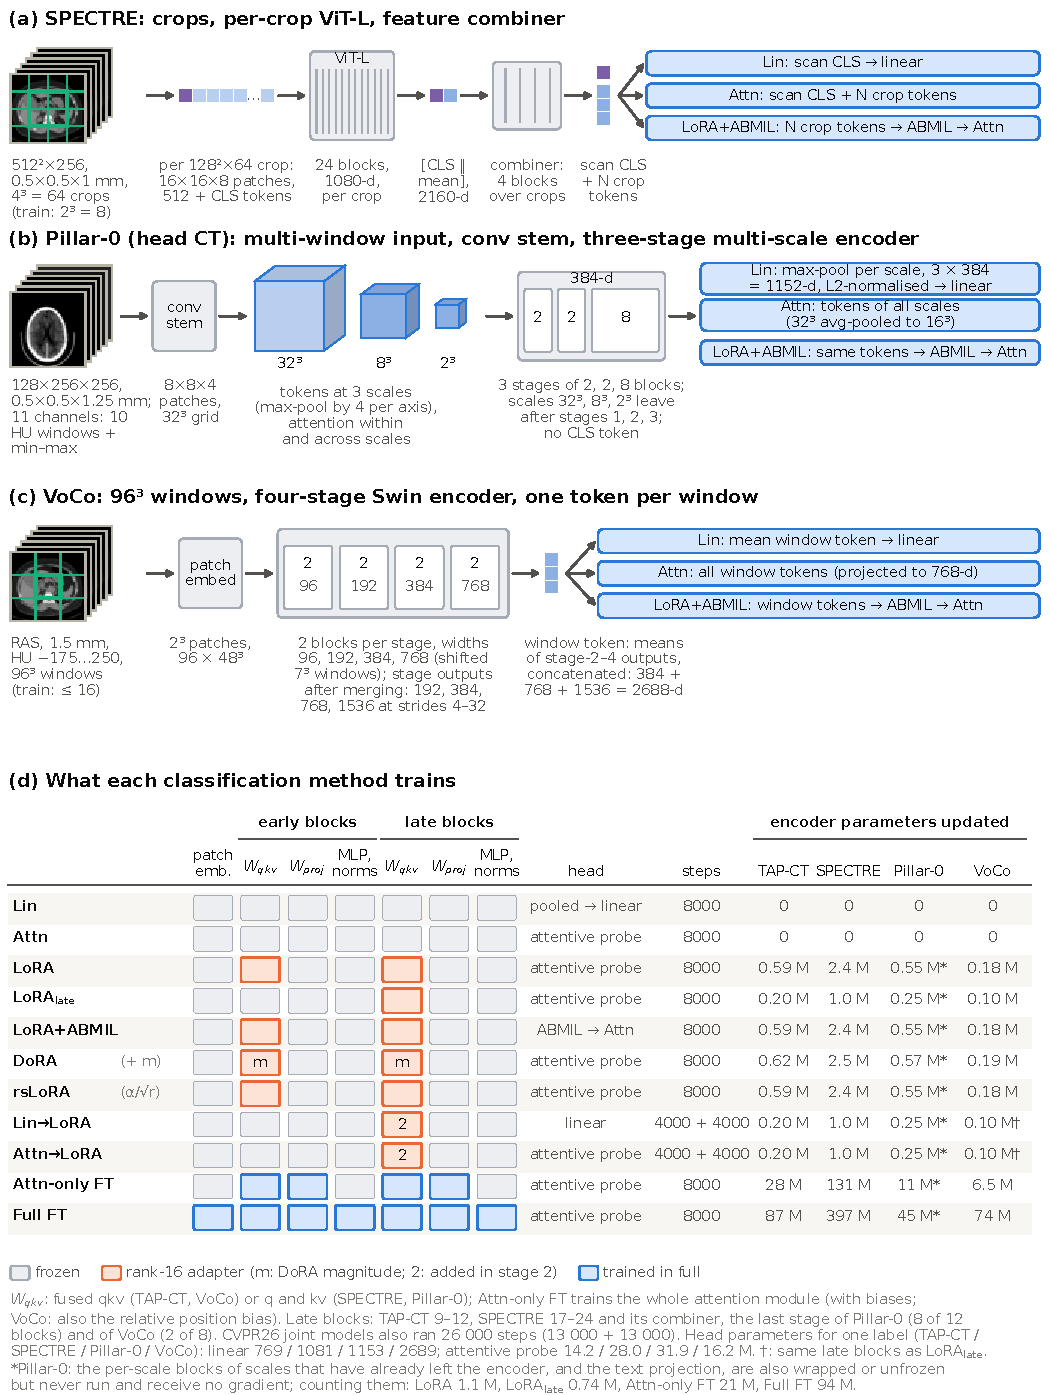
\includegraphics[width=0.88\textwidth,height=0.66\textheight,keepaspectratio]{figures/fig_arms.pdf}
\caption{Classification with SPECTRE, Pillar-0 and VoCo, drawn from the implementation (TAP-CT: Figure~\ref{fig:pipeline}). (a--c) How each backbone turns a volume into the tokens the heads read: SPECTRE encodes crops separately and summarizes them with its pretrained feature combiner; Pillar-0 encodes the whole head CT with a convolutional stem and a three-stage multi-scale transformer; VoCo encodes $96^3$ windows with a four-stage Swin encoder and forms one 2688-d token per window. (d) The encoder components each of the eleven methods trains, its head, its number of steps and the number of encoder parameters that receive a gradient; for Pillar-0 this excludes per-scale blocks that never run, and the note gives the logged counts that include them.}
\label{fig:arms}
\end{figure}

\begin{figure}[H]
\centering
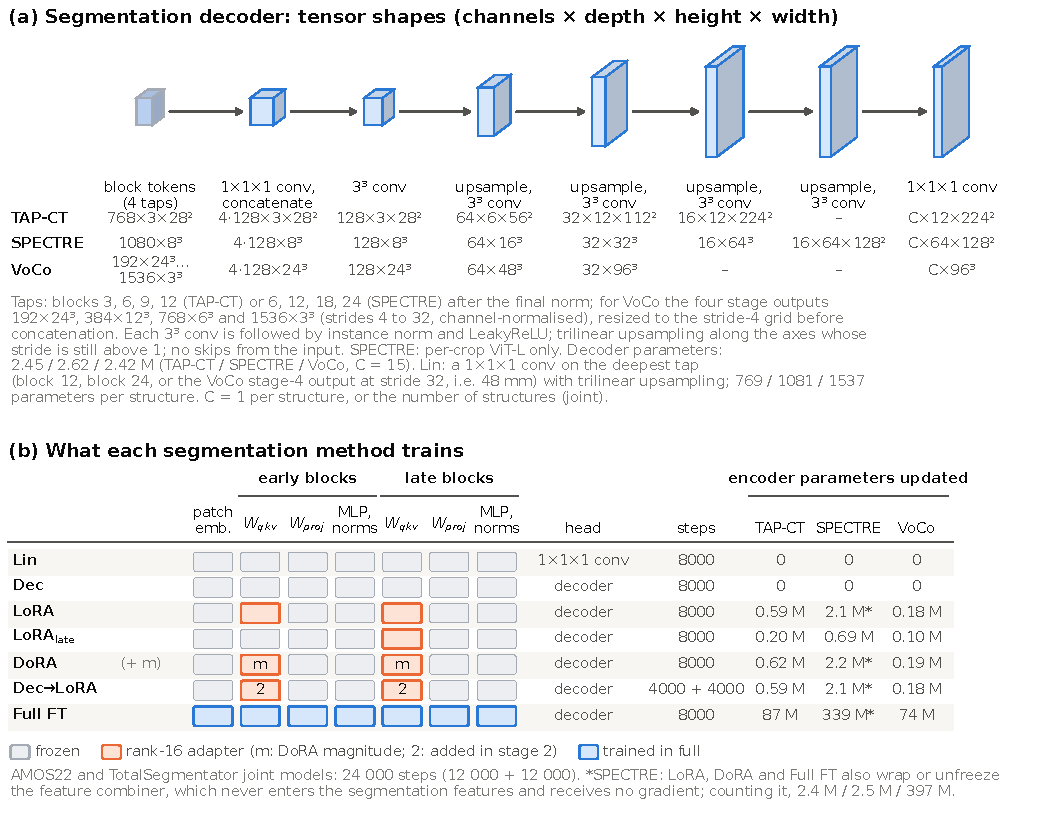
\includegraphics[width=\textwidth,height=0.74\textheight,keepaspectratio]{figures/fig_arms_seg.pdf}
\caption{Segmentation decoder and methods, drawn from the implementation. (a) Tensor shapes through the decoder for TAP-CT, SPECTRE and VoCo, from the four encoder taps to the $C$ output maps (one per structure). (b) The encoder components each of the seven methods trains and the number of encoder parameters that receive a gradient; the SPECTRE counts exclude the feature combiner, which the adapters wrap but which does not enter the segmentation features.}
\label{fig:armsseg}
\end{figure}

\paragraph{Input preprocessing.} Every volume is reoriented to the frame of the backbone's pretraining and resampled to its grid. TAP-CT: LPS, native slice spacing, in-plane trilinear resize to $224\times224$, depth padded with air to at least 12 slices and to a multiple of 4; HU clipped to $[-1008, 822]$ and standardised with the model's mean and standard deviation; windows of 12 slices with a stride of 3 slices plus a final window ending at the last slice (at most 32 windows per training step, all windows at evaluation). SPECTRE: RAS, $0.5\times0.5\times1$\,mm, centred $512\times512\times256$ field of view padded with the scan minimum, HU in $[-1000, 1000]$ scaled to $[0,1]$; a $4\times4\times4$ grid of 64 crops of $128\times128\times64$ voxels at evaluation and a random contiguous $2\times2\times2$ sub-grid of 8 crops at training; each crop is summarised by its CLS token concatenated with its mean patch token before the feature combiner. Pillar-0: LPI, $0.5\times0.5\times1.25$\,mm, centred $128\times256\times256$ volume, eleven input channels (ten fixed centre/width windows and a per-volume min--max channel), one forward pass; the linear head reads the model's L2-normalised pooled embedding (three scales concatenated, 1152-d), the attentive head reads the tokens of the three scales, any scale with more than 4096 tokens being average-pooled on its grid. VoCo: RAS, 1.5\,mm isotropic, HU in $[-175, 250]$ scaled to $[0,1]$, padded to at least $96^3$ and covered by non-overlapping $96^3$ windows (the last window shifted to the border; at most 16 windows per training step); each window becomes one 2688-dimensional token, the concatenation of the spatial means of the stage-2, 3 and 4 outputs, standardised per channel with running statistics (momentum 0.01) that are stored with the checkpoint. For segmentation, TAP-CT keeps the classification grid (in-plane 224, native depth) and crops of $12\times224\times224$ voxels; SPECTRE resamples to 1\,mm and uses crops of $64\times128\times128$ voxels; VoCo resamples to 1.5\,mm and uses $96^3$ crops. A training crop is centred on a random foreground voxel of the run's structures with probability 0.67 and placed uniformly otherwise; volumes smaller than the crop are padded with the image minimum. At evaluation the whole volume is covered by a sliding window with Gaussian weighting (overlap 0.5 for TAP-CT and VoCo, 0.25 for SPECTRE) and Dice is computed on the backbone's working grid, without post-processing.

\paragraph{Heads.} The linear head is dropout (0.2) followed by one linear layer on the pooled feature: the mean of the window CLS tokens for TAP-CT (768-d), the feature combiner's CLS token for SPECTRE (1080-d), the pooled image embedding for Pillar-0 (1152-d) and the mean window token for VoCo (2688-d). The attentive probe prepends a learnable CLS token to the token set (the window CLS tokens for TAP-CT, the combiner tokens for SPECTRE, the multi-scale tokens for Pillar-0, the window tokens for VoCo; VoCo's tokens are first projected from 2688 to 768 dimensions), applies two pre-norm transformer blocks with eight-head self-attention and a GELU feed-forward layer of ratio 4, normalises the CLS output and maps it through dropout (0.2) and a linear layer. LoRA+ABMIL pools the window or crop tokens by gated attention \citep{ilse2018abmil}, $a_i=\mathrm{softmax}_i\big(\bm{w}^\top(\tanh(\bm{V}\bm{x}_i)\odot\sigma(\bm{U}\bm{x}_i))\big)$ with hidden size 128, and feeds the pooled token to the attentive probe. The segmentation linear probe is a $1\times1\times1$ convolution on the deepest grid (TAP-CT block 12, SPECTRE block 24, VoCo stage 4 at stride 32), upsampled trilinearly. The decoder projects each of the four grids to 128 channels with a $1\times1\times1$ convolution, resizes them to a common grid (the token grid for the two ViTs, the stride-4 grid for VoCo), concatenates them (512 channels), fuses them with a $3^3$ convolution, instance normalisation and leaky ReLU to 128 channels, then applies stages of trilinear $\times2$ upsampling followed by the same convolution block that halves the channels (to a minimum of 16) until the voxel grid is reached (three stages for TAP-CT, four for SPECTRE, two for VoCo), and ends with a $1\times1\times1$ convolution to one logit per structure. It has 2.45\,M (TAP-CT), 2.62\,M (SPECTRE) and 2.42\,M (VoCo) parameters plus $17C$ or $33C$ for $C$ structures, and no skip connections from the input.

\paragraph{Adapters.} LoRA \citep{hu2022lora} replaces a frozen projection $\bm{W}_0\bm{x}$ by $\bm{W}_0\bm{x}+\tfrac{\alpha}{r}\bm{B}\bm{A}\,\mathrm{drop}(\bm{x})$ with $r=16$, $\alpha=32$ and dropout 0.1; $\bm{A}$ is initialised Kaiming-uniform and $\bm{B}$ at zero, so training starts from the pretrained model. It is applied to the fused query/key/value projection of every TAP-CT and VoCo block and to the separate query and key/value projections of every SPECTRE block, of SPECTRE's feature combiner, and of every Pillar-0 block. Late adapters cover TAP-CT blocks 9--12, SPECTRE blocks 17--24 and its feature combiner, the third stage of Pillar-0 (8 of 12 blocks) and the fourth stage of VoCo (2 of 8 blocks). rsLoRA scales the update by $\alpha/\sqrt{r}$ instead of $\alpha/r$. DoRA \citep{liu2024dora} rescales each row of the adapted weight to a learned magnitude $\bm{m}$, $\bm{W}=\bm{m}\odot(\bm{W}_0+\tfrac{\alpha}{r}\bm{B}\bm{A})/\lVert\bm{W}_0+\tfrac{\alpha}{r}\bm{B}\bm{A}\rVert_{\text{row}}$, with $\bm{m}$ initialised to the row norms of $\bm{W}_0$; the magnitude is a two-dimensional parameter and receives weight decay like the adapter matrices. Attention-only fine-tuning unfreezes every parameter of the attention modules that LoRA would adapt (query, key, value and output projections with their biases, and for VoCo the relative position bias). In segmentation the SPECTRE adapters and full fine-tuning also cover the feature combiner, which the segmentation path does not evaluate; those parameters receive no gradient.

\paragraph{Two-stage methods.} Lin$\to$LoRA and Attn$\to$LoRA take the probe weights (for VoCo also the running standardisation statistics of the window tokens) from the parent run's checkpoint at step 4000 of its 8000-step schedule, add late-block LoRA with $\bm{B}=0$, and train 4000 further steps with a fresh optimiser and schedule. Dec$\to$LoRA takes the decoder from the Dec run at the midpoint of its schedule (step 4000; step 12\,000 for the 24\,000-step joint models) and trains all-block LoRA with the decoder for the second half.

\paragraph{Optimisation.} AdamW uses $\beta=(0.9, 0.999)$ and $\epsilon=10^{-8}$ (the framework defaults; no run overrides them). The learning rate rises linearly from 1\% of its peak over the first 10\% of the steps and then follows a cosine to $10^{-6}$. Weight decay is applied to parameters of dimension two or more, excluding biases and normalisation weights. Gradients are not clipped. Classification trains at batch size 1 without gradient accumulation; segmentation at a micro-batch of 2 crops with accumulation 2, so four crops per step. The classification loss for a case with logits $\bm{z}$, labels $\bm{y}$ and known-label mask $\bm{m}$ is
\begin{equation}
\mathcal{L}_{\text{cls}}=\frac{1}{B}\sum_{b=1}^{B}\sum_{t} m_{bt}\,\mathrm{BCE}(z_{bt}, y_{bt}; w_t), \qquad w_t=\mathrm{clip}\Big(\frac{n^{-}_t}{n^{+}_t}, 0.05, 20\Big),
\label{eq:lcls}
\end{equation}
where $\mathrm{BCE}(\cdot;w_t)$ is the binary cross-entropy with positive weight $w_t$ computed from the negative and positive counts of label $t$ in the training split. The segmentation loss per case $b$ and structure $c$, with $\bm{p}=\sigma(\bm{z})$ over the $V$ voxels of a crop and reference $\bm{y}$, is
\begin{equation}
\mathcal{L}_{\text{seg}}=\frac{1}{BC}\sum_{b,c}\Big[1-\frac{2\sum_v p_{bcv}y_{bcv}+1}{\sum_v p_{bcv}+\sum_v y_{bcv}+1}+\frac{1}{V}\sum_v \mathrm{BCE}(z_{bcv},y_{bcv})\Big].
\label{eq:lseg}
\end{equation}
In the joint CVPR26 models the three sources are sampled in the ratio 10:8:8 (AMOS, COVID-CTset, LUNA25); every other run cycles one shuffled training set.


\begin{table}[H]
\centering
\caption{Classification settings per method. LoRA-type adapters have rank 16, $\alpha=32$ and dropout 0.1. Learning rate and weight decay apply to every trained parameter unless a backbone/head pair is given. All runs: AdamW, 8000 steps (two-stage: 4000 + 4000), batch size 1, warm-up 10\%, cosine to $10^{-6}$, bf16, head dropout 0.2.}
\label{tab:optim}
\adjustbox{max width=\textwidth,max totalheight=0.8\textheight}{\small
\begin{tabular}{@{}llll@{}}
\toprule
Method & Trained in the encoder & Head & Learning rate / weight decay \\
\midrule
Lin & nothing & linear & $10^{-3}$ / 0 \\
Attn & nothing & attentive & $10^{-4}$ / 0.01 \\
LoRA & LoRA on q, k, v of every block & attentive & $10^{-4}$ / 0.01 \\
LoRA$_{\text{late}}$ & LoRA on q, k, v of the late blocks & attentive & $10^{-4}$ / 0.01 \\
LoRA+ABMIL & as LoRA & ABMIL then attentive & $10^{-4}$ / 0.01 \\
DoRA & DoRA on q, k, v of every block & attentive & $10^{-4}$ / 0.01 \\
rsLoRA & LoRA, scale $\alpha/\sqrt{r}$ & attentive & $10^{-4}$ / 0.01 \\
Lin$\to$LoRA & late LoRA from step 4000 of Lin & linear (inherited) & $10^{-4}$ / 0.01 \\
Attn$\to$LoRA & late LoRA from step 4000 of Attn & attentive (inherited) & $10^{-4}$ / 0.01 \\
Attn-only FT & all attention parameters & attentive & encoder $2\times10^{-5}$ / 0.05, head $10^{-4}$ / 0.01 \\
Full FT & every parameter & attentive & encoder $2\times10^{-5}$ / 0.05, head $10^{-4}$ / 0.01 \\
\midrule
\multicolumn{4}{@{}l}{\textit{Repeats and controls (Appendix~\ref{app:revision})}} \\
Full FT, lower LR & every parameter & attentive & encoder $5\times10^{-6}$ / 0.05, head $10^{-4}$ / 0.01 \\
Full FT, layer decay & every parameter, LR $\times0.75$ per block from the top & attentive & encoder $2\times10^{-5}$ / 0.05, head $10^{-4}$ / 0.01 \\
Full FT, accumulation & every parameter; accumulation 8, clipping 1.0, 1000 steps & attentive & as Full FT \\
MLP-only FT & both MLP layers of every block & attentive & encoder $2\times10^{-5}$ / 0.05, head $10^{-4}$ / 0.01 \\
rsLoRA, matched LR & LoRA, scale $\alpha/\sqrt{r}$ & attentive & $2.5\times10^{-5}$ / 0.01 \\
\bottomrule
\end{tabular}}
\end{table}

\begin{table}[H]
\centering
\caption{Segmentation settings per method. All runs: AdamW, 8000 steps (24\,000 for the AMOS22 and TotalSegmentator joint models; two-stage methods split the budget in halves), four crops per step, warm-up 10\%, cosine to $10^{-6}$, bf16. LoRA-type adapters as in Table~\ref{tab:optim}.}
\label{tab:optimseg}
\adjustbox{max width=\textwidth,max totalheight=0.8\textheight}{\small
\begin{tabular}{@{}llll@{}}
\toprule
Method & Trained in the encoder & Head & Learning rate / weight decay \\
\midrule
Lin & nothing & linear probe & $10^{-2}$ / 0 \\
Dec & nothing & decoder & $10^{-3}$ / $10^{-4}$ \\
LoRA & LoRA on q, k, v of every block & decoder & $10^{-4}$ / $10^{-4}$ \\
LoRA$_{\text{late}}$ & LoRA on q, k, v of the late blocks & decoder & $10^{-4}$ / $10^{-4}$ \\
DoRA & DoRA on q, k, v of every block & decoder & $10^{-4}$ / $10^{-4}$ \\
Full FT & every parameter & decoder & encoder $2\times10^{-5}$, head $10^{-3}$ / $10^{-4}$ \\
Dec$\to$LoRA & all-block LoRA from the midpoint of Dec & decoder (inherited) & $10^{-4}$ / $10^{-4}$ \\
\midrule
\multicolumn{4}{@{}l}{\textit{Controls (Appendix~\ref{app:revision})}} \\
From scratch & every parameter, encoder re-initialised & decoder & as Full FT \\
Compute-matched per-structure & Dec, LoRA, Full FT at 1600 steps per structure & decoder & as above \\
\bottomrule
\end{tabular}}
\end{table}

\paragraph{Model selection and per-case outputs.} Every 1000 steps the selection and held-out splits are evaluated and a checkpoint of the trained parameters is written; the checkpoint with the highest selection macro AUROC (mean over labels with both classes present) or mean Dice (mean over structures of the mean over cases in which the structure is present in the reference or the prediction) is kept, ties keeping the earlier checkpoint. For TotalSegmentator only the selection split is evaluated during training; the held-out split is evaluated afterwards with the selected checkpoint, and the recomputed selection Dice is required to match the recorded value within 0.005. Per case, the held-out probability of every known label (classification) and the Dice of every structure (segmentation) at the selected checkpoint are stored and are the input of every number in this paper. Dice thresholds the logits at 0; a structure enters a case's mean when the reference or the prediction contains it, so a false-positive structure scores 0 and an absent, unpredicted structure is skipped.

\clearpage
\section{Statistical procedure}
\label{app:stats}
Every number in this paper is computed by one script from the stored per-case predictions of the selected checkpoint of every run (\numRunsMainN{} main runs and \numRunsRevisionN{} repeats and controls; the classification files hold the held-out probability of every known label of every case, the segmentation files the Dice of every structure of every case).

\paragraph{Per-run metrics.} AUROC is the Mann--Whitney statistic with midranks (tied scores count one half); a label is skipped for a run when its selection or held-out split has fewer than two cases or a single class, which did not occur. Dice per structure is the mean over the held-out cases in which the structure is present in the reference or the prediction; an absent, unpredicted structure is skipped and a false-positive structure counts as 0. Cohort and dataset means (Tables~\ref{tab:cls} and~\ref{tab:seg}) are means over the labels or structures of complete cells. The recomputed selection-split macro metric was compared with the value logged during training for every run: all \numSelcheckClsRunsN{} classification runs agree to $10^{-7}$, and all but one of the \numSelcheckSegRunsN{} segmentation runs within $2\times10^{-3}$ (\numSegrecompRunsN{} segmentation runs had their per-case Dice re-inferred from the selected checkpoint after training; the one exception differs by $2.01\times10^{-3}$).

\paragraph{Did-not-train rule.} For each backbone and method, the median over label--mode pairs of the standard deviation of the held-out probabilities is computed; a median below \numSpreadMinValue{} flags a method that did not train. Only SPECTRE Full FT is flagged (\numSpreadSpectreFullft{}; every other method on TAP-CT, SPECTRE and Pillar-0 is at least \numSpreadOthermin{}). It stays in the per-cohort tables, the paired tests and the Full FT $-$ Lin estimate, and leaves the ranks and every average over methods. VoCo spreads are reported (Table~\ref{tab:spread}) but the rule is not applied to VoCo, whose methods have small spreads at held-out AUROCs well above chance.

\paragraph{Paired tests.} Per backbone, cohort, mode (per-task, joint) and label, every method is compared with the baselines Lin, LoRA, Attn and Full FT (classification; two-sided DeLong test of the AUROC difference on the same cases \citep{delong1988}) or Lin, Dec and LoRA (segmentation; paired case bootstrap of the mean Dice difference, 4000 resamples shared by every comparison of the same group, two-sided bootstrap $p$). Pairs require identical case sets; none had to be skipped. $p$-values are Benjamini--Hochberg adjusted \citep{benjamini1995fdr} within each family of comparisons (task, baseline, VoCo or not), and ``significant'' means an adjusted $p$ below 0.05; \numDelongTestsN{} DeLong tests and \numSegpairedTestsN{} bootstrap tests were made.

\paragraph{Label-level estimates.} The unit is one label (structure) on one backbone. For a comparison A $-$ B its value is the mean over the per-task and joint modes of the difference of the two methods' held-out metric (both modes must exist); for joint minus per-task it is the mean over the methods trained in both modes. The reported mean is over the labels of a backbone, or pooled over TAP-CT, SPECTRE and Pillar-0 (\numCiClsloralinAllLabelsN{} label--backbone units in classification, \numCiSegdeclinAllLabelsN{} in segmentation). Its 95\% interval is a percentile bootstrap with 4000 resamples that draws cohort--backbone clusters with replacement, then labels within each drawn cluster, and then replaces each drawn label's value by one of 1000 case-level resamples of that label (positives and negatives resampled separately in classification, with the same case indices for every term of the difference; all cases in segmentation). Besides the comparisons with the linear probe (Lin) and the frozen decoder (Dec), every method with the attentive head is compared with the frozen attentive probe (matched head), and LoRA $-$ Lin is also computed without FDG-PET/CT and the COVID-CTset label. Table~\ref{tab:cis} also gives the interval without the case stage. The number of cohort--backbone clusters with a positive mean is reported next to every estimate.

\paragraph{Ranks.} A slot is a label (structure) on one backbone in one mode with every method of the task present (minus methods that did not train); methods are ranked by held-out AUROC or Dice with ties sharing the average rank. Classification has \numRankSlotsN{} slots over the three main backbones and \numVocorankSlotsN{} on VoCo; segmentation \numSegrankSlotsN{} and \numVocosegrankSlotsN{} (TotalSegmentator per-structure slots lack three methods and are not ranked). Figure~\ref{fig:overview} pools all \numRankallSlotsN{} and \numSegrankallSlotsN{} slots; each slot is ranked within its backbone.

\paragraph{Seeds, controls and convergence.} Seed repeats are compared through cohort means per seed and the number of cohort--seed pairs in which one method is ahead of another; full fine-tuning variants through the selection-split AUROC, the number of cohorts whose run trained (median spread at least \numSpreadMinValue{}) and, for the variant with the highest selection AUROC, its label-level difference to Lin and LoRA; compute-matched models through the mean over structures of joint minus matched Dice. Convergence is the share of runs whose selected checkpoint is the last or one of the last two validations. All random draws use fixed seeds, so the script is deterministic.


\clearpage
\section{Paired comparisons and further analyses}
\label{app:paired}

\begin{figure}[H]
\centering
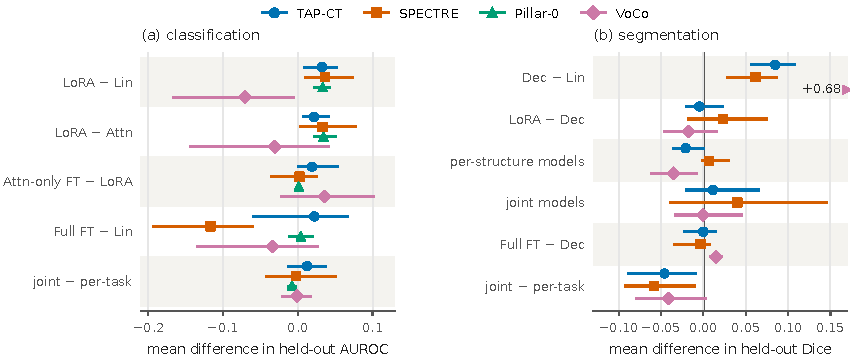
\includegraphics[width=\textwidth,height=0.74\textheight,keepaspectratio]{figures/fig_key.pdf}
\caption{Label-level mean difference in held-out AUROC (a) or Dice (b) for the comparisons of Table~\ref{tab:key}, per backbone, with the 95\% interval over cohorts, labels and held-out cases; 0 means no difference. VoCo was run on three classification cohorts. A triangle at the axis edge marks an estimate beyond the axis, with its value printed. The SPECTRE Full FT $-$ Lin estimate includes runs that did not train.}
\label{fig:key}
\end{figure}

\begin{table}[H]
\centering
\caption{Classification headline: pooled held-out AUROC per backbone (mean over all label comparisons, $n$ = labels $\times$ \{per-task, joint\}), and per-label paired comparisons of LoRA against the linear probe and against full fine-tuning (DeLong, Benjamini--Hochberg; ``sig.'' = corrected $p<0.05$ in the stated direction). The mean gain of LoRA over the probe is similar for small and large held-out splits ($\numSigbysizeSmallMeandiff$ below 100 cases, $\numSigbysizeLargeMeandiff$ above 400) but significant in \numSigbysizeSmallSig\% and \numSigbysizeLargeSig\% of these comparisons; every comparison above 400 cases is from the hemorrhage cohort.}
\label{tab:headline}
\adjustbox{max width=\textwidth,max totalheight=0.8\textheight}{\footnotesize\begin{tabular}{lrccccrrrrrr}
\toprule
 & & \multicolumn{4}{c}{Pooled AUROC} & \multicolumn{3}{c}{LoRA vs.\ linear probe} & \multicolumn{3}{c}{LoRA vs.\ full fine-tuning} \\
\cmidrule(lr){3-6}\cmidrule(lr){7-9}\cmidrule(lr){10-12}
Backbone & $n$ & Lin & LoRA & Attn-only FT & Full FT & Mean $\Delta$ & LoRA better (\%) & sig.\ (\%) & Mean $\Delta$ & LoRA better (\%) & FT sig.\ better (\%) \\
\midrule
TAP-CT & 78 & 0.727 & 0.760 & 0.779 & 0.749 & +0.032 & 78 & 17 & +0.010 & 55 & 6 \\
SPECTRE & 66 & 0.718 & 0.755 & 0.757 & 0.601 & +0.037 & 74 & 9 & +0.153 & 94 & 2 \\
Pillar-0 & 12 & 0.887 & 0.920 & 0.922 & 0.891 & +0.033 & 92 & 83 & +0.029 & 100 & 0 \\
\bottomrule
\end{tabular}
}
\end{table}

\begin{table}[H]
\centering
\caption{Classification methods: trainable parameters of a single-label model as logged (head included; for Pillar-0 the count includes parameters of per-scale blocks that never run and receive no gradient, so the encoder parameters updated are about half, Figure~\ref{fig:arms}); mean rank within each of the \numRankSlotsN{} label--mode pairs ($\downarrow$; on SPECTRE among the ten methods that trained); share of pairs within 0.01 AUROC of the best method ($\uparrow$); mean AUROC deficit to the best method ($\downarrow$). \textbf{Bold}: best, \underline{underlined}: second best of each rank and score column. Full FT's pooled values exclude SPECTRE, where it did not train, so they are not comparable with the other methods' and are not marked. Choosing the method per label on the selection split finds the held-out best in \numSelectHit\% of pairs and lowers the mean deficit from $\numRegretAttnft$ (always attention-only fine-tuning) to $\numSelectRegret$, at eleven runs per label instead of one.}
\label{tab:methods}
\adjustbox{max width=\textwidth,max totalheight=0.8\textheight}{\footnotesize\begin{tabular}{lrrrccccrr}
\toprule
 & \multicolumn{3}{c}{Trainable parameters} & \multicolumn{4}{c}{Mean rank (1 = best)} & Within 0.01 & $\Delta$ to best \\
\cmidrule(lr){2-4}\cmidrule(lr){5-8}
Method & TAP-CT & SPECTRE & Pillar-0 & TAP-CT & SPECTRE & Pillar-0 & All & of best (\%) & (AUROC) \\
\midrule
Lin & 769 & 1081 & 1153 & 7.62 & 7.15 & 9.33 & 7.55 & 7 & 0.081 \\
Attn & 14.2\,M & 28.0\,M & 31.9\,M & 6.71 & 6.96 & 9.75 & 7.05 & 10 & 0.074 \\
LoRA & 14.8\,M & 30.4\,M & 33.0\,M & \underline{4.76} & 4.94 & 3.83 & \underline{4.76} & 23 & 0.046 \\
LoRA$_{\text{late}}$ & 14.4\,M & 29.1\,M & 32.6\,M & 5.46 & 5.50 & 7.17 & 5.61 & 17 & 0.054 \\
LoRA+ABMIL & 15.0\,M & 30.7\,M & 33.3\,M & 5.61 & \textbf{4.02} & 4.33 & 4.84 & \underline{26} & \underline{0.045} \\
DoRA & 14.8\,M & 30.5\,M & 33.0\,M & 5.50 & 4.72 & 3.67 & 5.03 & 19 & 0.049 \\
rsLoRA & 14.8\,M & 30.4\,M & 33.0\,M & 7.17 & 5.31 & \textbf{2.67} & 6.04 & 18 & 0.065 \\
Lin$\to$LoRA & 0.20\,M & 1.0\,M & 0.74\,M & 7.48 & 5.27 & 6.58 & 6.47 & 11 & 0.064 \\
Attn$\to$LoRA & 14.4\,M & 29.1\,M & 32.6\,M & 6.90 & 6.47 & 7.67 & 6.78 & 13 & 0.069 \\
Attn-only FT & 42.5\,M & 159\,M & 53.2\,M & \textbf{3.38} & \underline{4.67} & \underline{3.25} & \textbf{3.91} & \textbf{38} & \textbf{0.036} \\
Full FT & 101\,M & 425\,M & 126\,M & 5.44 & -- & 7.75 & 5.74 & 31 & 0.055 \\
\bottomrule
\end{tabular}
}
\end{table}

\begin{table}[H]
\centering
\caption{Label-level differences with 95\% intervals. Each label (or structure) counts once, with its per-task and joint differences averaged (except the two LoRA $-$ Dec sub-rows). Intervals are percentile bootstraps (4000 resamples) over cohort--backbone groups and labels within them, without and with a third stage that resamples the held-out cases of each drawn label (Appendix~\ref{app:stats}). Pillar-0 has one cohort, so its interval resamples labels and cases only. The last column counts the cohorts (datasets) with a positive mean difference.}
\label{tab:cis}
\adjustbox{max width=\textwidth,max totalheight=0.8\textheight}{\footnotesize\begin{tabular}{llrrccc}
\toprule
 & & & & \multicolumn{2}{c}{95\% interval, resampling} & \\
\cmidrule(lr){5-6}
Comparison & Backbone & $n$ & Mean & cohorts, labels & + cases & Cohorts $>0$ \\
\midrule
LoRA $-$ Lin & all & 78 & +0.034 & [+0.019, +0.049] & [+0.017, +0.052] & 9/10 \\
LoRA $-$ Lin & TAP-CT & 39 & +0.032 & [+0.009, +0.049] & [+0.007, +0.053] & 4/5 \\
LoRA $-$ Lin & SPECTRE & 33 & +0.037 & [+0.013, +0.068] & [+0.009, +0.075] & 4/4 \\
LoRA $-$ Lin & Pillar-0 & 6 & +0.033 & [+0.021, +0.042] & [+0.021, +0.044] & 1/1 \\
LoRA $-$ Lin & VoCo & 16 & -0.071 & [-0.162, -0.011] & [-0.168, -0.005] & 0/3 \\
\addlinespace[2pt]
LoRA $-$ Attn & all & 78 & +0.027 & [+0.013, +0.047] & [+0.012, +0.048] & 10/10 \\
LoRA $-$ Attn & TAP-CT & 39 & +0.022 & [+0.009, +0.039] & [+0.006, +0.042] & 5/5 \\
LoRA $-$ Attn & SPECTRE & 33 & +0.033 & [+0.007, +0.074] & [+0.003, +0.078] & 4/4 \\
LoRA $-$ Attn & Pillar-0 & 6 & +0.034 & [+0.021, +0.051] & [+0.021, +0.052] & 1/1 \\
LoRA $-$ Attn & VoCo & 16 & -0.031 & [-0.150, +0.033] & [-0.145, +0.043] & 1/3 \\
\addlinespace[2pt]
Attn-only FT $-$ LoRA & all & 78 & +0.011 & [-0.005, +0.026] & [-0.007, +0.029] & 7/10 \\
Attn-only FT $-$ LoRA & TAP-CT & 39 & +0.019 & [+0.002, +0.053] & [-0.001, +0.054] & 4/5 \\
Attn-only FT $-$ LoRA & SPECTRE & 33 & +0.002 & [-0.037, +0.023] & [-0.037, +0.026] & 2/4 \\
Attn-only FT $-$ LoRA & Pillar-0 & 6 & +0.001 & [0.000, +0.003] & [-0.002, +0.004] & 1/1 \\
Attn-only FT $-$ LoRA & VoCo & 16 & +0.036 & [-0.020, +0.097] & [-0.024, +0.102] & 2/3 \\
\addlinespace[2pt]
Full FT $-$ Lin & all & 78 & -0.038 & [-0.101, +0.017] & [-0.103, +0.019] & 5/10 \\
Full FT $-$ Lin & TAP-CT & 39 & +0.022 & [-0.057, +0.064] & [-0.061, +0.068] & 4/5 \\
Full FT $-$ Lin & SPECTRE & 33 & -0.117 & [-0.195, -0.063] & [-0.195, -0.059] & 0/4 \\
Full FT $-$ Lin & Pillar-0 & 6 & +0.004 & [-0.011, +0.019] & [-0.013, +0.021] & 1/1 \\
Full FT $-$ Lin & VoCo & 16 & -0.034 & [-0.133, +0.018] & [-0.136, +0.027] & 1/3 \\
\addlinespace[2pt]
Joint $-$ per-task & all & 78 & +0.004 & [-0.017, +0.027] & [-0.021, +0.030] & 6/10 \\
Joint $-$ per-task & TAP-CT & 39 & +0.012 & [-0.005, +0.032] & [-0.014, +0.038] & 3/5 \\
Joint $-$ per-task & SPECTRE & 33 & -0.003 & [-0.035, +0.049] & [-0.044, +0.051] & 3/4 \\
Joint $-$ per-task & Pillar-0 & 6 & -0.008 & [-0.012, -0.003] & [-0.013, -0.001] & 0/1 \\
Joint $-$ per-task & VoCo & 16 & -0.001 & [-0.017, +0.012] & [-0.022, +0.018] & 2/3 \\
\addlinespace[2pt]
Dec $-$ Lin & all & 74 & +0.073 & [+0.049, +0.093] & [+0.049, +0.092] & 10/10 \\
Dec $-$ Lin & TAP-CT & 37 & +0.085 & [+0.055, +0.109] & [+0.055, +0.109] & 5/5 \\
Dec $-$ Lin & SPECTRE & 37 & +0.061 & [+0.028, +0.089] & [+0.027, +0.088] & 5/5 \\
Dec $-$ Lin & VoCo & 37 & +0.680 & [+0.430, +0.747] & [+0.433, +0.746] & 5/5 \\
\addlinespace[2pt]
LoRA $-$ Dec & all & 74 & +0.009 & [-0.014, +0.046] & [-0.015, +0.046] & 8/10 \\
LoRA $-$ Dec & TAP-CT & 37 & -0.005 & [-0.021, +0.023] & [-0.021, +0.024] & 4/5 \\
LoRA $-$ Dec & SPECTRE & 37 & +0.023 & [-0.017, +0.079] & [-0.018, +0.076] & 4/5 \\
LoRA $-$ Dec & VoCo & 37 & -0.018 & [-0.045, +0.017] & [-0.047, +0.016] & 2/5 \\
\addlinespace[2pt]
\quad per-structure models & all & 74 & -0.007 & [-0.021, +0.009] & [-0.022, +0.009] & 7/10 \\
\quad per-structure models & TAP-CT & 37 & -0.021 & [-0.035, +0.002] & [-0.036, +0.002] & 2/5 \\
\quad per-structure models & SPECTRE & 37 & +0.006 & [-0.001, +0.028] & [-0.003, +0.031] & 5/5 \\
\quad per-structure models & VoCo & 37 & -0.035 & [-0.062, -0.008] & [-0.062, -0.007] & 0/5 \\
\addlinespace[2pt]
\quad joint models & all & 74 & +0.026 & [-0.020, +0.092] & [-0.021, +0.093] & 8/10 \\
\quad joint models & TAP-CT & 37 & +0.011 & [-0.019, +0.067] & [-0.021, +0.066] & 4/5 \\
\quad joint models & SPECTRE & 37 & +0.040 & [-0.038, +0.148] & [-0.039, +0.147] & 4/5 \\
\quad joint models & VoCo & 37 & 0.000 & [-0.034, +0.047] & [-0.034, +0.047] & 2/5 \\
\addlinespace[2pt]
Full FT $-$ Dec & all & 74 & -0.002 & [-0.017, +0.009] & [-0.018, +0.009] & 6/10 \\
Full FT $-$ Dec & TAP-CT & 37 & 0.000 & [-0.025, +0.015] & [-0.024, +0.016] & 4/5 \\
Full FT $-$ Dec & SPECTRE & 37 & -0.003 & [-0.033, +0.008] & [-0.035, +0.009] & 2/5 \\
Full FT $-$ Dec & VoCo & 37 & +0.015 & [+0.008, +0.023] & [+0.007, +0.023] & 4/5 \\
\addlinespace[2pt]
Joint $-$ per-task & all & 74 & -0.052 & [-0.082, -0.021] & [-0.082, -0.022] & 0/10 \\
Joint $-$ per-task & TAP-CT & 37 & -0.046 & [-0.088, -0.009] & [-0.090, -0.008] & 0/5 \\
Joint $-$ per-task & SPECTRE & 37 & -0.058 & [-0.092, -0.010] & [-0.093, -0.009] & 0/5 \\
Joint $-$ per-task & VoCo & 37 & -0.041 & [-0.081, +0.002] & [-0.081, +0.004] & 2/5 \\
\bottomrule
\end{tabular}
}
\end{table}

\begin{table}[H]
\centering
\caption{Per-label paired comparisons of held-out AUROC against the linear probe and against full fine-tuning, over the per-task and joint modes (DeLong test; Benjamini--Hochberg correction within each baseline over the comparisons of TAP-CT, SPECTRE and Pillar-0). ``Better'' is the share of label--mode pairs in which the method's AUROC exceeds the baseline's; ``Sig.'' the share in which, in addition, the corrected $p<0.05$. SPECTRE Full FT did not train.}
\label{tab:paired}
\adjustbox{max width=\textwidth,max totalheight=0.8\textheight}{\footnotesize\begin{tabular}{lllrrrrr}
\toprule
Backbone & Baseline & Method & Labels & Mean $\Delta$AUROC & Better (\%) & Sig.\ better (\%) & Sig.\ worse (\%) \\
\midrule
TAP-CT & vs Lin & Attn & 78 & +0.011 & 59 & 4 & 0 \\
 &  & LoRA & 78 & +0.032 & 78 & 17 & 0 \\
 &  & LoRA$_{\text{late}}$ & 78 & +0.023 & 69 & 14 & 1 \\
 &  & LoRA+ABMIL & 78 & +0.024 & 68 & 12 & 1 \\
 &  & DoRA & 78 & +0.028 & 68 & 17 & 0 \\
 &  & rsLoRA & 78 & +0.003 & 55 & 5 & 5 \\
 &  & Lin$\to$LoRA & 78 & +0.001 & 51 & 5 & 1 \\
 &  & Attn$\to$LoRA & 78 & +0.008 & 56 & 9 & 0 \\
 &  & Attn-only FT & 78 & +0.051 & 83 & 24 & 0 \\
 &  & Full FT & 78 & +0.022 & 72 & 13 & 8 \\
\addlinespace[2pt]
TAP-CT & vs Full FT & Lin & 78 & -0.022 & 28 & 12 & 17 \\
 &  & Attn & 78 & -0.011 & 40 & 10 & 18 \\
 &  & LoRA & 78 & +0.010 & 55 & 18 & 6 \\
 &  & LoRA$_{\text{late}}$ & 78 & +0.001 & 44 & 18 & 6 \\
 &  & LoRA+ABMIL & 78 & +0.002 & 45 & 17 & 12 \\
 &  & DoRA & 78 & +0.006 & 51 & 17 & 9 \\
 &  & rsLoRA & 78 & -0.019 & 47 & 13 & 22 \\
 &  & Lin$\to$LoRA & 78 & -0.021 & 31 & 9 & 18 \\
 &  & Attn$\to$LoRA & 78 & -0.014 & 38 & 13 & 15 \\
 &  & Attn-only FT & 78 & +0.029 & 63 & 23 & 5 \\
\addlinespace[2pt]
SPECTRE & vs Lin & Attn & 66 & +0.004 & 50 & 3 & 2 \\
 &  & LoRA & 66 & +0.037 & 74 & 9 & 0 \\
 &  & LoRA$_{\text{late}}$ & 66 & +0.034 & 65 & 5 & 0 \\
 &  & LoRA+ABMIL & 66 & +0.052 & 77 & 12 & 2 \\
 &  & DoRA & 66 & +0.037 & 77 & 8 & 0 \\
 &  & rsLoRA & 66 & +0.028 & 70 & 9 & 0 \\
 &  & Lin$\to$LoRA & 66 & +0.035 & 71 & 6 & 0 \\
 &  & Attn$\to$LoRA & 66 & +0.016 & 59 & 6 & 2 \\
 &  & Attn-only FT & 66 & +0.039 & 70 & 3 & 3 \\
 &  & Full FT & 66 & -0.117 & 21 & 0 & 32 \\
\addlinespace[2pt]
SPECTRE & vs Full FT & Lin & 66 & +0.117 & 79 & 33 & 0 \\
 &  & Attn & 66 & +0.121 & 86 & 35 & 0 \\
 &  & LoRA & 66 & +0.153 & 94 & 44 & 2 \\
 &  & LoRA$_{\text{late}}$ & 66 & +0.151 & 95 & 44 & 0 \\
 &  & LoRA+ABMIL & 66 & +0.168 & 94 & 52 & 0 \\
 &  & DoRA & 66 & +0.154 & 92 & 44 & 2 \\
 &  & rsLoRA & 66 & +0.145 & 89 & 39 & 0 \\
 &  & Lin$\to$LoRA & 66 & +0.152 & 94 & 41 & 0 \\
 &  & Attn$\to$LoRA & 66 & +0.133 & 88 & 44 & 0 \\
 &  & Attn-only FT & 66 & +0.156 & 89 & 48 & 0 \\
\addlinespace[2pt]
Pillar-0 & vs Lin & Attn & 12 & -0.001 & 42 & 33 & 8 \\
 &  & LoRA & 12 & +0.033 & 92 & 83 & 0 \\
 &  & LoRA$_{\text{late}}$ & 12 & +0.016 & 75 & 67 & 0 \\
 &  & LoRA+ABMIL & 12 & +0.026 & 83 & 75 & 8 \\
 &  & DoRA & 12 & +0.034 & 92 & 83 & 0 \\
 &  & rsLoRA & 12 & +0.032 & 100 & 83 & 0 \\
 &  & Lin$\to$LoRA & 12 & +0.022 & 100 & 83 & 0 \\
 &  & Attn$\to$LoRA & 12 & +0.013 & 92 & 58 & 0 \\
 &  & Attn-only FT & 12 & +0.034 & 92 & 83 & 0 \\
 &  & Full FT & 12 & +0.004 & 67 & 50 & 17 \\
\addlinespace[2pt]
Pillar-0 & vs Full FT & Lin & 12 & -0.004 & 33 & 17 & 50 \\
 &  & Attn & 12 & -0.005 & 33 & 17 & 58 \\
 &  & LoRA & 12 & +0.029 & 100 & 67 & 0 \\
 &  & LoRA$_{\text{late}}$ & 12 & +0.012 & 58 & 33 & 25 \\
 &  & LoRA+ABMIL & 12 & +0.022 & 58 & 58 & 8 \\
 &  & DoRA & 12 & +0.030 & 83 & 67 & 0 \\
 &  & rsLoRA & 12 & +0.028 & 92 & 67 & 0 \\
 &  & Lin$\to$LoRA & 12 & +0.018 & 67 & 42 & 25 \\
 &  & Attn$\to$LoRA & 12 & +0.009 & 50 & 33 & 25 \\
 &  & Attn-only FT & 12 & +0.030 & 100 & 83 & 0 \\
\addlinespace[2pt]
\bottomrule
\end{tabular}
}
\end{table}

\begin{table}[H]
\centering
\caption{Per-structure paired comparisons of held-out Dice over the per-structure and joint modes against the linear probe and the frozen decoder (paired bootstrap of the mean per-case difference, 4000 resamples; Benjamini--Hochberg correction within each baseline). Pairing keeps the cases on which a structure enters the Dice of both methods (present in the reference or in either prediction), so the mean differences here can differ from the differences of structure means in Table~\ref{tab:seg}.}
\label{tab:segpaired}
\adjustbox{max width=\textwidth,max totalheight=0.8\textheight}{\footnotesize\begin{tabular}{lllrrrrr}
\toprule
Backbone & Baseline & Method & Pairs & Mean $\Delta$Dice & Better (\%) & Sig.\ better (\%) & Sig.\ worse (\%) \\
\midrule
TAP-CT & vs Lin & Dec & 74 & +0.086 & 96 & 93 & 4 \\
 &  & LoRA & 74 & +0.088 & 96 & 93 & 3 \\
 &  & LoRA$_{\text{late}}$ & 59 & +0.077 & 95 & 92 & 5 \\
 &  & DoRA & 59 & +0.078 & 95 & 90 & 5 \\
 &  & Full FT & 74 & +0.085 & 93 & 93 & 7 \\
 &  & Dec$\to$LoRA & 59 & +0.066 & 92 & 88 & 8 \\
\addlinespace[2pt]
TAP-CT & vs Dec & Lin & 74 & -0.086 & 4 & 4 & 93 \\
 &  & LoRA & 74 & +0.002 & 54 & 31 & 30 \\
 &  & LoRA$_{\text{late}}$ & 59 & -0.006 & 53 & 29 & 32 \\
 &  & DoRA & 59 & -0.006 & 53 & 25 & 25 \\
 &  & Full FT & 74 & -0.001 & 76 & 53 & 8 \\
 &  & Dec$\to$LoRA & 59 & -0.017 & 29 & 7 & 44 \\
\addlinespace[2pt]
SPECTRE & vs Lin & Dec & 74 & +0.061 & 92 & 86 & 5 \\
 &  & LoRA & 74 & +0.095 & 93 & 93 & 4 \\
 &  & LoRA$_{\text{late}}$ & 59 & +0.079 & 92 & 90 & 5 \\
 &  & DoRA & 59 & +0.088 & 93 & 90 & 7 \\
 &  & Full FT & 74 & +0.059 & 89 & 81 & 8 \\
 &  & Dec$\to$LoRA & 59 & +0.051 & 90 & 85 & 7 \\
\addlinespace[2pt]
SPECTRE & vs Dec & Lin & 74 & -0.061 & 8 & 5 & 86 \\
 &  & LoRA & 74 & +0.034 & 80 & 57 & 8 \\
 &  & LoRA$_{\text{late}}$ & 59 & +0.032 & 69 & 46 & 8 \\
 &  & DoRA & 59 & +0.041 & 76 & 54 & 12 \\
 &  & Full FT & 74 & -0.002 & 54 & 38 & 20 \\
 &  & Dec$\to$LoRA & 59 & +0.004 & 69 & 20 & 12 \\
\addlinespace[2pt]
\bottomrule
\end{tabular}
}
\end{table}

\begin{figure}[H]
\centering
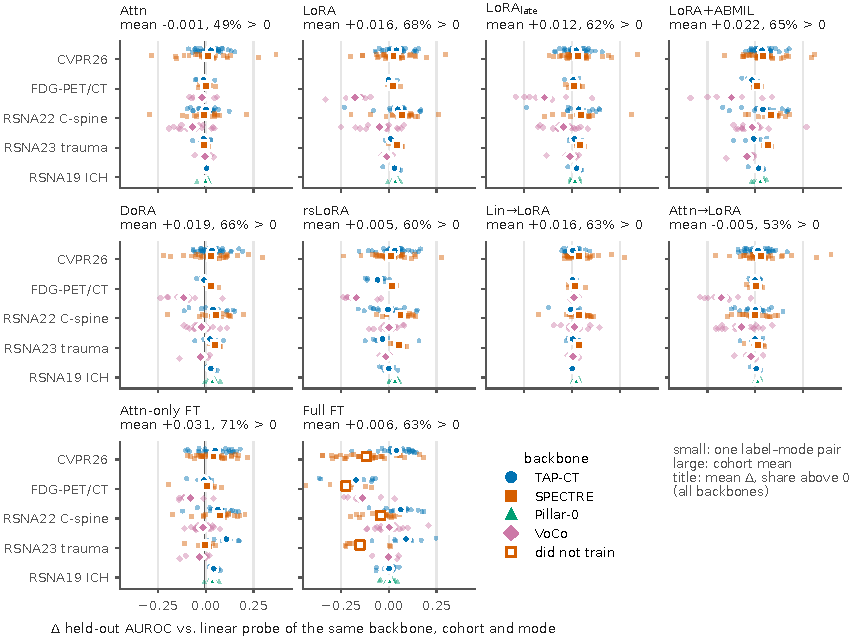
\includegraphics[width=\textwidth,height=0.74\textheight,keepaspectratio]{figures/fig_methods.pdf}
\caption{Per-label change in held-out AUROC of each classification method relative to the linear probe of the same backbone, cohort and mode, one panel per method; rows are cohorts, color is the backbone, small markers are single label--mode comparisons and large markers the mean per cohort and backbone. Titles give the mean change and the share above zero over the pairs of all four backbones that trained. SPECTRE Full FT did not train; its cohort means are drawn open and left out of the title.}
\label{fig:methods}
\end{figure}

\begin{figure}[H]
\centering
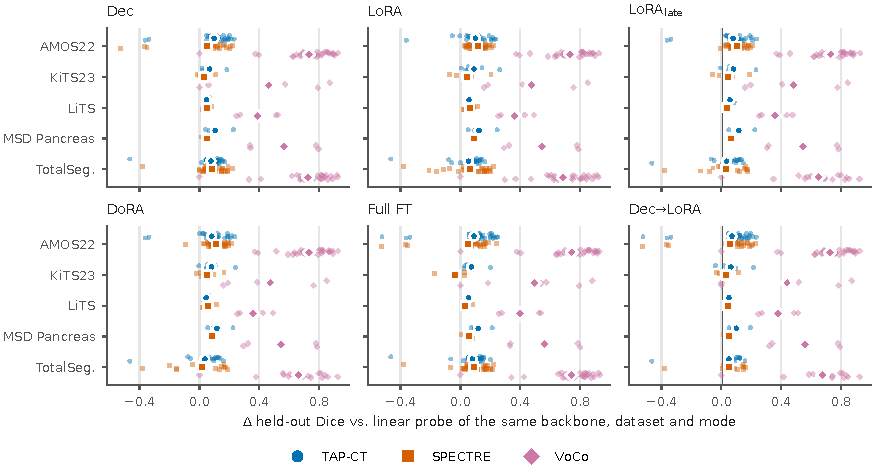
\includegraphics[width=\textwidth,height=0.74\textheight,keepaspectratio]{figures/fig_seg_methods.pdf}
\caption{Per-structure change in held-out Dice of each segmentation method relative to the linear probe of the same backbone, dataset and mode, one panel per method; rows are datasets, color is the backbone, small markers are single structure--mode comparisons and large markers the mean per dataset and backbone. VoCo's linear probe reads one token per 48\,mm and segments almost nothing, so its changes are far larger than those of the two ViTs.}
\label{fig:segmethods}
\end{figure}

\begin{table}[H]
\centering
\caption{Encoder adaptation on top of the frozen decoder per dataset, backbone and mode: difference of structure-mean held-out Dice. Joint rows of AMOS22 and TotalSegmentator use the 24\,000-step schedule; the 8000-step rows show the same models under the shared budget.}
\label{tab:segmodes}
\adjustbox{max width=\textwidth,max totalheight=0.8\textheight}{\footnotesize\begin{tabular}{llrrrr}
\toprule
 & & \multicolumn{2}{c}{LoRA $-$ Dec} & \multicolumn{2}{c}{Full FT $-$ Dec} \\
\cmidrule(lr){3-4}\cmidrule(lr){5-6}
Dataset & Mode & TAP-CT & SPECTRE & TAP-CT & SPECTRE \\
\midrule
AMOS22 (15) & per-structure & $-0.026$ & $+0.004$ & $+0.012$ & $-0.016$ \\
 & joint & $+0.031$ & $+0.126$ & $-0.027$ & $+0.011$ \\
 & joint, 8000 steps & $-0.125$ & $-0.071$ & $+0.007$ & $+0.010$ \\
KiTS23 (3) & per-structure & $-0.021$ & $+0.014$ & $+0.005$ & $-0.071$ \\
 & joint & $+0.068$ & $+0.016$ & $+0.006$ & $-0.052$ \\
LiTS (2) & per-structure & $+0.007$ & $+0.015$ & $+0.001$ & $-0.002$ \\
 & joint & $+0.016$ & $+0.011$ & $+0.016$ & $-0.030$ \\
MSD Pancreas (2) & per-structure & $+0.013$ & $+0.047$ & $+0.021$ & $+0.000$ \\
 & joint & $+0.025$ & $+0.037$ & $+0.008$ & $+0.016$ \\
TotalSegmentator (15) & per-structure & $-0.024$ & $+0.001$ & $-0.011$ & $-0.009$ \\
 & joint & $-0.022$ & $-0.036$ & $+0.017$ & $+0.025$ \\
 & joint, 8000 steps & $-0.199$ & $-0.254$ & $+0.022$ & $+0.037$ \\
\bottomrule
\end{tabular}
}
\end{table}

\begin{table}[H]
\centering
\caption{The training budget of the 15-structure joint models (AMOS22, TotalSegmentator): held-out Dice, mean over structures, for one model per structure (8000 steps each), one joint model under the shared 8000 steps, and one joint model with three times the steps (Dec$\to$LoRA: 12\,000 + 12\,000).}
\label{tab:segbudget}
\adjustbox{max width=\textwidth,max totalheight=0.8\textheight}{\footnotesize\begin{tabular}{lllccccccc}
\toprule
Dataset & Backbone & Training & Lin & Dec & LoRA & LoRA$_{\text{late}}$ & DoRA & Full FT & Dec$\to$LoRA \\
\midrule
AMOS22 & TAP-CT & per-structure, 8000 steps & 0.658 & 0.793 & 0.767 & 0.764 & 0.761 & 0.805 & 0.791 \\
AMOS22 & TAP-CT & joint, 8000 steps & 0.632 & 0.595 & 0.470 & 0.412 & 0.455 & 0.602 & 0.591 \\
AMOS22 & TAP-CT & joint, 24\,000 steps & 0.646 & 0.708 & 0.739 & 0.698 & 0.708 & 0.681 & 0.656 \\
\addlinespace[2pt]
AMOS22 & SPECTRE & per-structure, 8000 steps & 0.683 & 0.808 & 0.812 & 0.806 & 0.814 & 0.792 & 0.814 \\
AMOS22 & SPECTRE & joint, 8000 steps & 0.670 & 0.640 & 0.568 & 0.527 & 0.567 & 0.649 & 0.627 \\
AMOS22 & SPECTRE & joint, 24\,000 steps & 0.682 & 0.658 & 0.784 & 0.764 & 0.775 & 0.669 & 0.664 \\
\addlinespace[2pt]
TotalSegmentator & TAP-CT & per-structure, 8000 steps & 0.747 & 0.843 & 0.819 & -- & -- & 0.832 & -- \\
TotalSegmentator & TAP-CT & joint, 8000 steps & 0.731 & 0.781 & 0.583 & 0.594 & 0.591 & 0.803 & 0.776 \\
TotalSegmentator & TAP-CT & joint, 24\,000 steps & 0.740 & 0.798 & 0.776 & 0.776 & 0.776 & 0.815 & 0.790 \\
\addlinespace[2pt]
TotalSegmentator & SPECTRE & per-structure, 8000 steps & 0.731 & 0.848 & 0.848 & -- & -- & 0.838 & -- \\
TotalSegmentator & SPECTRE & joint, 8000 steps & 0.712 & 0.679 & 0.425 & 0.387 & 0.408 & 0.716 & 0.637 \\
TotalSegmentator & SPECTRE & joint, 24\,000 steps & 0.722 & 0.770 & 0.733 & 0.752 & 0.736 & 0.795 & 0.772 \\
\addlinespace[2pt]
\bottomrule
\end{tabular}
}
\end{table}

\begin{figure}[H]
\centering
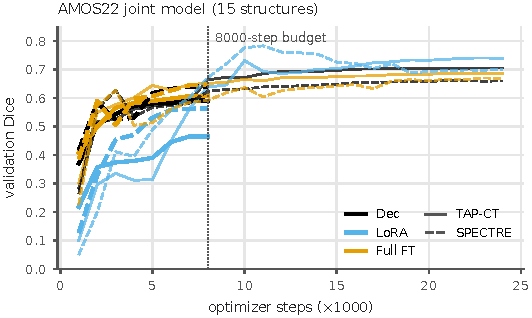
\includegraphics[width=0.62\textwidth,height=0.74\textheight,keepaspectratio]{figures/fig_seg_budget.pdf}
\caption{Validation Dice during training of the 15-structure AMOS22 joint model with the frozen decoder, LoRA and full fine-tuning, on TAP-CT (solid) and SPECTRE (dashed); thick lines stop at the shared 8000 steps, thin lines run 24\,000 steps.}
\label{fig:segbudget}
\end{figure}

\begin{figure}[H]
\centering
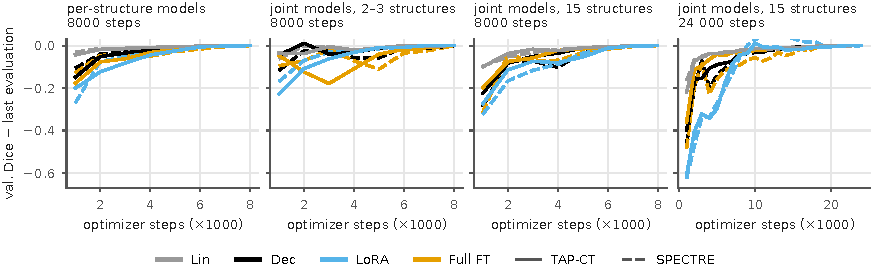
\includegraphics[width=\textwidth,height=0.74\textheight,keepaspectratio]{figures/fig_seg_convergence.pdf}
\caption{Validation Dice at each evaluation minus that at the run's last evaluation, median over the runs of each schedule group, for Lin, Dec, LoRA and Full FT on TAP-CT (solid) and SPECTRE (dashed). Every curve ends at zero by construction; a curve still rising at the right edge had not converged.}
\label{fig:segconv}
\end{figure}

\begin{figure}[H]
\centering
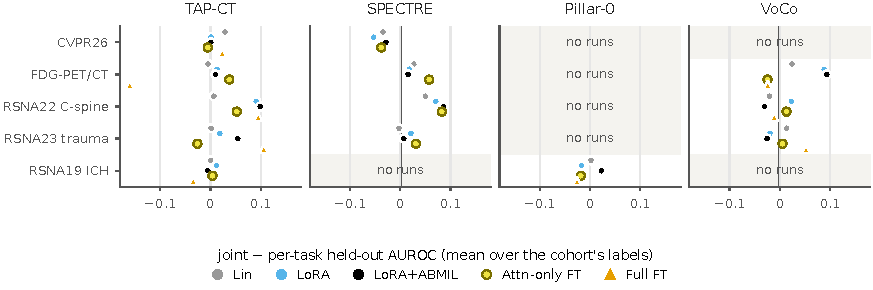
\includegraphics[width=\textwidth,height=0.74\textheight,keepaspectratio]{figures/fig_joint.pdf}
\caption{Joint minus per-task held-out AUROC, mean over the labels of each cohort, for Lin, LoRA, LoRA+ABMIL, Attn-only FT and Full FT, per backbone (SPECTRE Full FT, which did not train, is not shown). Right of zero favors one joint model per cohort.}
\label{fig:joint}
\end{figure}
\begin{figure}[H]
\centering
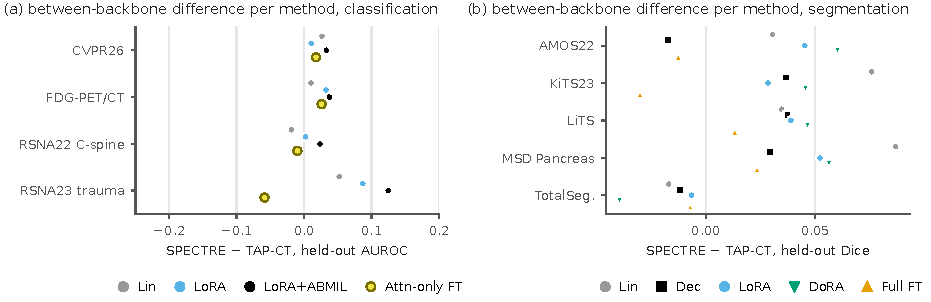
\includegraphics[width=\textwidth,height=0.74\textheight,keepaspectratio]{figures/fig_bbgap.pdf}
\caption{Between-backbone difference per method: SPECTRE minus TAP-CT held-out AUROC per cohort (a) and held-out Dice per dataset (b), on the same labels or structures and modes. SPECTRE Full FT, which did not train in classification, is not shown in (a).}
\label{fig:bbgap}
\end{figure}

\begin{figure}[H]
\centering
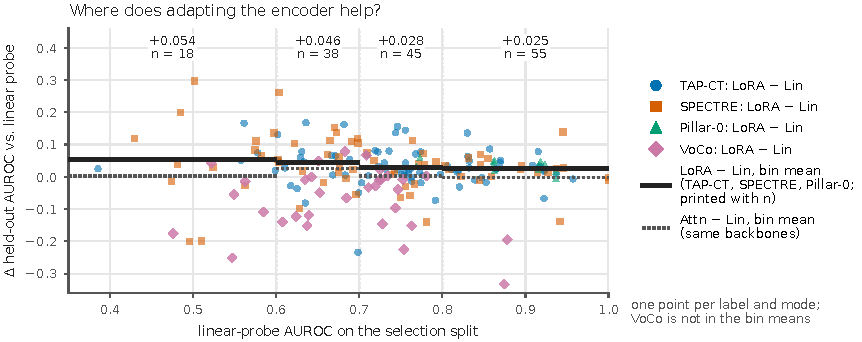
\includegraphics[width=\textwidth,height=0.74\textheight,keepaspectratio]{figures/fig_gain_vs_probe.pdf}
\caption{Where does adapting the encoder help? LoRA minus linear-probe held-out AUROC per label--mode pair against the linear probe's selection AUROC (markers: backbone), with bin means (bars, printed) and, as a negative control, the bin means of the frozen attentive probe minus the linear probe (dotted).}
\label{fig:gainprobe}
\end{figure}

\begin{table}[H]
\centering
\caption{Median over label--mode pairs of the standard deviation of the held-out probabilities per backbone and method (the did-not-train rule flags values below \numSpreadMinValue{}; applied to TAP-CT, SPECTRE and Pillar-0 only).}
\label{tab:spread}
\adjustbox{max width=\textwidth,max totalheight=0.8\textheight}{\small\setlength{\tabcolsep}{3pt}
\begin{tabular}{lccccccccccc}
\toprule
Backbone & Lin & Attn & LoRA & LoRA$_{\text{late}}$ & LoRA+ABMIL & DoRA & rsLoRA & Lin$\to$LoRA & Attn$\to$LoRA & Attn-only FT & Full FT \\
\midrule
TAP-CT & 0.227 & 0.239 & 0.239 & 0.235 & 0.233 & 0.237 & 0.167 & 0.222 & 0.225 & 0.247 & 0.170 \\
SPECTRE & 0.187 & 0.114 & 0.161 & 0.185 & 0.187 & 0.185 & 0.150 & 0.178 & 0.129 & 0.148 & \textbf{0.004}$^{\dagger}$ \\
Pillar-0 & 0.294 & 0.321 & 0.359 & 0.350 & 0.352 & 0.354 & 0.359 & 0.337 & 0.338 & 0.355 & 0.347 \\
VoCo & 0.152 & 0.023 & 0.035 & 0.032 & 0.008 & 0.030 & 0.036 & 0.150 & 0.020 & 0.041 & 0.036 \\
\bottomrule
\end{tabular}
}
\end{table}

\clearpage
\section{Seed repeats, full fine-tuning settings and compute-matched models}
\label{app:revision}

\begin{table}[H]
\centering
\caption{Held-out AUROC of the joint classification models across seeds 42, 43 and 44: mean over the cohort's labels, given as mean $\pm$ standard deviation over the seeds (their number in brackets), and the number of seeds in which the mean label difference between two methods is positive. SPECTRE Full FT, which did not train, has seed 42 only.}
\label{tab:seedscls}
\adjustbox{max width=\textwidth,max totalheight=0.8\textheight}{\scriptsize\begin{tabular}{lrrrrcc}
\toprule
Cohort & Lin & LoRA & Attn-only FT & Full FT & \begin{tabular}[b]{@{}c@{}}LoRA\\$>$ Lin\end{tabular} & \begin{tabular}[b]{@{}c@{}}Attn-only FT\\$>$ LoRA\end{tabular} \\
\midrule
\multicolumn{7}{@{}l}{\textit{TAP-CT}} \\
CVPR26 & 0.705 $\pm$ .004 (3) & 0.719 $\pm$ .016 (3) & 0.740 $\pm$ .009 (3) & 0.711 $\pm$ .029 (3) & 2/3 & 3/3 \\
FDG-PET/CT & 0.860 $\pm$ .003 (3) & 0.864 $\pm$ .008 (3) & 0.875 $\pm$ .012 (3) & 0.661 $\pm$ .130 (3) & 2/3 & 3/3 \\
RSNA23 trauma & 0.738 $\pm$ .008 (3) & 0.760 $\pm$ .002 (3) & 0.842 $\pm$ .030 (3) & 0.793 $\pm$ .157 (3) & 3/3 & 3/3 \\
RSNA22 C-spine & 0.623 $\pm$ .006 (3) & 0.659 $\pm$ .050 (3) & 0.691 $\pm$ .019 (3) & 0.695 $\pm$ .035 (3) & 2/3 & 2/3 \\
RSNA19 ICH & 0.871 $\pm$ .002 (3) & 0.896 $\pm$ .009 (3) & 0.904 $\pm$ .019 (3) & 0.836 $\pm$ .086 (3) & 3/3 & 2/3 \\
\multicolumn{7}{@{}l}{\textit{SPECTRE}} \\
CVPR26 & 0.711 $\pm$ .008 (3) & 0.741 $\pm$ .024 (3) & 0.759 $\pm$ .023 (3) & 0.575 (1) & 3/3 & 3/3 \\
FDG-PET/CT & 0.887 $\pm$ .003 (3) & 0.901 $\pm$ .000 (3) & 0.910 $\pm$ .006 (3) & 0.673 (1) & 3/3 & 3/3 \\
RSNA23 trauma & 0.792 $\pm$ .004 (3) & 0.846 $\pm$ .001 (3) & 0.834 $\pm$ .028 (3) & 0.654 (1) & 3/3 & 1/3 \\
RSNA22 C-spine & 0.592 $\pm$ .046 (3) & 0.696 $\pm$ .009 (3) & 0.683 $\pm$ .052 (3) & 0.554 (1) & 3/3 & 2/3 \\
\multicolumn{7}{@{}l}{\textit{Pillar-0}} \\
RSNA19 ICH & 0.888 $\pm$ .000 (3) & 0.916 $\pm$ .004 (3) & 0.921 $\pm$ .007 (3) & 0.894 $\pm$ .015 (3) & 3/3 & 3/3 \\
\bottomrule
\end{tabular}
}
\end{table}

\begin{table}[H]
\centering
\caption{Segmentation across seeds: held-out Dice of the joint models (AMOS22 and TotalSegmentator: 24\,000 steps), mean over structures, as in Table~\ref{tab:seedscls}.}
\label{tab:seedsseg}
\adjustbox{max width=\textwidth,max totalheight=0.8\textheight}{\footnotesize\begin{tabular}{lrrrcc}
\toprule
Dataset & Dec & LoRA & Full FT & \begin{tabular}[b]{@{}c@{}}LoRA\\$>$ Dec\end{tabular} & \begin{tabular}[b]{@{}c@{}}Full FT\\$>$ Dec\end{tabular} \\
\midrule
\multicolumn{6}{@{}l}{\textit{TAP-CT}} \\
AMOS22 & 0.675 $\pm$ .029 (3) & 0.709 $\pm$ .059 (3) & 0.680 $\pm$ .001 (3) & 2/3 & 2/3 \\
KiTS23 & 0.516 $\pm$ .003 (3) & 0.576 $\pm$ .005 (3) & 0.529 $\pm$ .014 (3) & 3/3 & 3/3 \\
LiTS & 0.715 $\pm$ .016 (3) & 0.718 $\pm$ .004 (3) & 0.717 $\pm$ .007 (3) & 2/3 & 2/3 \\
MSD Pancreas & 0.480 $\pm$ .002 (3) & 0.496 $\pm$ .009 (3) & 0.468 $\pm$ .027 (3) & 3/3 & 2/3 \\
TotalSegmentator & 0.783 $\pm$ .026 (3) & 0.773 $\pm$ .008 (3) & 0.815 $\pm$ .000 (3) & 1/3 & 3/3 \\
\multicolumn{6}{@{}l}{\textit{SPECTRE}} \\
AMOS22 & 0.658 $\pm$ .000 (3) & 0.775 $\pm$ .011 (3) & 0.669 $\pm$ .003 (3) & 3/3 & 3/3 \\
KiTS23 & 0.579 $\pm$ .010 (3) & 0.616 $\pm$ .024 (3) & 0.529 $\pm$ .015 (3) & 3/3 & 0/3 \\
LiTS & 0.741 $\pm$ .001 (3) & 0.740 $\pm$ .012 (3) & 0.707 $\pm$ .019 (3) & 1/3 & 0/3 \\
MSD Pancreas & 0.518 $\pm$ .004 (3) & 0.551 $\pm$ .008 (3) & 0.517 $\pm$ .011 (3) & 3/3 & 1/3 \\
TotalSegmentator & 0.741 $\pm$ .025 (3) & 0.752 $\pm$ .020 (3) & 0.762 $\pm$ .028 (3) & 2/3 & 3/3 \\
\bottomrule
\end{tabular}
}
\end{table}

\begin{table}[H]
\centering
\caption{Held-out AUROC of the joint classification models under the default and three alternative full fine-tuning settings, mean over the cohort's labels, next to Lin and LoRA. \textbf{Bold}: the setting with the best mean selection-split AUROC on the backbone. Grey: runs whose held-out predictions barely vary (median over labels of the standard deviation of the predicted probabilities below \numSpreadMinValue{}).}
\label{tab:fullftfix}
\adjustbox{max width=\textwidth,max totalheight=0.8\textheight}{\footnotesize\begin{tabular}{lrrrrrr}
\toprule
 & & & \multicolumn{4}{c}{Full FT} \\
\cmidrule(lr){4-7}
Cohort & Lin & LoRA & default & lower LR & layer decay & accum.\ + clip \\
\midrule
\multicolumn{7}{@{}l}{\textit{TAP-CT}} \\
CVPR26 & 0.707 & 0.733 & 0.744 & 0.730 & \textbf{0.750} & 0.685 \\
FDG-PET/CT & 0.858 & 0.866 & \textcolor{gray}{0.608} & 0.861 & \textbf{0.867} & 0.867 \\
RSNA23 trauma & 0.739 & 0.757 & 0.881 & 0.860 & \textbf{0.869} & 0.758 \\
RSNA22 C-spine & 0.626 & 0.714 & 0.732 & 0.654 & \textbf{0.618} & 0.687 \\
RSNA19 ICH & 0.871 & 0.906 & 0.854 & 0.889 & \textbf{0.917} & 0.909 \\
\multicolumn{7}{@{}l}{\textit{SPECTRE}} \\
CVPR26 & 0.702 & 0.716 & \textcolor{gray}{0.575} & 0.713 & \textbf{0.758} & \textcolor{gray}{0.511} \\
FDG-PET/CT & 0.884 & 0.901 & 0.673 & 0.884 & \textbf{0.865} & 0.883 \\
RSNA23 trauma & 0.789 & 0.846 & 0.654 & 0.793 & \textbf{0.863} & \textcolor{gray}{0.578} \\
RSNA22 C-spine & 0.629 & 0.706 & 0.554 & 0.568 & \textbf{0.700} & \textcolor{gray}{0.553} \\
\multicolumn{7}{@{}l}{\textit{Pillar-0}} \\
RSNA19 ICH & 0.888 & 0.912 & 0.878 & \textbf{0.924} & 0.920 & 0.918 \\
\bottomrule
\end{tabular}
}
\end{table}

\begin{figure}[H]
\centering
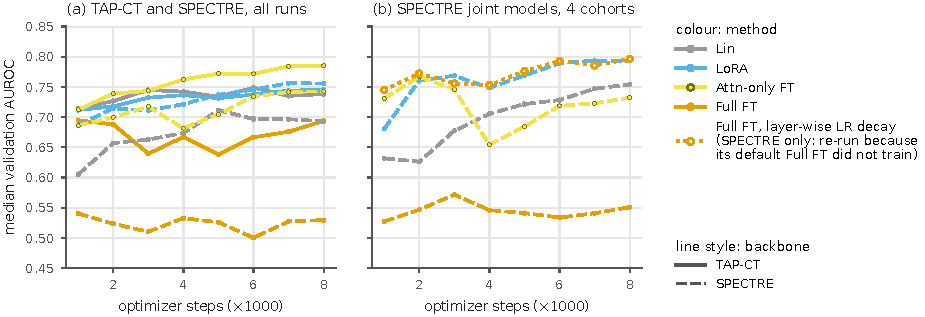
\includegraphics[width=\textwidth,height=0.74\textheight,keepaspectratio]{figures/fig_fullft_spectre.pdf}
\caption{Full fine-tuning on SPECTRE. (a) Median validation AUROC at each evaluation with the default settings, for TAP-CT and SPECTRE, over all runs of each method. (b) SPECTRE joint models on four cohorts, including Full FT with layer-wise learning-rate decay, the setting selected in Table~\ref{tab:fullftfix}; the alternative settings were run only on SPECTRE, the one backbone on which Full FT failed.}
\label{fig:fullftspectre}
\end{figure}

\begin{table}[H]
\centering
\caption{Controls for two confounds of the main comparison: rsLoRA at a quarter of the learning rate, which matches LoRA's update scale at initialization, and fine-tuning the MLP instead of the attention weights. Held-out AUROC of the joint models, mean over the cohort's labels.}
\label{tab:controls}
\adjustbox{max width=\textwidth,max totalheight=0.8\textheight}{\footnotesize\begin{tabular}{lrrrrr}
\toprule
Cohort & LoRA & rsLoRA & rsLoRA (LR$/4$) & Attn-only FT & MLP-only FT \\
\midrule
\multicolumn{6}{@{}l}{\textit{TAP-CT}} \\
CVPR26 & 0.733 & 0.722 & 0.741 & 0.739 & 0.745 \\
FDG-PET/CT & 0.866 & 0.785 & 0.855 & 0.870 & 0.866 \\
RSNA23 trauma & 0.757 & 0.684 & 0.751 & 0.833 & 0.894 \\
RSNA22 C-spine & 0.714 & 0.601 & 0.611 & 0.712 & 0.627 \\
RSNA19 ICH & 0.906 & 0.869 & 0.901 & 0.915 & 0.907 \\
\multicolumn{6}{@{}l}{\textit{SPECTRE}} \\
CVPR26 & 0.716 & 0.690 & 0.739 & 0.740 & 0.681 \\
FDG-PET/CT & 0.901 & 0.900 & 0.908 & 0.906 & 0.814 \\
RSNA23 trauma & 0.846 & 0.850 & 0.834 & 0.803 & 0.838 \\
RSNA22 C-spine & 0.706 & 0.691 & 0.672 & 0.718 & 0.626 \\
\multicolumn{6}{@{}l}{\textit{Pillar-0}} \\
RSNA19 ICH & 0.912 & 0.918 & 0.920 & 0.912 & 0.912 \\
\bottomrule
\end{tabular}
}
\end{table}

\begin{table}[H]
\centering
\caption{Joint against compute-matched per-structure segmentation: held-out Dice, mean over the 15 structures, of per-structure models trained 1600 steps (matched) or 8000 steps, and of the 24\,000-step joint model on the same structures; the difference joint $-$ matched and the number of structures where it is positive.}
\label{tab:segcm}
\adjustbox{max width=\textwidth,max totalheight=0.8\textheight}{\footnotesize\begin{tabular}{llrrrrrc}
\toprule
 & & & \multicolumn{2}{c}{per-structure} & & \multicolumn{2}{c}{joint $-$ matched} \\
\cmidrule(lr){4-5}\cmidrule(lr){7-8}
Backbone & Method & \begin{tabular}[b]{@{}c@{}}Struct.\\finished\end{tabular} & matched & 8000 steps & joint & mean & $>0$ \\
\midrule
\multicolumn{8}{@{}l}{\textit{AMOS22 (15 structures)}} \\
TAP-CT & Dec & 15 & 0.763 & 0.793 & 0.708 & $-0.055$ & 11/15 \\
TAP-CT & LoRA & 15 & 0.617 & 0.767 & 0.739 & $+0.122$ & 14/15 \\
TAP-CT & Full FT & 15 & 0.766 & 0.805 & 0.681 & $-0.085$ & 12/15 \\
SPECTRE & Dec & 15 & 0.760 & 0.808 & 0.658 & $-0.101$ & 6/15 \\
SPECTRE & LoRA & 15 & 0.648 & 0.812 & 0.784 & $+0.136$ & 14/15 \\
SPECTRE & Full FT & 15 & 0.793 & 0.792 & 0.669 & $-0.123$ & 5/15 \\
\multicolumn{8}{@{}l}{\textit{TotalSegmentator (15 structures)}} \\
TAP-CT & Dec & 15 & 0.783 & 0.843 & 0.798 & $+0.015$ & 13/15 \\
TAP-CT & LoRA & 15 & 0.657 & 0.819 & 0.776 & $+0.119$ & 14/15 \\
TAP-CT & Full FT & 15 & 0.803 & 0.832 & 0.815 & $+0.012$ & 14/15 \\
SPECTRE & Dec & 15 & 0.806 & 0.848 & 0.770 & $-0.037$ & 6/15 \\
SPECTRE & LoRA & 15 & 0.691 & 0.848 & 0.733 & $+0.042$ & 11/15 \\
SPECTRE & Full FT & 15 & 0.819 & 0.838 & 0.795 & $-0.024$ & 10/15 \\
\bottomrule
\end{tabular}
}
\end{table}

\begin{table}[H]
\centering
\caption{From-scratch control: TAP-CT architecture with a randomly initialised encoder, trained as the Full FT joint model, next to Full FT and Dec, per dataset (held-out Dice, mean over structures).}
\label{tab:scratch}
\adjustbox{max width=\textwidth,max totalheight=0.8\textheight}{\footnotesize\begin{tabular}{@{}lccccc@{}}
\toprule
Dataset (structures) & From scratch & Dec & Full FT & Scratch $-$ Dec & Scratch $-$ Full FT \\
\midrule
AMOS22 (15) & 0.496 & 0.708 & 0.681 & -0.212 & -0.185 \\
KiTS23 (3) & 0.400 & 0.514 & 0.519 & -0.114 & -0.120 \\
LiTS (2) & 0.612 & 0.699 & 0.715 & -0.087 & -0.103 \\
MSD Pancreas (2) & 0.308 & 0.480 & 0.487 & -0.172 & -0.180 \\
TotalSegmentator (15) & 0.579 & 0.798 & 0.815 & -0.219 & -0.236 \\
\bottomrule
\end{tabular}
}
\end{table}

\clearpage
\section{Per-cohort, per-label and per-structure results}
\label{app:perlabel}
\begin{table}[H]
\centering
\caption{Classification: held-out AUROC, mean over the labels of each cohort (number of labels in brackets), per backbone, training mode and method. Within each row, \textbf{bold} is the best and \underline{underlined} the second-best method. A \colorbox{modebest}{shaded} cell marks the better of per-task and joint training for that method, backbone and cohort. SPECTRE Full FT did not train with the default setting (Section~\ref{sec:clsres}). VoCo was run on three cohorts.}
\label{tab:cls}
\adjustbox{max width=\textwidth,max totalheight=0.8\textheight}{\footnotesize\setlength{\tabcolsep}{3pt}
\begin{tabular}{lllccccccccccc}
\toprule
Cohort (labels) & Backbone & Mode & Lin & Attn & LoRA & LoRA$_{\text{late}}$ & \begin{tabular}[b]{@{}c@{}}LoRA+\\ABMIL\end{tabular} & DoRA & rsLoRA & \begin{tabular}[b]{@{}c@{}}Lin$\to$\\LoRA\end{tabular} & \begin{tabular}[b]{@{}c@{}}Attn$\to$\\LoRA\end{tabular} & \begin{tabular}[b]{@{}c@{}}Attn-only\\FT\end{tabular} & \begin{tabular}[b]{@{}c@{}}Full\\FT\end{tabular} \\
\midrule
CVPR26 (17) & TAP-CT & per-task & 0.677 & 0.718 & \underline{0.732} & 0.704 & 0.728 & 0.717 & \cellcolor{modebest}0.724 & \cellcolor{modebest}0.697 & 0.707 & \cellcolor{modebest}\textbf{0.744} & 0.720 \\
 &  & joint & \cellcolor{modebest}0.707 & \cellcolor{modebest}0.720 & \cellcolor{modebest}0.733 & \cellcolor{modebest}0.726 & \cellcolor{modebest}0.729 & \cellcolor{modebest}0.733 & 0.722 & 0.695 & \cellcolor{modebest}0.708 & \underline{0.739} & \cellcolor{modebest}\textbf{0.744} \\
\addlinespace[2pt]
CVPR26 (17) & SPECTRE & per-task & \cellcolor{modebest}0.736 & 0.725 & \cellcolor{modebest}0.769 & \cellcolor{modebest}0.769 & \cellcolor{modebest}\underline{0.776} & \cellcolor{modebest}0.766 & \cellcolor{modebest}0.768 & \cellcolor{modebest}0.769 & \cellcolor{modebest}0.765 & \cellcolor{modebest}\textbf{0.778} & \cellcolor{modebest}0.627 \\
 &  & joint & 0.702 & \cellcolor{modebest}0.738 & 0.716 & 0.731 & \textbf{0.747} & 0.731 & 0.690 & \underline{0.744} & 0.728 & 0.740 & 0.575 \\
\addlinespace[2pt]
FDG (4) & TAP-CT & per-task & \cellcolor{modebest}0.863 & 0.836 & 0.852 & \cellcolor{modebest}\textbf{0.868} & 0.839 & 0.847 & \cellcolor{modebest}0.817 & \cellcolor{modebest}\underline{0.866} & 0.856 & 0.832 & \cellcolor{modebest}0.769 \\
 &  & joint & 0.858 & \cellcolor{modebest}0.860 & \cellcolor{modebest}\underline{0.866} & 0.864 & \cellcolor{modebest}0.849 & \cellcolor{modebest}0.858 & 0.785 & 0.860 & \cellcolor{modebest}0.862 & \cellcolor{modebest}\textbf{0.870} & 0.608 \\
\addlinespace[2pt]
FDG (4) & SPECTRE & per-task & 0.857 & 0.862 & 0.882 & 0.879 & 0.874 & \textbf{0.892} & 0.872 & \cellcolor{modebest}\underline{0.887} & 0.867 & 0.848 & 0.617 \\
 &  & joint & \cellcolor{modebest}0.884 & \cellcolor{modebest}0.880 & \cellcolor{modebest}\underline{0.901} & \cellcolor{modebest}0.888 & \cellcolor{modebest}0.889 & \cellcolor{modebest}0.900 & \cellcolor{modebest}0.900 & 0.884 & \cellcolor{modebest}0.884 & \cellcolor{modebest}\textbf{0.906} & \cellcolor{modebest}0.673 \\
\addlinespace[2pt]
FDG (4) & VoCo & per-task & \underline{0.720} & 0.685 & 0.512 & \cellcolor{modebest}0.671 & 0.562 & \cellcolor{modebest}0.669 & \cellcolor{modebest}0.598 & \textbf{0.736} & \cellcolor{modebest}0.591 & \cellcolor{modebest}0.665 & \cellcolor{modebest}0.606 \\
 &  & joint & \cellcolor{modebest}\underline{0.745} & \cellcolor{modebest}0.739 & \cellcolor{modebest}0.600 & 0.506 & \cellcolor{modebest}0.655 & 0.564 & 0.527 & \cellcolor{modebest}\textbf{0.750} & 0.520 & 0.641 & 0.582 \\
\addlinespace[2pt]
RSNA22 (8) & TAP-CT & per-task & 0.619 & \cellcolor{modebest}0.625 & 0.623 & 0.608 & 0.613 & \underline{0.641} & \cellcolor{modebest}0.635 & 0.606 & \cellcolor{modebest}0.629 & \textbf{0.660} & 0.637 \\
 &  & joint & \cellcolor{modebest}0.626 & 0.624 & \cellcolor{modebest}\underline{0.714} & \cellcolor{modebest}0.706 & \cellcolor{modebest}0.713 & \cellcolor{modebest}0.680 & 0.601 & \cellcolor{modebest}0.624 & 0.620 & \cellcolor{modebest}0.712 & \cellcolor{modebest}\textbf{0.732} \\
\addlinespace[2pt]
RSNA22 (8) & SPECTRE & per-task & 0.579 & 0.591 & 0.635 & \cellcolor{modebest}\textbf{0.654} & \underline{0.644} & 0.619 & 0.638 & 0.615 & 0.591 & 0.635 & \cellcolor{modebest}0.566 \\
 &  & joint & \cellcolor{modebest}0.629 & \cellcolor{modebest}0.601 & \cellcolor{modebest}0.706 & 0.644 & \cellcolor{modebest}\textbf{0.730} & \cellcolor{modebest}0.692 & \cellcolor{modebest}0.691 & \cellcolor{modebest}0.670 & \cellcolor{modebest}0.611 & \cellcolor{modebest}\underline{0.718} & 0.554 \\
\addlinespace[2pt]
RSNA22 (8) & VoCo & per-task & \cellcolor{modebest}\underline{0.606} & 0.508 & 0.537 & \cellcolor{modebest}0.551 & \cellcolor{modebest}0.596 & 0.561 & \cellcolor{modebest}\textbf{0.617} & 0.602 & 0.521 & 0.576 & \cellcolor{modebest}0.605 \\
 &  & joint & 0.586 & \cellcolor{modebest}0.548 & \cellcolor{modebest}0.560 & 0.550 & 0.565 & \cellcolor{modebest}0.589 & 0.578 & \cellcolor{modebest}\textbf{0.619} & \cellcolor{modebest}0.527 & \cellcolor{modebest}0.589 & \underline{0.593} \\
\addlinespace[2pt]
RSNA23 (4) & TAP-CT & per-task & 0.737 & 0.718 & 0.739 & \cellcolor{modebest}0.756 & 0.703 & 0.752 & \cellcolor{modebest}0.725 & 0.738 & 0.716 & \cellcolor{modebest}\textbf{0.859} & \underline{0.775} \\
 &  & joint & \cellcolor{modebest}0.739 & \cellcolor{modebest}0.738 & \cellcolor{modebest}0.757 & 0.744 & \cellcolor{modebest}0.758 & \cellcolor{modebest}0.768 & 0.684 & \cellcolor{modebest}0.746 & \cellcolor{modebest}0.758 & \underline{0.833} & \cellcolor{modebest}\textbf{0.881} \\
\addlinespace[2pt]
RSNA23 (4) & SPECTRE & per-task & \cellcolor{modebest}0.791 & 0.778 & 0.824 & 0.832 & \textbf{0.852} & \cellcolor{modebest}\underline{0.842} & 0.836 & 0.825 & 0.798 & 0.772 & 0.624 \\
 &  & joint & 0.789 & \cellcolor{modebest}0.788 & \cellcolor{modebest}0.846 & \cellcolor{modebest}0.835 & \cellcolor{modebest}\textbf{0.859} & 0.838 & \cellcolor{modebest}\underline{0.850} & \cellcolor{modebest}0.827 & \cellcolor{modebest}0.810 & \cellcolor{modebest}0.803 & \cellcolor{modebest}0.654 \\
\addlinespace[2pt]
RSNA23 (4) & VoCo & per-task & 0.617 & \cellcolor{modebest}\underline{0.625} & \cellcolor{modebest}0.622 & 0.601 & \cellcolor{modebest}0.595 & \cellcolor{modebest}0.611 & \cellcolor{modebest}0.608 & \cellcolor{modebest}\textbf{0.631} & 0.569 & 0.588 & 0.596 \\
 &  & joint & \cellcolor{modebest}0.631 & 0.616 & 0.603 & \cellcolor{modebest}0.627 & 0.570 & 0.583 & 0.607 & 0.626 & \cellcolor{modebest}\underline{0.635} & \cellcolor{modebest}0.593 & \cellcolor{modebest}\textbf{0.648} \\
\addlinespace[2pt]
ICH (6) & TAP-CT & per-task & 0.870 & 0.873 & 0.894 & 0.894 & \cellcolor{modebest}0.891 & \underline{0.897} & \cellcolor{modebest}0.870 & \cellcolor{modebest}0.877 & \cellcolor{modebest}0.878 & \textbf{0.911} & \cellcolor{modebest}0.888 \\
 &  & joint & \cellcolor{modebest}0.871 & \cellcolor{modebest}0.877 & \cellcolor{modebest}\underline{0.906} & \cellcolor{modebest}0.895 & 0.886 & 0.897 & 0.869 & 0.868 & 0.876 & \cellcolor{modebest}\textbf{0.915} & 0.854 \\
\addlinespace[2pt]
ICH (6) & Pillar-0 & per-task & 0.886 & 0.884 & \cellcolor{modebest}\underline{0.929} & \cellcolor{modebest}0.914 & 0.902 & \cellcolor{modebest}\textbf{0.931} & \cellcolor{modebest}0.920 & \cellcolor{modebest}0.912 & \cellcolor{modebest}0.903 & \cellcolor{modebest}\textbf{0.931} & \cellcolor{modebest}0.904 \\
 &  & joint & \cellcolor{modebest}0.888 & \cellcolor{modebest}0.888 & 0.912 & 0.892 & \cellcolor{modebest}\textbf{0.925} & 0.912 & \underline{0.918} & 0.905 & 0.898 & 0.912 & 0.878 \\
\addlinespace[2pt]
\bottomrule
\end{tabular}
}
\end{table}
\begin{table}[H]
\centering
\caption{Segmentation: held-out Dice, mean over the structures of each dataset (number of structures in brackets), per backbone, training mode and method; -- marks methods not run per structure on TotalSegmentator. Within each row, \textbf{bold} is the best and \underline{underlined} the second-best method. A \colorbox{modebest}{shaded} cell marks the better of per-structure and joint training for that method, backbone and dataset. The AMOS22 and TotalSegmentator joint models train 24\,000 steps. VoCo's Lin reads stage-4 tokens at a stride of 32 voxels.}
\label{tab:seg}
\adjustbox{max width=\textwidth,max totalheight=0.8\textheight}{\footnotesize\begin{tabular}{lllccccccc}
\toprule
Dataset (structures) & Backbone & Mode & Lin & Dec & LoRA & LoRA$_{\text{late}}$ & DoRA & Full FT & Dec$\to$LoRA \\
\midrule
AMOS22 (15) & TAP-CT & per-task & \cellcolor{modebest}0.658 & \cellcolor{modebest}\underline{0.793} & \cellcolor{modebest}0.767 & \cellcolor{modebest}0.764 & \cellcolor{modebest}0.761 & \cellcolor{modebest}\textbf{0.805} & \cellcolor{modebest}0.791 \\
 &  & joint & 0.646 & \underline{0.708} & \textbf{0.739} & 0.698 & \underline{0.708} & 0.681 & 0.656 \\
\addlinespace[2pt]
AMOS22 (15) & SPECTRE & per-task & \cellcolor{modebest}0.683 & \cellcolor{modebest}0.808 & \cellcolor{modebest}\underline{0.812} & \cellcolor{modebest}0.806 & \cellcolor{modebest}\textbf{0.814} & \cellcolor{modebest}0.792 & \cellcolor{modebest}\textbf{0.814} \\
 &  & joint & 0.682 & 0.658 & \textbf{0.784} & 0.764 & \underline{0.775} & 0.669 & 0.664 \\
\addlinespace[2pt]
AMOS22 (15) & VoCo & per-task & \cellcolor{modebest}0.041 & \cellcolor{modebest}\underline{0.805} & \cellcolor{modebest}0.782 & \cellcolor{modebest}0.783 & \cellcolor{modebest}0.783 & \cellcolor{modebest}\textbf{0.818} & \cellcolor{modebest}0.799 \\
 &  & joint & 0.038 & 0.739 & \underline{0.762} & 0.758 & \textbf{0.764} & 0.752 & 0.736 \\
\addlinespace[2pt]
KiTS23 (3) & TAP-CT & per-task & \cellcolor{modebest}0.531 & \cellcolor{modebest}0.584 & 0.563 & \cellcolor{modebest}0.567 & \cellcolor{modebest}0.563 & \cellcolor{modebest}\textbf{0.588} & \cellcolor{modebest}\underline{0.587} \\
 &  & joint & 0.430 & 0.514 & \cellcolor{modebest}\textbf{0.582} & 0.556 & \underline{0.560} & 0.519 & 0.500 \\
\addlinespace[2pt]
KiTS23 (3) & SPECTRE & per-task & \cellcolor{modebest}0.583 & \cellcolor{modebest}0.599 & \cellcolor{modebest}0.613 & \cellcolor{modebest}\underline{0.617} & \cellcolor{modebest}\textbf{0.622} & \cellcolor{modebest}0.528 & \cellcolor{modebest}0.603 \\
 &  & joint & 0.530 & 0.572 & \underline{0.588} & \underline{0.588} & \textbf{0.593} & 0.519 & 0.570 \\
\addlinespace[2pt]
KiTS23 (3) & VoCo & per-task & 0.017 & \cellcolor{modebest}\underline{0.519} & 0.501 & 0.500 & 0.493 & \cellcolor{modebest}\textbf{0.564} & \cellcolor{modebest}0.481 \\
 &  & joint & \cellcolor{modebest}0.037 & 0.465 & 0.501 & \cellcolor{modebest}\textbf{0.516} & \cellcolor{modebest}\underline{0.507} & 0.481 & 0.452 \\
\addlinespace[2pt]
LiTS (2) & TAP-CT & per-task & \cellcolor{modebest}0.659 & \cellcolor{modebest}0.709 & \cellcolor{modebest}\textbf{0.716} & 0.709 & \cellcolor{modebest}\underline{0.714} & 0.710 & \cellcolor{modebest}\underline{0.714} \\
 &  & joint & 0.656 & 0.699 & \underline{0.715} & \cellcolor{modebest}\textbf{0.721} & 0.692 & \cellcolor{modebest}\underline{0.715} & 0.703 \\
\addlinespace[2pt]
LiTS (2) & SPECTRE & per-task & 0.688 & \underline{0.741} & \cellcolor{modebest}\textbf{0.756} & 0.723 & \cellcolor{modebest}\textbf{0.756} & \cellcolor{modebest}0.739 & 0.729 \\
 &  & joint & \cellcolor{modebest}0.696 & \cellcolor{modebest}0.742 & \textbf{0.753} & \cellcolor{modebest}0.736 & \underline{0.743} & 0.713 & \cellcolor{modebest}\underline{0.743} \\
\addlinespace[2pt]
LiTS (2) & VoCo & per-task & 0.342 & \cellcolor{modebest}\underline{0.733} & 0.692 & 0.694 & 0.688 & \cellcolor{modebest}\textbf{0.748} & 0.720 \\
 &  & joint & \cellcolor{modebest}0.345 & \underline{0.732} & \cellcolor{modebest}0.720 & \cellcolor{modebest}0.710 & \cellcolor{modebest}0.718 & \textbf{0.737} & \cellcolor{modebest}0.726 \\
\addlinespace[2pt]
MSD Pancreas (2) & TAP-CT & per-task & \cellcolor{modebest}0.427 & \cellcolor{modebest}0.491 & \underline{0.504} & \cellcolor{modebest}0.501 & \cellcolor{modebest}0.502 & \cellcolor{modebest}\textbf{0.512} & \cellcolor{modebest}0.495 \\
 &  & joint & 0.334 & 0.480 & \cellcolor{modebest}\textbf{0.505} & 0.492 & \underline{0.493} & 0.487 & 0.468 \\
\addlinespace[2pt]
MSD Pancreas (2) & SPECTRE & per-task & \cellcolor{modebest}0.475 & \cellcolor{modebest}0.516 & \cellcolor{modebest}\textbf{0.563} & \cellcolor{modebest}0.538 & \cellcolor{modebest}\underline{0.557} & 0.516 & 0.518 \\
 &  & joint & 0.459 & 0.514 & \textbf{0.550} & 0.529 & \textbf{0.550} & \cellcolor{modebest}\underline{0.530} & \cellcolor{modebest}0.520 \\
\addlinespace[2pt]
MSD Pancreas (2) & VoCo & per-task & 0.000 & \cellcolor{modebest}\textbf{0.569} & 0.539 & 0.545 & 0.541 & \cellcolor{modebest}\underline{0.566} & 0.558 \\
 &  & joint & 0.000 & 0.559 & \cellcolor{modebest}0.552 & 0.545 & \cellcolor{modebest}0.552 & \underline{0.560} & \cellcolor{modebest}\textbf{0.561} \\
\addlinespace[2pt]
TotalSegmentator (15) & TAP-CT & per-task & \cellcolor{modebest}0.747 & \cellcolor{modebest}\textbf{0.843} & \cellcolor{modebest}0.819 & -- & -- & \cellcolor{modebest}\underline{0.832} & -- \\
 &  & joint & 0.740 & \underline{0.798} & 0.776 & 0.776 & 0.776 & \textbf{0.815} & 0.790 \\
\addlinespace[2pt]
TotalSegmentator (15) & SPECTRE & per-task & \cellcolor{modebest}0.731 & \cellcolor{modebest}\textbf{0.848} & \cellcolor{modebest}\textbf{0.848} & -- & -- & \cellcolor{modebest}\underline{0.838} & -- \\
 &  & joint & 0.722 & 0.770 & 0.733 & 0.752 & 0.736 & \textbf{0.795} & \underline{0.772} \\
\addlinespace[2pt]
TotalSegmentator (15) & VoCo & per-task & \cellcolor{modebest}0.055 & \cellcolor{modebest}\underline{0.822} & \cellcolor{modebest}0.771 & -- & -- & \cellcolor{modebest}\textbf{0.838} & -- \\
 &  & joint & 0.047 & \underline{0.732} & 0.705 & 0.697 & 0.709 & \textbf{0.750} & 0.723 \\
\addlinespace[2pt]
\bottomrule
\end{tabular}
}
\end{table}

\begin{table}[H]
\centering
\caption{Held-out AUROC as in Table~\ref{tab:cls}, with the longer CVPR26 joint schedule (26\,000 steps) as an extra row. \textbf{Bold}: best, \underline{underlined}: second best of the row; \colorbox{modebest}{shaded}: the better of per-task and joint training (8000 steps).}
\label{tab:ladder}
\adjustbox{max width=\textwidth,max totalheight=0.8\textheight}{\footnotesize\begin{tabular}{lllccccccccccc}
\toprule
Cohort & Backbone & Mode (labels) & Lin & Attn & LoRA & LoRA$_{\text{late}}$ & LoRA+ABMIL & DoRA & rsLoRA & Lin$\to$LoRA & Attn$\to$LoRA & Attn-only FT & Full FT \\
\midrule
CVPR26 & TAP-CT & per-task (17) & 0.677 & 0.718 & \underline{0.732} & 0.704 & 0.728 & 0.717 & \cellcolor{modebest}0.724 & \cellcolor{modebest}0.697 & 0.707 & \cellcolor{modebest}\textbf{0.744} & 0.720 \\
CVPR26 & TAP-CT & joint (17) & \cellcolor{modebest}0.707 & \cellcolor{modebest}0.720 & \cellcolor{modebest}0.733 & \cellcolor{modebest}0.726 & \cellcolor{modebest}0.729 & \cellcolor{modebest}0.733 & 0.722 & 0.695 & \cellcolor{modebest}0.708 & \underline{0.739} & \cellcolor{modebest}\textbf{0.744} \\
CVPR26 & TAP-CT & joint (26\,000 steps) (17) & 0.693 & 0.722 & 0.692 & \underline{0.728} & 0.727 & 0.720 & 0.701 & 0.698 & 0.726 & \textbf{0.756} & 0.650 \\
\addlinespace[2pt]
CVPR26 & SPECTRE & per-task (17) & \cellcolor{modebest}0.736 & 0.725 & \cellcolor{modebest}0.769 & \cellcolor{modebest}0.769 & \cellcolor{modebest}\underline{0.776} & \cellcolor{modebest}0.766 & \cellcolor{modebest}0.768 & \cellcolor{modebest}0.769 & \cellcolor{modebest}0.765 & \cellcolor{modebest}\textbf{0.778} & \cellcolor{modebest}0.627 \\
CVPR26 & SPECTRE & joint (17) & 0.702 & \cellcolor{modebest}0.738 & 0.716 & 0.731 & \textbf{0.747} & 0.731 & 0.690 & \underline{0.744} & 0.728 & 0.740 & 0.575 \\
CVPR26 & SPECTRE & joint (26\,000 steps) (17) & 0.744 & 0.713 & 0.755 & \underline{0.762} & 0.760 & 0.752 & \textbf{0.763} & 0.746 & 0.758 & 0.756 & 0.574 \\
\addlinespace[2pt]
FDG-PET/CT & TAP-CT & per-task (4) & \cellcolor{modebest}0.863 & 0.836 & 0.852 & \cellcolor{modebest}\textbf{0.868} & 0.839 & 0.847 & \cellcolor{modebest}0.817 & \cellcolor{modebest}\underline{0.866} & 0.856 & 0.832 & \cellcolor{modebest}0.769 \\
FDG-PET/CT & TAP-CT & joint (4) & 0.858 & \cellcolor{modebest}0.860 & \cellcolor{modebest}\underline{0.866} & 0.864 & \cellcolor{modebest}0.849 & \cellcolor{modebest}0.858 & 0.785 & 0.860 & \cellcolor{modebest}0.862 & \cellcolor{modebest}\textbf{0.870} & 0.608 \\
\addlinespace[2pt]
FDG-PET/CT & SPECTRE & per-task (4) & 0.857 & 0.862 & 0.882 & 0.879 & 0.874 & \textbf{0.892} & 0.872 & \cellcolor{modebest}\underline{0.887} & 0.867 & 0.848 & 0.617 \\
FDG-PET/CT & SPECTRE & joint (4) & \cellcolor{modebest}0.884 & \cellcolor{modebest}0.880 & \cellcolor{modebest}\underline{0.901} & \cellcolor{modebest}0.888 & \cellcolor{modebest}0.889 & \cellcolor{modebest}0.900 & \cellcolor{modebest}0.900 & 0.884 & \cellcolor{modebest}0.884 & \cellcolor{modebest}\textbf{0.906} & \cellcolor{modebest}0.673 \\
\addlinespace[2pt]
FDG-PET/CT & VoCo & per-task (4) & \underline{0.720} & 0.685 & 0.512 & \cellcolor{modebest}0.671 & 0.562 & \cellcolor{modebest}0.669 & \cellcolor{modebest}0.598 & \textbf{0.736} & \cellcolor{modebest}0.591 & \cellcolor{modebest}0.665 & \cellcolor{modebest}0.606 \\
FDG-PET/CT & VoCo & joint (4) & \cellcolor{modebest}\underline{0.745} & \cellcolor{modebest}0.739 & \cellcolor{modebest}0.600 & 0.506 & \cellcolor{modebest}0.655 & 0.564 & 0.527 & \cellcolor{modebest}\textbf{0.750} & 0.520 & 0.641 & 0.582 \\
\addlinespace[2pt]
RSNA 2022 C-spine & TAP-CT & per-task (8) & 0.619 & \cellcolor{modebest}0.625 & 0.623 & 0.608 & 0.613 & \underline{0.641} & \cellcolor{modebest}0.635 & 0.606 & \cellcolor{modebest}0.629 & \textbf{0.660} & 0.637 \\
RSNA 2022 C-spine & TAP-CT & joint (8) & \cellcolor{modebest}0.626 & 0.624 & \cellcolor{modebest}\underline{0.714} & \cellcolor{modebest}0.706 & \cellcolor{modebest}0.713 & \cellcolor{modebest}0.680 & 0.601 & \cellcolor{modebest}0.624 & 0.620 & \cellcolor{modebest}0.712 & \cellcolor{modebest}\textbf{0.732} \\
\addlinespace[2pt]
RSNA 2022 C-spine & SPECTRE & per-task (8) & 0.579 & 0.591 & 0.635 & \cellcolor{modebest}\textbf{0.654} & \underline{0.644} & 0.619 & 0.638 & 0.615 & 0.591 & 0.635 & \cellcolor{modebest}0.566 \\
RSNA 2022 C-spine & SPECTRE & joint (8) & \cellcolor{modebest}0.629 & \cellcolor{modebest}0.601 & \cellcolor{modebest}0.706 & 0.644 & \cellcolor{modebest}\textbf{0.730} & \cellcolor{modebest}0.692 & \cellcolor{modebest}0.691 & \cellcolor{modebest}0.670 & \cellcolor{modebest}0.611 & \cellcolor{modebest}\underline{0.718} & 0.554 \\
\addlinespace[2pt]
RSNA 2022 C-spine & VoCo & per-task (8) & \cellcolor{modebest}\underline{0.606} & 0.508 & 0.537 & \cellcolor{modebest}0.551 & \cellcolor{modebest}0.596 & 0.561 & \cellcolor{modebest}\textbf{0.617} & 0.602 & 0.521 & 0.576 & \cellcolor{modebest}0.605 \\
RSNA 2022 C-spine & VoCo & joint (8) & 0.586 & \cellcolor{modebest}0.548 & \cellcolor{modebest}0.560 & 0.550 & 0.565 & \cellcolor{modebest}0.589 & 0.578 & \cellcolor{modebest}\textbf{0.619} & \cellcolor{modebest}0.527 & \cellcolor{modebest}0.589 & \underline{0.593} \\
\addlinespace[2pt]
RSNA 2023 trauma & TAP-CT & per-task (4) & 0.737 & 0.718 & 0.739 & \cellcolor{modebest}0.756 & 0.703 & 0.752 & \cellcolor{modebest}0.725 & 0.738 & 0.716 & \cellcolor{modebest}\textbf{0.859} & \underline{0.775} \\
RSNA 2023 trauma & TAP-CT & joint (4) & \cellcolor{modebest}0.739 & \cellcolor{modebest}0.738 & \cellcolor{modebest}0.757 & 0.744 & \cellcolor{modebest}0.758 & \cellcolor{modebest}0.768 & 0.684 & \cellcolor{modebest}0.746 & \cellcolor{modebest}0.758 & \underline{0.833} & \cellcolor{modebest}\textbf{0.881} \\
\addlinespace[2pt]
RSNA 2023 trauma & SPECTRE & per-task (4) & \cellcolor{modebest}0.791 & 0.778 & 0.824 & 0.832 & \textbf{0.852} & \cellcolor{modebest}\underline{0.842} & 0.836 & 0.825 & 0.798 & 0.772 & 0.624 \\
RSNA 2023 trauma & SPECTRE & joint (4) & 0.789 & \cellcolor{modebest}0.788 & \cellcolor{modebest}0.846 & \cellcolor{modebest}0.835 & \cellcolor{modebest}\textbf{0.859} & 0.838 & \cellcolor{modebest}\underline{0.850} & \cellcolor{modebest}0.827 & \cellcolor{modebest}0.810 & \cellcolor{modebest}0.803 & \cellcolor{modebest}0.654 \\
\addlinespace[2pt]
RSNA 2023 trauma & VoCo & per-task (4) & 0.617 & \cellcolor{modebest}\underline{0.625} & \cellcolor{modebest}0.622 & 0.601 & \cellcolor{modebest}0.595 & \cellcolor{modebest}0.611 & \cellcolor{modebest}0.608 & \cellcolor{modebest}\textbf{0.631} & 0.569 & 0.588 & 0.596 \\
RSNA 2023 trauma & VoCo & joint (4) & \cellcolor{modebest}0.631 & 0.616 & 0.603 & \cellcolor{modebest}0.627 & 0.570 & 0.583 & 0.607 & 0.626 & \cellcolor{modebest}\underline{0.635} & \cellcolor{modebest}0.593 & \cellcolor{modebest}\textbf{0.648} \\
\addlinespace[2pt]
RSNA 2019 ICH & TAP-CT & per-task (6) & 0.870 & 0.873 & 0.894 & 0.894 & \cellcolor{modebest}0.891 & \underline{0.897} & \cellcolor{modebest}0.870 & \cellcolor{modebest}0.877 & \cellcolor{modebest}0.878 & \textbf{0.911} & \cellcolor{modebest}0.888 \\
RSNA 2019 ICH & TAP-CT & joint (6) & \cellcolor{modebest}0.871 & \cellcolor{modebest}0.877 & \cellcolor{modebest}\underline{0.906} & \cellcolor{modebest}0.895 & 0.886 & 0.897 & 0.869 & 0.868 & 0.876 & \cellcolor{modebest}\textbf{0.915} & 0.854 \\
\addlinespace[2pt]
RSNA 2019 ICH & Pillar-0 & per-task (6) & 0.886 & 0.884 & \cellcolor{modebest}\underline{0.929} & \cellcolor{modebest}0.914 & 0.902 & \cellcolor{modebest}\textbf{0.931} & \cellcolor{modebest}0.920 & \cellcolor{modebest}0.912 & \cellcolor{modebest}0.903 & \cellcolor{modebest}\textbf{0.931} & \cellcolor{modebest}0.904 \\
RSNA 2019 ICH & Pillar-0 & joint (6) & \cellcolor{modebest}0.888 & \cellcolor{modebest}0.888 & 0.912 & 0.892 & \cellcolor{modebest}\textbf{0.925} & 0.912 & \underline{0.918} & 0.905 & 0.898 & 0.912 & 0.878 \\
\addlinespace[2pt]
\bottomrule
\end{tabular}
}
\end{table}

\clearpage
\begin{center}\begin{minipage}{\textwidth}\centering\footnotesize\textit{CVPR26, TAP-CT}\\[2pt]\adjustbox{max width=\textwidth}{\begin{tabular}{lccccccccccc}
\toprule
Label & Lin & Attn & LoRA & LoRA$_{\text{late}}$ & LoRA+ABMIL & DoRA & rsLoRA & Lin$\to$LoRA & Attn$\to$LoRA & Attn-only FT & Full FT \\
\midrule
\multicolumn{12}{l}{\textit{TAP-CT, per-task}} \\
adrenal\_hyperplasia & 0.80 [0.62,0.95] & 0.84 [0.68,0.97] & 0.80 [0.62,0.96] & 0.79 [0.62,0.95] & 0.81 [0.64,0.95] & 0.77 [0.59,0.92] & 0.79 [0.60,0.94] & 0.80 [0.62,0.95] & 0.82 [0.67,0.95] & 0.84 [0.68,0.97] & 0.87 [0.72,0.98] \\
ascites & 0.78 [0.60,0.92] & 0.84 [0.67,0.97] & 0.77 [0.59,0.92] & 0.74 [0.55,0.90] & 0.78 [0.61,0.92] & 0.71 [0.50,0.87] & 0.77 [0.60,0.93] & 0.76 [0.58,0.92] & 0.75 [0.56,0.92] & 0.68 [0.47,0.85] & 0.82 [0.66,0.95] \\
atherosclerosis & 0.75 [0.57,0.90] & 0.87 [0.73,0.97] & 0.89 [0.76,0.97] & 0.83 [0.68,0.96] & 0.83 [0.68,0.95] & 0.84 [0.68,0.96] & 0.86 [0.71,0.97] & 0.75 [0.56,0.90] & 0.86 [0.71,0.97] & 0.81 [0.64,0.93] & 0.88 [0.74,0.97] \\
cholecystitis & 0.73 [0.56,0.88] & 0.78 [0.62,0.92] & 0.74 [0.55,0.90] & 0.69 [0.49,0.85] & 0.73 [0.54,0.89] & 0.75 [0.60,0.90] & 0.74 [0.56,0.89] & 0.75 [0.56,0.91] & 0.72 [0.56,0.88] & 0.77 [0.60,0.91] & 0.74 [0.57,0.89] \\
colorectal\_cancer & 0.56 [0.33,0.77] & 0.65 [0.44,0.85] & 0.65 [0.43,0.88] & 0.65 [0.43,0.85] & 0.67 [0.43,0.86] & 0.63 [0.40,0.84] & 0.62 [0.38,0.84] & 0.60 [0.37,0.84] & 0.64 [0.42,0.85] & 0.70 [0.48,0.88] & 0.62 [0.41,0.82] \\
fatty\_liver & 0.87 [0.75,0.97] & 0.92 [0.82,0.99] & 0.95 [0.88,1.00] & 0.95 [0.86,1.00] & 0.95 [0.88,1.00] & 0.94 [0.85,0.99] & 0.99 [0.97,1.00] & 0.90 [0.78,0.99] & 0.92 [0.82,0.98] & 0.99 [0.97,1.00] & 0.98 [0.94,1.00] \\
gallstone & 0.60 [0.46,0.74] & 0.65 [0.49,0.78] & 0.66 [0.52,0.80] & 0.64 [0.50,0.78] & 0.68 [0.54,0.81] & 0.68 [0.53,0.82] & 0.60 [0.46,0.74] & 0.61 [0.46,0.75] & 0.69 [0.55,0.82] & 0.65 [0.51,0.78] & 0.69 [0.56,0.82] \\
hydronephrosis & 0.86 [0.71,0.97] & 0.82 [0.64,0.95] & 0.90 [0.78,0.98] & 0.86 [0.70,0.97] & 0.86 [0.71,0.96] & 0.85 [0.70,0.96] & 0.78 [0.61,0.92] & 0.87 [0.71,0.97] & 0.90 [0.78,0.98] & 0.86 [0.71,0.97] & 0.67 [0.47,0.85] \\
kidney\_stone & 0.62 [0.49,0.75] & 0.69 [0.57,0.80] & 0.63 [0.50,0.75] & 0.65 [0.52,0.77] & 0.64 [0.50,0.76] & 0.62 [0.51,0.74] & 0.70 [0.58,0.81] & 0.70 [0.57,0.81] & 0.71 [0.59,0.83] & 0.70 [0.58,0.80] & 0.67 [0.56,0.79] \\
liver\_calcifications & 0.44 [0.25,0.63] & 0.37 [0.20,0.56] & 0.49 [0.30,0.69] & 0.44 [0.26,0.63] & 0.47 [0.28,0.67] & 0.51 [0.32,0.69] & 0.51 [0.31,0.71] & 0.43 [0.26,0.63] & 0.39 [0.22,0.59] & 0.58 [0.38,0.75] & 0.57 [0.40,0.75] \\
liver\_cyst & 0.64 [0.54,0.74] & 0.67 [0.57,0.76] & 0.67 [0.56,0.77] & 0.64 [0.54,0.74] & 0.65 [0.54,0.75] & 0.62 [0.53,0.73] & 0.68 [0.57,0.77] & 0.66 [0.57,0.76] & 0.64 [0.55,0.73] & 0.69 [0.60,0.78] & 0.66 [0.55,0.75] \\
liver\_lesion & 0.57 [0.42,0.72] & 0.64 [0.48,0.77] & 0.71 [0.57,0.83] & 0.69 [0.56,0.81] & 0.61 [0.47,0.75] & 0.66 [0.52,0.79] & 0.65 [0.51,0.78] & 0.59 [0.45,0.73] & 0.64 [0.51,0.77] & 0.66 [0.52,0.80] & 0.70 [0.57,0.82] \\
lymphadenopathy & 0.60 [0.41,0.78] & 0.73 [0.57,0.88] & 0.64 [0.48,0.81] & 0.67 [0.48,0.85] & 0.76 [0.61,0.91] & 0.73 [0.55,0.88] & 0.66 [0.46,0.82] & 0.69 [0.51,0.85] & 0.70 [0.52,0.85] & 0.76 [0.60,0.90] & 0.54 [0.36,0.72] \\
renal\_cyst & 0.66 [0.57,0.75] & 0.64 [0.55,0.73] & 0.67 [0.58,0.76] & 0.69 [0.60,0.77] & 0.65 [0.56,0.74] & 0.64 [0.55,0.73] & 0.69 [0.60,0.77] & 0.64 [0.55,0.73] & 0.64 [0.54,0.73] & 0.66 [0.57,0.75] & 0.67 [0.57,0.75] \\
splenomegaly & 0.68 [0.52,0.85] & 0.75 [0.59,0.88] & 0.71 [0.54,0.85] & 0.72 [0.57,0.86] & 0.71 [0.55,0.88] & 0.71 [0.54,0.87] & 0.73 [0.57,0.87] & 0.70 [0.53,0.87] & 0.71 [0.54,0.86] & 0.72 [0.55,0.87] & 0.71 [0.55,0.86] \\
covid & 0.81 [0.65,0.96] & 0.76 [0.58,0.91] & 0.97 [0.92,1.00] & 0.75 [0.57,0.91] & 0.99 [0.96,1.00] & 0.99 [0.95,1.00] & 0.98 [0.93,1.00] & 0.84 [0.68,0.96] & 0.77 [0.60,0.93] & 1.00 [0.98,1.00] & 0.92 [0.78,1.00] \\
lung\_nodule\_malignancy & 0.53 [0.42,0.63] & 0.57 [0.45,0.69] & 0.59 [0.47,0.71] & 0.56 [0.46,0.67] & 0.57 [0.45,0.68] & 0.55 [0.43,0.66] & 0.57 [0.46,0.69] & 0.56 [0.45,0.67] & 0.50 [0.39,0.62] & 0.59 [0.48,0.70] & 0.55 [0.43,0.66] \\
\bottomrule
\end{tabular}
}\end{minipage}\end{center}
\begin{center}\begin{minipage}{\textwidth}\centering\footnotesize\textit{CVPR26, TAP-CT}\\[2pt]\adjustbox{max width=\textwidth}{\begin{tabular}{lccccccccccc}
\toprule
Label & Lin & Attn & LoRA & LoRA$_{\text{late}}$ & LoRA+ABMIL & DoRA & rsLoRA & Lin$\to$LoRA & Attn$\to$LoRA & Attn-only FT & Full FT \\
\midrule
\multicolumn{12}{l}{\textit{TAP-CT, joint}} \\
adrenal\_hyperplasia & 0.84 [0.69,0.96] & 0.83 [0.67,0.97] & 0.85 [0.69,0.98] & 0.84 [0.68,0.96] & 0.87 [0.74,0.97] & 0.82 [0.63,0.95] & 0.82 [0.64,0.94] & 0.87 [0.74,0.97] & 0.83 [0.68,0.95] & 0.80 [0.63,0.95] & 0.87 [0.71,0.98] \\
ascites & 0.77 [0.58,0.93] & 0.80 [0.62,0.94] & 0.84 [0.69,0.97] & 0.80 [0.61,0.95] & 0.75 [0.56,0.91] & 0.81 [0.65,0.96] & 0.81 [0.65,0.95] & 0.77 [0.58,0.91] & 0.68 [0.47,0.85] & 0.89 [0.76,0.98] & 0.81 [0.64,0.94] \\
atherosclerosis & 0.83 [0.70,0.95] & 0.81 [0.64,0.93] & 0.87 [0.73,0.97] & 0.83 [0.69,0.95] & 0.81 [0.64,0.94] & 0.81 [0.64,0.94] & 0.85 [0.70,0.96] & 0.82 [0.65,0.94] & 0.78 [0.60,0.91] & 0.83 [0.66,0.97] & 0.84 [0.67,0.96] \\
cholecystitis & 0.76 [0.57,0.91] & 0.70 [0.52,0.87] & 0.71 [0.54,0.87] & 0.77 [0.58,0.92] & 0.76 [0.58,0.89] & 0.73 [0.56,0.88] & 0.73 [0.53,0.88] & 0.71 [0.53,0.88] & 0.71 [0.55,0.87] & 0.72 [0.56,0.87] & 0.72 [0.55,0.88] \\
colorectal\_cancer & 0.62 [0.39,0.83] & 0.64 [0.40,0.86] & 0.70 [0.46,0.89] & 0.67 [0.43,0.87] & 0.67 [0.44,0.88] & 0.66 [0.41,0.88] & 0.67 [0.43,0.86] & 0.61 [0.38,0.81] & 0.68 [0.44,0.88] & 0.67 [0.44,0.86] & 0.64 [0.39,0.83] \\
fatty\_liver & 0.84 [0.69,0.96] & 0.80 [0.62,0.94] & 0.78 [0.60,0.91] & 0.76 [0.57,0.90] & 0.82 [0.67,0.93] & 0.79 [0.62,0.94] & 0.78 [0.61,0.92] & 0.82 [0.67,0.94] & 0.75 [0.58,0.91] & 0.81 [0.65,0.93] & 0.88 [0.75,0.97] \\
gallstone & 0.67 [0.53,0.79] & 0.66 [0.52,0.80] & 0.65 [0.50,0.78] & 0.63 [0.48,0.77] & 0.66 [0.51,0.79] & 0.67 [0.53,0.81] & 0.66 [0.52,0.79] & 0.67 [0.52,0.80] & 0.66 [0.51,0.79] & 0.68 [0.54,0.80] & 0.67 [0.53,0.80] \\
hydronephrosis & 0.86 [0.71,0.98] & 0.83 [0.69,0.95] & 0.79 [0.63,0.93] & 0.77 [0.59,0.92] & 0.81 [0.65,0.94] & 0.82 [0.65,0.96] & 0.70 [0.49,0.88] & 0.83 [0.67,0.96] & 0.79 [0.61,0.93] & 0.78 [0.58,0.94] & 0.76 [0.58,0.91] \\
kidney\_stone & 0.74 [0.62,0.84] & 0.69 [0.56,0.80] & 0.70 [0.59,0.82] & 0.71 [0.58,0.82] & 0.71 [0.58,0.81] & 0.67 [0.56,0.79] & 0.63 [0.50,0.74] & 0.69 [0.58,0.81] & 0.68 [0.56,0.81] & 0.63 [0.50,0.74] & 0.71 [0.60,0.82] \\
liver\_calcifications & 0.43 [0.25,0.62] & 0.51 [0.32,0.71] & 0.46 [0.26,0.65] & 0.51 [0.32,0.72] & 0.50 [0.33,0.71] & 0.52 [0.34,0.72] & 0.47 [0.29,0.68] & 0.40 [0.22,0.58] & 0.51 [0.33,0.71] & 0.54 [0.34,0.76] & 0.58 [0.38,0.77] \\
liver\_cyst & 0.63 [0.53,0.73] & 0.67 [0.57,0.76] & 0.65 [0.55,0.75] & 0.66 [0.56,0.75] & 0.66 [0.56,0.75] & 0.66 [0.56,0.76] & 0.65 [0.55,0.74] & 0.63 [0.52,0.72] & 0.63 [0.53,0.72] & 0.67 [0.57,0.77] & 0.67 [0.56,0.76] \\
liver\_lesion & 0.63 [0.48,0.77] & 0.71 [0.58,0.83] & 0.70 [0.56,0.81] & 0.69 [0.55,0.82] & 0.70 [0.57,0.82] & 0.68 [0.54,0.81] & 0.70 [0.56,0.82] & 0.66 [0.52,0.79] & 0.70 [0.56,0.82] & 0.69 [0.55,0.80] & 0.66 [0.52,0.79] \\
lymphadenopathy & 0.73 [0.55,0.88] & 0.77 [0.60,0.91] & 0.78 [0.61,0.92] & 0.74 [0.56,0.89] & 0.71 [0.55,0.86] & 0.75 [0.56,0.89] & 0.78 [0.61,0.92] & 0.73 [0.58,0.88] & 0.68 [0.51,0.85] & 0.74 [0.55,0.89] & 0.78 [0.59,0.93] \\
renal\_cyst & 0.60 [0.50,0.69] & 0.64 [0.54,0.72] & 0.66 [0.57,0.75] & 0.66 [0.57,0.75] & 0.68 [0.60,0.78] & 0.68 [0.60,0.76] & 0.66 [0.56,0.74] & 0.61 [0.52,0.70] & 0.65 [0.55,0.74] & 0.70 [0.61,0.79] & 0.67 [0.58,0.76] \\
splenomegaly & 0.72 [0.56,0.86] & 0.78 [0.63,0.91] & 0.86 [0.73,0.95] & 0.82 [0.66,0.95] & 0.80 [0.65,0.92] & 0.91 [0.81,0.98] & 0.87 [0.75,0.97] & 0.68 [0.52,0.84] & 0.78 [0.64,0.91] & 0.86 [0.74,0.96] & 0.84 [0.70,0.95] \\
covid & 0.83 [0.66,0.97] & 0.74 [0.56,0.89] & 0.83 [0.67,0.97] & 0.82 [0.64,0.96] & 0.84 [0.69,0.97] & 0.82 [0.65,0.96] & 0.86 [0.69,0.98] & 0.82 [0.65,0.95] & 0.84 [0.69,0.97] & 0.89 [0.75,1.00] & 0.93 [0.82,1.00] \\
lung\_nodule\_malignancy & 0.51 [0.39,0.63] & 0.67 [0.55,0.76] & 0.65 [0.53,0.75] & 0.67 [0.57,0.77] & 0.64 [0.53,0.74] & 0.65 [0.53,0.75] & 0.65 [0.55,0.75] & 0.48 [0.37,0.60] & 0.68 [0.58,0.78] & 0.66 [0.54,0.76] & 0.62 [0.51,0.73] \\
\bottomrule
\end{tabular}
}\end{minipage}\end{center}
\begin{center}\begin{minipage}{\textwidth}\centering\footnotesize\textit{CVPR26, TAP-CT}\\[2pt]\adjustbox{max width=\textwidth}{\begin{tabular}{lccccccccccc}
\toprule
Label & Lin & Attn & LoRA & LoRA$_{\text{late}}$ & LoRA+ABMIL & DoRA & rsLoRA & Lin$\to$LoRA & Attn$\to$LoRA & Attn-only FT & Full FT \\
\midrule
\multicolumn{12}{l}{\textit{TAP-CT, joint (26\,000 steps)}} \\
adrenal\_hyperplasia & 0.80 [0.61,0.94] & 0.76 [0.59,0.92] & 0.62 [0.42,0.80] & 0.80 [0.62,0.94] & 0.76 [0.59,0.92] & 0.81 [0.64,0.94] & 0.85 [0.70,0.97] & 0.81 [0.64,0.95] & 0.80 [0.62,0.95] & 0.88 [0.75,0.99] & 0.88 [0.74,0.98] \\
ascites & 0.79 [0.61,0.93] & 0.81 [0.63,0.94] & 0.82 [0.65,0.96] & 0.85 [0.68,0.97] & 0.77 [0.58,0.92] & 0.86 [0.69,1.00] & 0.82 [0.66,0.96] & 0.78 [0.59,0.93] & 0.72 [0.52,0.87] & 0.76 [0.59,0.91] & 0.62 [0.41,0.80] \\
atherosclerosis & 0.80 [0.61,0.93] & 0.82 [0.65,0.95] & 0.84 [0.69,0.96] & 0.82 [0.67,0.95] & 0.74 [0.54,0.90] & 0.77 [0.59,0.92] & 0.80 [0.63,0.93] & 0.79 [0.62,0.92] & 0.78 [0.60,0.92] & 0.85 [0.68,0.97] & 0.62 [0.42,0.81] \\
cholecystitis & 0.81 [0.64,0.94] & 0.70 [0.53,0.85] & 0.69 [0.50,0.83] & 0.71 [0.53,0.87] & 0.73 [0.57,0.88] & 0.71 [0.51,0.87] & 0.68 [0.50,0.84] & 0.87 [0.75,0.97] & 0.84 [0.70,0.94] & 0.73 [0.56,0.88] & 0.66 [0.48,0.83] \\
colorectal\_cancer & 0.60 [0.38,0.85] & 0.71 [0.49,0.91] & 0.59 [0.37,0.82] & 0.70 [0.48,0.91] & 0.61 [0.38,0.83] & 0.63 [0.40,0.85] & 0.71 [0.50,0.89] & 0.58 [0.36,0.82] & 0.72 [0.47,0.90] & 0.68 [0.46,0.88] & 0.58 [0.35,0.80] \\
fatty\_liver & 0.85 [0.71,0.97] & 0.85 [0.72,0.96] & 0.79 [0.62,0.93] & 0.85 [0.71,0.95] & 0.88 [0.75,0.98] & 0.80 [0.64,0.93] & 0.72 [0.54,0.88] & 0.86 [0.73,0.96] & 0.85 [0.70,0.96] & 0.90 [0.78,0.97] & 0.73 [0.56,0.88] \\
gallstone & 0.62 [0.47,0.76] & 0.62 [0.47,0.75] & 0.66 [0.51,0.80] & 0.62 [0.47,0.76] & 0.65 [0.51,0.80] & 0.68 [0.53,0.82] & 0.68 [0.55,0.81] & 0.65 [0.51,0.79] & 0.63 [0.48,0.77] & 0.66 [0.52,0.80] & 0.65 [0.52,0.79] \\
hydronephrosis & 0.83 [0.67,0.96] & 0.84 [0.69,0.95] & 0.76 [0.59,0.92] & 0.74 [0.55,0.90] & 0.79 [0.62,0.93] & 0.76 [0.57,0.91] & 0.69 [0.50,0.88] & 0.84 [0.68,0.95] & 0.80 [0.64,0.93] & 0.77 [0.57,0.93] & 0.70 [0.49,0.87] \\
kidney\_stone & 0.68 [0.55,0.79] & 0.72 [0.61,0.83] & 0.65 [0.53,0.77] & 0.67 [0.56,0.79] & 0.67 [0.55,0.79] & 0.65 [0.53,0.77] & 0.65 [0.53,0.77] & 0.69 [0.56,0.80] & 0.73 [0.61,0.83] & 0.67 [0.54,0.77] & 0.59 [0.46,0.72] \\
liver\_calcifications & 0.49 [0.30,0.69] & 0.43 [0.25,0.62] & 0.44 [0.25,0.63] & 0.54 [0.34,0.73] & 0.44 [0.24,0.62] & 0.52 [0.34,0.71] & 0.48 [0.30,0.67] & 0.39 [0.20,0.58] & 0.42 [0.24,0.63] & 0.52 [0.33,0.72] & 0.40 [0.22,0.58] \\
liver\_cyst & 0.65 [0.54,0.75] & 0.69 [0.59,0.78] & 0.63 [0.53,0.73] & 0.71 [0.61,0.80] & 0.72 [0.63,0.81] & 0.72 [0.63,0.81] & 0.63 [0.51,0.72] & 0.63 [0.52,0.72] & 0.68 [0.58,0.77] & 0.67 [0.57,0.76] & 0.59 [0.48,0.69] \\
liver\_lesion & 0.54 [0.39,0.68] & 0.71 [0.58,0.83] & 0.70 [0.56,0.82] & 0.66 [0.52,0.79] & 0.70 [0.57,0.82] & 0.70 [0.57,0.82] & 0.66 [0.52,0.79] & 0.60 [0.46,0.75] & 0.71 [0.58,0.82] & 0.70 [0.57,0.83] & 0.67 [0.54,0.80] \\
lymphadenopathy & 0.69 [0.51,0.86] & 0.73 [0.55,0.88] & 0.63 [0.45,0.79] & 0.74 [0.57,0.90] & 0.78 [0.60,0.93] & 0.78 [0.60,0.91] & 0.68 [0.48,0.84] & 0.69 [0.52,0.85] & 0.74 [0.56,0.89] & 0.77 [0.59,0.92] & 0.67 [0.47,0.83] \\
renal\_cyst & 0.61 [0.52,0.70] & 0.66 [0.57,0.75] & 0.63 [0.54,0.73] & 0.69 [0.59,0.77] & 0.72 [0.64,0.81] & 0.66 [0.56,0.74] & 0.68 [0.59,0.77] & 0.62 [0.53,0.72] & 0.65 [0.56,0.75] & 0.68 [0.59,0.77] & 0.58 [0.48,0.67] \\
splenomegaly & 0.73 [0.58,0.87] & 0.83 [0.69,0.93] & 0.87 [0.77,0.96] & 0.81 [0.65,0.93] & 0.81 [0.67,0.92] & 0.88 [0.76,0.97] & 0.75 [0.60,0.89] & 0.73 [0.56,0.88] & 0.79 [0.65,0.91] & 0.82 [0.67,0.93] & 0.76 [0.61,0.90] \\
covid & 0.78 [0.61,0.94] & 0.76 [0.59,0.91] & 0.81 [0.64,0.95] & 0.80 [0.61,0.94] & 0.94 [0.80,1.00] & 0.78 [0.59,0.95] & 0.85 [0.69,0.99] & 0.81 [0.66,0.94] & 0.82 [0.65,0.96] & 0.99 [0.96,1.00] & 0.79 [0.62,0.94] \\
lung\_nodule\_malignancy & 0.52 [0.40,0.64] & 0.64 [0.53,0.74] & 0.63 [0.52,0.74] & 0.68 [0.58,0.78] & 0.65 [0.54,0.75] & 0.53 [0.42,0.64] & 0.58 [0.47,0.69] & 0.53 [0.41,0.64] & 0.65 [0.54,0.76] & 0.78 [0.70,0.87] & 0.56 [0.45,0.68] \\
\bottomrule
\end{tabular}
}\end{minipage}\end{center}
\begin{center}\begin{minipage}{\textwidth}\centering\footnotesize\textit{CVPR26, SPECTRE}\\[2pt]\adjustbox{max width=\textwidth}{\begin{tabular}{lccccccccccc}
\toprule
Label & Lin & Attn & LoRA & LoRA$_{\text{late}}$ & LoRA+ABMIL & DoRA & rsLoRA & Lin$\to$LoRA & Attn$\to$LoRA & Attn-only FT & Full FT \\
\midrule
\multicolumn{12}{l}{\textit{SPECTRE, per-task}} \\
adrenal\_hyperplasia & 0.81 [0.64,0.93] & 0.52 [0.33,0.75] & 0.83 [0.66,0.94] & 0.80 [0.62,0.95] & 0.86 [0.71,0.96] & 0.59 [0.37,0.80] & 0.76 [0.58,0.91] & 0.80 [0.64,0.94] & 0.76 [0.57,0.92] & 0.78 [0.60,0.93] & 0.76 [0.57,0.93] \\
ascites & 0.89 [0.75,0.99] & 0.90 [0.78,0.98] & 0.92 [0.80,1.00] & 0.88 [0.73,0.98] & 0.88 [0.73,0.98] & 0.90 [0.76,1.00] & 0.88 [0.75,0.98] & 0.92 [0.80,1.00] & 0.89 [0.75,0.98] & 0.80 [0.63,0.93] & 0.55 [0.39,0.70] \\
atherosclerosis & 0.76 [0.58,0.92] & 0.78 [0.61,0.93] & 0.80 [0.63,0.94] & 0.83 [0.68,0.95] & 0.84 [0.68,0.96] & 0.84 [0.69,0.96] & 0.79 [0.62,0.94] & 0.74 [0.55,0.90] & 0.70 [0.52,0.87] & 0.78 [0.61,0.93] & 0.82 [0.67,0.95] \\
cholecystitis & 0.73 [0.57,0.88] & 0.72 [0.55,0.87] & 0.80 [0.67,0.92] & 0.80 [0.65,0.93] & 0.88 [0.77,0.97] & 0.84 [0.71,0.94] & 0.82 [0.67,0.93] & 0.83 [0.70,0.93] & 0.79 [0.64,0.93] & 0.80 [0.65,0.92] & 0.65 [0.48,0.82] \\
colorectal\_cancer & 0.60 [0.37,0.83] & 0.70 [0.48,0.90] & 0.71 [0.50,0.90] & 0.65 [0.43,0.86] & 0.56 [0.33,0.79] & 0.72 [0.51,0.90] & 0.67 [0.48,0.82] & 0.74 [0.53,0.91] & 0.75 [0.54,0.90] & 0.74 [0.52,0.90] & 0.50 [0.50,0.50] \\
fatty\_liver & 0.81 [0.65,0.93] & 0.79 [0.63,0.93] & 0.95 [0.86,1.00] & 0.97 [0.89,1.00] & 0.98 [0.93,1.00] & 0.92 [0.80,0.99] & 0.95 [0.83,1.00] & 0.90 [0.79,0.98] & 0.94 [0.83,1.00] & 0.94 [0.86,1.00] & 0.77 [0.60,0.90] \\
gallstone & 0.66 [0.52,0.80] & 0.70 [0.55,0.81] & 0.64 [0.50,0.78] & 0.69 [0.56,0.82] & 0.79 [0.66,0.91] & 0.69 [0.54,0.82] & 0.78 [0.64,0.89] & 0.64 [0.49,0.78] & 0.75 [0.61,0.87] & 0.83 [0.71,0.92] & 0.57 [0.42,0.71] \\
hydronephrosis & 0.85 [0.69,0.96] & 0.85 [0.70,0.95] & 0.91 [0.79,0.99] & 0.93 [0.82,1.00] & 0.94 [0.85,1.00] & 0.90 [0.77,0.99] & 0.87 [0.72,0.98] & 0.93 [0.82,0.99] & 0.90 [0.80,0.98] & 0.94 [0.85,1.00] & 0.56 [0.34,0.76] \\
kidney\_stone & 0.66 [0.54,0.78] & 0.68 [0.56,0.81] & 0.71 [0.60,0.82] & 0.74 [0.63,0.84] & 0.72 [0.61,0.83] & 0.67 [0.54,0.79] & 0.69 [0.56,0.81] & 0.67 [0.54,0.78] & 0.68 [0.55,0.79] & 0.76 [0.66,0.86] & 0.59 [0.46,0.70] \\
liver\_calcifications & 0.58 [0.39,0.77] & 0.69 [0.49,0.86] & 0.63 [0.42,0.83] & 0.52 [0.32,0.71] & 0.52 [0.32,0.71] & 0.63 [0.44,0.81] & 0.56 [0.37,0.75] & 0.62 [0.43,0.81] & 0.62 [0.43,0.81] & 0.57 [0.41,0.72] & 0.55 [0.46,0.65] \\
liver\_cyst & 0.58 [0.48,0.69] & 0.63 [0.53,0.73] & 0.65 [0.54,0.74] & 0.65 [0.55,0.75] & 0.65 [0.56,0.74] & 0.66 [0.55,0.75] & 0.64 [0.54,0.74] & 0.65 [0.56,0.75] & 0.66 [0.56,0.75] & 0.66 [0.57,0.75] & 0.62 [0.53,0.71] \\
liver\_lesion & 0.68 [0.55,0.81] & 0.64 [0.51,0.77] & 0.62 [0.48,0.76] & 0.71 [0.57,0.83] & 0.70 [0.57,0.83] & 0.70 [0.56,0.82] & 0.75 [0.62,0.86] & 0.69 [0.57,0.81] & 0.69 [0.54,0.82] & 0.72 [0.60,0.84] & 0.60 [0.47,0.74] \\
lymphadenopathy & 0.76 [0.61,0.89] & 0.61 [0.43,0.78] & 0.78 [0.62,0.91] & 0.74 [0.57,0.88] & 0.77 [0.61,0.90] & 0.83 [0.69,0.94] & 0.78 [0.63,0.91] & 0.79 [0.64,0.91] & 0.73 [0.56,0.88] & 0.70 [0.50,0.85] & 0.53 [0.50,0.58] \\
renal\_cyst & 0.63 [0.54,0.72] & 0.65 [0.55,0.74] & 0.57 [0.48,0.67] & 0.72 [0.63,0.80] & 0.71 [0.62,0.79] & 0.58 [0.48,0.67] & 0.57 [0.47,0.66] & 0.60 [0.51,0.69] & 0.67 [0.57,0.75] & 0.70 [0.61,0.78] & 0.48 [0.41,0.55] \\
splenomegaly & 0.76 [0.59,0.89] & 0.70 [0.52,0.85] & 0.87 [0.75,0.96] & 0.77 [0.61,0.90] & 0.70 [0.53,0.83] & 0.87 [0.75,0.96] & 0.83 [0.68,0.94] & 0.82 [0.67,0.93] & 0.77 [0.61,0.89] & 0.76 [0.62,0.89] & 0.57 [0.41,0.75] \\
covid & 1.00 [1.00,1.00] & 1.00 [0.98,1.00] & 0.99 [0.95,1.00] & 0.98 [0.93,1.00] & 0.93 [0.81,1.00] & 0.98 [0.94,1.00] & 0.99 [0.95,1.00] & 1.00 [0.98,1.00] & 1.00 [0.98,1.00] & 0.98 [0.94,1.00] & 0.72 [0.54,0.87] \\
lung\_nodule\_malignancy & 0.74 [0.63,0.84] & 0.74 [0.63,0.84] & 0.68 [0.57,0.78] & 0.71 [0.60,0.80] & 0.75 [0.66,0.84] & 0.71 [0.60,0.81] & 0.74 [0.64,0.83] & 0.72 [0.61,0.81] & 0.73 [0.63,0.82] & 0.76 [0.66,0.85] & 0.82 [0.73,0.89] \\
\bottomrule
\end{tabular}
}\end{minipage}\end{center}
\begin{center}\begin{minipage}{\textwidth}\centering\footnotesize\textit{CVPR26, SPECTRE}\\[2pt]\adjustbox{max width=\textwidth}{\begin{tabular}{lccccccccccc}
\toprule
Label & Lin & Attn & LoRA & LoRA$_{\text{late}}$ & LoRA+ABMIL & DoRA & rsLoRA & Lin$\to$LoRA & Attn$\to$LoRA & Attn-only FT & Full FT \\
\midrule
\multicolumn{12}{l}{\textit{SPECTRE, joint}} \\
adrenal\_hyperplasia & 0.72 [0.55,0.89] & 0.57 [0.37,0.77] & 0.52 [0.31,0.73] & 0.63 [0.42,0.80] & 0.67 [0.47,0.84] & 0.54 [0.32,0.73] & 0.69 [0.52,0.86] & 0.78 [0.60,0.93] & 0.65 [0.46,0.83] & 0.74 [0.55,0.89] & 0.50 [0.50,0.50] \\
ascites & 0.83 [0.67,0.95] & 0.87 [0.72,0.98] & 0.84 [0.68,0.96] & 0.81 [0.63,0.94] & 0.84 [0.67,0.95] & 0.86 [0.71,0.98] & 0.81 [0.66,0.94] & 0.78 [0.62,0.92] & 0.82 [0.67,0.95] & 0.87 [0.72,0.97] & 0.60 [0.43,0.75] \\
atherosclerosis & 0.78 [0.60,0.93] & 0.76 [0.58,0.91] & 0.76 [0.59,0.91] & 0.78 [0.60,0.93] & 0.79 [0.62,0.93] & 0.74 [0.57,0.89] & 0.72 [0.54,0.88] & 0.81 [0.64,0.94] & 0.77 [0.59,0.91] & 0.74 [0.56,0.91] & 0.53 [0.50,0.59] \\
cholecystitis & 0.68 [0.51,0.83] & 0.80 [0.64,0.92] & 0.76 [0.58,0.91] & 0.68 [0.50,0.85] & 0.77 [0.62,0.90] & 0.73 [0.56,0.86] & 0.71 [0.53,0.86] & 0.71 [0.52,0.87] & 0.69 [0.53,0.85] & 0.78 [0.63,0.91] & 0.66 [0.51,0.80] \\
colorectal\_cancer & 0.69 [0.49,0.89] & 0.71 [0.48,0.89] & 0.67 [0.46,0.86] & 0.67 [0.43,0.86] & 0.71 [0.49,0.89] & 0.71 [0.50,0.89] & 0.66 [0.43,0.86] & 0.72 [0.51,0.92] & 0.70 [0.49,0.89] & 0.65 [0.42,0.85] & 0.35 [0.18,0.53] \\
fatty\_liver & 0.83 [0.68,0.95] & 0.71 [0.53,0.88] & 0.69 [0.51,0.85] & 0.77 [0.60,0.91] & 0.80 [0.63,0.93] & 0.75 [0.57,0.90] & 0.59 [0.40,0.77] & 0.80 [0.64,0.93] & 0.70 [0.52,0.86] & 0.80 [0.65,0.93] & 0.67 [0.52,0.80] \\
gallstone & 0.48 [0.33,0.63] & 0.75 [0.62,0.87] & 0.68 [0.53,0.80] & 0.68 [0.53,0.81] & 0.77 [0.65,0.88] & 0.77 [0.65,0.89] & 0.75 [0.63,0.87] & 0.75 [0.63,0.87] & 0.80 [0.69,0.90] & 0.69 [0.55,0.82] & 0.66 [0.53,0.78] \\
hydronephrosis & 0.90 [0.78,0.98] & 0.81 [0.66,0.94] & 0.76 [0.58,0.92] & 0.78 [0.60,0.93] & 0.74 [0.54,0.89] & 0.78 [0.61,0.93] & 0.75 [0.59,0.90] & 0.86 [0.72,0.97] & 0.69 [0.51,0.85] & 0.82 [0.66,0.95] & 0.74 [0.59,0.88] \\
kidney\_stone & 0.63 [0.51,0.74] & 0.67 [0.54,0.78] & 0.66 [0.55,0.78] & 0.70 [0.59,0.81] & 0.70 [0.58,0.82] & 0.66 [0.56,0.78] & 0.66 [0.54,0.77] & 0.61 [0.48,0.73] & 0.70 [0.58,0.81] & 0.68 [0.56,0.79] & 0.53 [0.45,0.60] \\
liver\_calcifications & 0.34 [0.16,0.53] & 0.70 [0.52,0.86] & 0.63 [0.44,0.81] & 0.68 [0.49,0.85] & 0.65 [0.47,0.82] & 0.56 [0.37,0.76] & 0.47 [0.28,0.66] & 0.54 [0.36,0.76] & 0.73 [0.55,0.88] & 0.49 [0.29,0.68] & 0.50 [0.43,0.58] \\
liver\_cyst & 0.62 [0.52,0.71] & 0.65 [0.55,0.75] & 0.66 [0.54,0.75] & 0.65 [0.55,0.75] & 0.69 [0.59,0.77] & 0.71 [0.62,0.80] & 0.62 [0.51,0.72] & 0.65 [0.55,0.76] & 0.63 [0.53,0.73] & 0.69 [0.59,0.78] & 0.55 [0.47,0.63] \\
liver\_lesion & 0.61 [0.46,0.76] & 0.63 [0.48,0.76] & 0.64 [0.50,0.77] & 0.61 [0.46,0.75] & 0.65 [0.51,0.79] & 0.63 [0.49,0.76] & 0.68 [0.55,0.80] & 0.66 [0.52,0.79] & 0.59 [0.44,0.73] & 0.65 [0.50,0.78] & 0.52 [0.42,0.61] \\
lymphadenopathy & 0.80 [0.64,0.93] & 0.78 [0.63,0.91] & 0.81 [0.65,0.94] & 0.75 [0.58,0.90] & 0.79 [0.63,0.92] & 0.78 [0.62,0.92] & 0.73 [0.54,0.88] & 0.80 [0.65,0.93] & 0.74 [0.57,0.89] & 0.78 [0.61,0.91] & 0.50 [0.50,0.50] \\
renal\_cyst & 0.64 [0.54,0.73] & 0.63 [0.53,0.72] & 0.63 [0.54,0.72] & 0.70 [0.61,0.78] & 0.64 [0.55,0.73] & 0.68 [0.60,0.77] & 0.62 [0.52,0.71] & 0.67 [0.58,0.77] & 0.60 [0.51,0.69] & 0.67 [0.59,0.77] & 0.52 [0.44,0.60] \\
splenomegaly & 0.66 [0.49,0.81] & 0.78 [0.63,0.91] & 0.79 [0.64,0.92] & 0.85 [0.71,0.95] & 0.82 [0.68,0.93] & 0.82 [0.68,0.93] & 0.61 [0.44,0.78] & 0.76 [0.60,0.89] & 0.85 [0.71,0.95] & 0.83 [0.68,0.94] & 0.72 [0.58,0.84] \\
covid & 0.99 [0.96,1.00] & 1.00 [1.00,1.00] & 0.99 [0.95,1.00] & 1.00 [0.98,1.00] & 1.00 [0.98,1.00] & 1.00 [0.98,1.00] & 1.00 [0.98,1.00] & 0.99 [0.96,1.00] & 1.00 [1.00,1.00] & 0.98 [0.95,1.00] & 0.71 [0.53,0.89] \\
lung\_nodule\_malignancy & 0.74 [0.64,0.83] & 0.73 [0.62,0.82] & 0.71 [0.60,0.80] & 0.71 [0.61,0.81] & 0.70 [0.60,0.81] & 0.69 [0.58,0.80] & 0.65 [0.54,0.76] & 0.74 [0.63,0.83] & 0.72 [0.61,0.83] & 0.72 [0.61,0.81] & 0.54 [0.44,0.63] \\
\bottomrule
\end{tabular}
}\end{minipage}\end{center}
\begin{center}\begin{minipage}{\textwidth}\centering\footnotesize\textit{CVPR26, SPECTRE}\\[2pt]\adjustbox{max width=\textwidth}{\begin{tabular}{lccccccccccc}
\toprule
Label & Lin & Attn & LoRA & LoRA$_{\text{late}}$ & LoRA+ABMIL & DoRA & rsLoRA & Lin$\to$LoRA & Attn$\to$LoRA & Attn-only FT & Full FT \\
\midrule
\multicolumn{12}{l}{\textit{SPECTRE, joint (26\,000 steps)}} \\
adrenal\_hyperplasia & 0.73 [0.53,0.90] & 0.44 [0.24,0.66] & 0.70 [0.52,0.88] & 0.72 [0.53,0.89] & 0.71 [0.52,0.87] & 0.64 [0.44,0.84] & 0.65 [0.45,0.83] & 0.70 [0.50,0.86] & 0.67 [0.49,0.85] & 0.74 [0.55,0.90] & 0.29 [0.15,0.46] \\
ascites & 0.88 [0.76,0.99] & 0.89 [0.77,0.98] & 0.85 [0.70,0.97] & 0.88 [0.75,0.98] & 0.89 [0.76,0.98] & 0.87 [0.73,0.98] & 0.87 [0.74,0.97] & 0.85 [0.69,0.96] & 0.86 [0.71,0.96] & 0.87 [0.72,0.97] & 0.49 [0.31,0.69] \\
atherosclerosis & 0.83 [0.67,0.96] & 0.74 [0.55,0.89] & 0.82 [0.67,0.95] & 0.79 [0.63,0.92] & 0.72 [0.54,0.88] & 0.77 [0.59,0.92] & 0.81 [0.65,0.94] & 0.79 [0.63,0.93] & 0.85 [0.69,0.96] & 0.81 [0.64,0.94] & 0.67 [0.47,0.84] \\
cholecystitis & 0.76 [0.59,0.90] & 0.70 [0.52,0.85] & 0.77 [0.61,0.90] & 0.78 [0.65,0.91] & 0.76 [0.60,0.89] & 0.71 [0.54,0.85] & 0.76 [0.62,0.90] & 0.62 [0.43,0.80] & 0.72 [0.56,0.87] & 0.66 [0.49,0.82] & 0.47 [0.33,0.60] \\
colorectal\_cancer & 0.71 [0.51,0.89] & 0.58 [0.35,0.83] & 0.64 [0.42,0.83] & 0.74 [0.54,0.91] & 0.73 [0.50,0.91] & 0.71 [0.51,0.90] & 0.77 [0.57,0.93] & 0.81 [0.61,0.96] & 0.77 [0.57,0.93] & 0.67 [0.44,0.88] & 0.70 [0.49,0.88] \\
fatty\_liver & 0.82 [0.69,0.96] & 0.64 [0.46,0.81] & 0.90 [0.76,0.99] & 0.92 [0.82,1.00] & 0.92 [0.82,0.99] & 0.91 [0.79,0.99] & 0.88 [0.73,0.99] & 0.84 [0.70,0.96] & 0.85 [0.69,0.97] & 0.84 [0.68,0.96] & 0.79 [0.64,0.92] \\
gallstone & 0.70 [0.56,0.83] & 0.78 [0.65,0.90] & 0.66 [0.51,0.79] & 0.69 [0.55,0.82] & 0.77 [0.64,0.88] & 0.67 [0.52,0.80] & 0.66 [0.53,0.80] & 0.69 [0.54,0.81] & 0.69 [0.55,0.81] & 0.71 [0.56,0.83] & 0.60 [0.45,0.72] \\
hydronephrosis & 0.81 [0.65,0.95] & 0.77 [0.60,0.92] & 0.84 [0.69,0.95] & 0.88 [0.74,0.97] & 0.83 [0.68,0.96] & 0.78 [0.60,0.92] & 0.85 [0.70,0.96] & 0.83 [0.69,0.95] & 0.89 [0.76,0.98] & 0.82 [0.65,0.95] & 0.56 [0.35,0.75] \\
kidney\_stone & 0.61 [0.47,0.73] & 0.68 [0.55,0.80] & 0.71 [0.58,0.81] & 0.69 [0.57,0.80] & 0.70 [0.57,0.80] & 0.73 [0.62,0.84] & 0.74 [0.63,0.84] & 0.72 [0.60,0.83] & 0.73 [0.61,0.83] & 0.69 [0.57,0.80] & 0.54 [0.45,0.63] \\
liver\_calcifications & 0.51 [0.32,0.70] & 0.74 [0.57,0.90] & 0.54 [0.36,0.73] & 0.51 [0.33,0.69] & 0.52 [0.32,0.70] & 0.60 [0.42,0.78] & 0.56 [0.37,0.75] & 0.54 [0.34,0.74] & 0.63 [0.46,0.80] & 0.59 [0.39,0.79] & 0.52 [0.34,0.70] \\
liver\_cyst & 0.64 [0.55,0.74] & 0.64 [0.54,0.74] & 0.72 [0.62,0.81] & 0.71 [0.61,0.79] & 0.69 [0.59,0.78] & 0.70 [0.61,0.79] & 0.70 [0.60,0.79] & 0.67 [0.57,0.76] & 0.68 [0.58,0.77] & 0.68 [0.58,0.77] & 0.43 [0.33,0.52] \\
liver\_lesion & 0.62 [0.48,0.75] & 0.62 [0.48,0.76] & 0.68 [0.53,0.80] & 0.67 [0.54,0.80] & 0.67 [0.53,0.80] & 0.66 [0.52,0.80] & 0.66 [0.53,0.79] & 0.66 [0.51,0.79] & 0.62 [0.47,0.76] & 0.68 [0.54,0.80] & 0.62 [0.48,0.75] \\
lymphadenopathy & 0.76 [0.58,0.90] & 0.73 [0.57,0.88] & 0.82 [0.68,0.94] & 0.75 [0.59,0.90] & 0.75 [0.57,0.89] & 0.80 [0.63,0.94] & 0.79 [0.63,0.92] & 0.76 [0.58,0.90] & 0.78 [0.61,0.91] & 0.80 [0.63,0.94] & 0.47 [0.28,0.66] \\
renal\_cyst & 0.61 [0.52,0.71] & 0.64 [0.54,0.73] & 0.65 [0.56,0.75] & 0.69 [0.60,0.78] & 0.67 [0.58,0.76] & 0.70 [0.62,0.79] & 0.68 [0.59,0.78] & 0.60 [0.50,0.69] & 0.66 [0.56,0.75] & 0.68 [0.59,0.77] & 0.52 [0.44,0.59] \\
splenomegaly & 0.84 [0.71,0.95] & 0.78 [0.62,0.90] & 0.87 [0.75,0.96] & 0.82 [0.68,0.94] & 0.82 [0.68,0.93] & 0.83 [0.70,0.94] & 0.88 [0.77,0.97] & 0.83 [0.68,0.94] & 0.80 [0.65,0.93] & 0.87 [0.74,0.96] & 0.50 [0.33,0.68] \\
covid & 1.00 [0.98,1.00] & 0.99 [0.96,1.00] & 1.00 [0.98,1.00] & 0.99 [0.96,1.00] & 0.99 [0.96,1.00] & 0.99 [0.95,1.00] & 0.99 [0.95,1.00] & 1.00 [1.00,1.00] & 1.00 [0.98,1.00] & 0.98 [0.95,1.00] & 0.95 [0.84,1.00] \\
lung\_nodule\_malignancy & 0.79 [0.70,0.87] & 0.74 [0.64,0.82] & 0.68 [0.58,0.78] & 0.74 [0.63,0.84] & 0.77 [0.66,0.86] & 0.70 [0.60,0.80] & 0.70 [0.60,0.81] & 0.77 [0.67,0.86] & 0.69 [0.58,0.80] & 0.76 [0.66,0.85] & 0.67 [0.57,0.77] \\
\bottomrule
\end{tabular}
}\end{minipage}\end{center}
\begin{center}\begin{minipage}{\textwidth}\centering\footnotesize\textit{FDG-PET/CT}\\[2pt]\adjustbox{max width=\textwidth}{\begin{tabular}{lccccccccccc}
\toprule
Label & Lin & Attn & LoRA & LoRA$_{\text{late}}$ & LoRA+ABMIL & DoRA & rsLoRA & Lin$\to$LoRA & Attn$\to$LoRA & Attn-only FT & Full FT \\
\midrule
\multicolumn{12}{l}{\textit{TAP-CT, per-task}} \\
LUNG\_CANCER & 0.93 [0.87,0.98] & 0.93 [0.87,0.97] & 0.92 [0.86,0.97] & 0.93 [0.88,0.97] & 0.86 [0.76,0.93] & 0.90 [0.82,0.96] & 0.90 [0.83,0.96] & 0.92 [0.86,0.97] & 0.91 [0.85,0.96] & 0.94 [0.88,0.98] & 0.86 [0.77,0.93] \\
LYMPHOMA & 0.93 [0.86,0.99] & 0.89 [0.78,0.96] & 0.93 [0.86,0.98] & 0.89 [0.80,0.96] & 0.92 [0.84,0.99] & 0.93 [0.86,0.99] & 0.94 [0.86,0.99] & 0.93 [0.85,0.99] & 0.96 [0.91,0.99] & 0.94 [0.85,1.00] & 0.80 [0.67,0.90] \\
MELANOMA & 0.81 [0.72,0.89] & 0.76 [0.64,0.86] & 0.79 [0.68,0.90] & 0.83 [0.74,0.90] & 0.81 [0.71,0.90] & 0.82 [0.73,0.89] & 0.76 [0.63,0.88] & 0.84 [0.75,0.90] & 0.81 [0.72,0.90] & 0.77 [0.65,0.88] & 0.72 [0.58,0.85] \\
NEGATIVE & 0.78 [0.69,0.86] & 0.77 [0.68,0.85] & 0.77 [0.68,0.85] & 0.81 [0.73,0.89] & 0.77 [0.68,0.85] & 0.73 [0.64,0.82] & 0.67 [0.57,0.76] & 0.77 [0.68,0.85] & 0.75 [0.65,0.83] & 0.68 [0.59,0.77] & 0.70 [0.60,0.79] \\
\multicolumn{12}{l}{\textit{TAP-CT, joint}} \\
LUNG\_CANCER & 0.93 [0.88,0.98] & 0.92 [0.85,0.97] & 0.94 [0.89,0.98] & 0.94 [0.90,0.98] & 0.89 [0.80,0.97] & 0.93 [0.86,0.97] & 0.81 [0.72,0.89] & 0.93 [0.87,0.97] & 0.92 [0.85,0.97] & 0.93 [0.88,0.97] & 0.57 [0.44,0.70] \\
LYMPHOMA & 0.94 [0.85,1.00] & 0.92 [0.82,0.99] & 0.92 [0.83,0.98] & 0.95 [0.87,1.00] & 0.93 [0.82,1.00] & 0.93 [0.84,0.99] & 0.91 [0.81,0.97] & 0.93 [0.85,0.99] & 0.96 [0.92,1.00] & 0.95 [0.88,1.00] & 0.58 [0.47,0.68] \\
MELANOMA & 0.80 [0.70,0.88] & 0.79 [0.69,0.87] & 0.79 [0.69,0.89] & 0.80 [0.71,0.88] & 0.81 [0.72,0.89] & 0.81 [0.71,0.89] & 0.78 [0.66,0.87] & 0.81 [0.71,0.89] & 0.78 [0.66,0.88] & 0.80 [0.67,0.90] & 0.71 [0.56,0.84] \\
NEGATIVE & 0.76 [0.67,0.84] & 0.81 [0.73,0.88] & 0.81 [0.72,0.88] & 0.76 [0.68,0.84] & 0.76 [0.67,0.84] & 0.76 [0.68,0.84] & 0.65 [0.55,0.74] & 0.77 [0.68,0.84] & 0.79 [0.70,0.86] & 0.80 [0.71,0.87] & 0.58 [0.47,0.69] \\
\multicolumn{12}{l}{\textit{SPECTRE, per-task}} \\
LUNG\_CANCER & 0.93 [0.87,0.97] & 0.94 [0.90,0.98] & 0.95 [0.90,0.98] & 0.96 [0.92,0.99] & 0.96 [0.92,0.99] & 0.96 [0.92,0.99] & 0.95 [0.91,0.98] & 0.96 [0.92,0.99] & 0.96 [0.92,0.99] & 0.97 [0.94,0.99] & 0.80 [0.70,0.89] \\
LYMPHOMA & 0.94 [0.85,0.99] & 0.92 [0.84,0.98] & 0.96 [0.89,1.00] & 0.97 [0.91,1.00] & 0.97 [0.91,1.00] & 0.97 [0.91,1.00] & 0.94 [0.86,0.99] & 0.95 [0.87,0.99] & 0.95 [0.88,1.00] & 0.97 [0.91,1.00] & 0.50 [0.50,0.50] \\
MELANOMA & 0.72 [0.60,0.84] & 0.78 [0.65,0.88] & 0.79 [0.68,0.89] & 0.78 [0.66,0.88] & 0.74 [0.61,0.86] & 0.79 [0.69,0.89] & 0.75 [0.63,0.86] & 0.80 [0.70,0.88] & 0.77 [0.65,0.87] & 0.81 [0.71,0.89] & 0.63 [0.50,0.75] \\
NEGATIVE & 0.84 [0.77,0.91] & 0.81 [0.73,0.88] & 0.83 [0.74,0.90] & 0.81 [0.72,0.88] & 0.83 [0.75,0.90] & 0.84 [0.77,0.91] & 0.85 [0.77,0.92] & 0.84 [0.76,0.91] & 0.79 [0.71,0.87] & 0.65 [0.55,0.74] & 0.53 [0.44,0.63] \\
\multicolumn{12}{l}{\textit{SPECTRE, joint}} \\
LUNG\_CANCER & 0.97 [0.95,0.99] & 0.97 [0.93,0.99] & 0.99 [0.97,1.00] & 0.98 [0.95,1.00] & 0.99 [0.96,1.00] & 0.99 [0.97,1.00] & 0.99 [0.97,1.00] & 0.96 [0.92,0.99] & 0.98 [0.94,1.00] & 0.99 [0.97,1.00] & 0.76 [0.64,0.86] \\
LYMPHOMA & 0.93 [0.84,0.99] & 0.95 [0.87,0.99] & 0.96 [0.90,1.00] & 0.96 [0.91,1.00] & 0.95 [0.88,1.00] & 0.96 [0.91,1.00] & 0.96 [0.91,1.00] & 0.95 [0.87,0.99] & 0.94 [0.87,0.99] & 0.94 [0.88,0.99] & 0.69 [0.58,0.80] \\
MELANOMA & 0.80 [0.69,0.90] & 0.77 [0.65,0.88] & 0.82 [0.73,0.90] & 0.78 [0.68,0.88] & 0.80 [0.69,0.89] & 0.82 [0.73,0.90] & 0.81 [0.71,0.91] & 0.82 [0.72,0.90] & 0.77 [0.66,0.87] & 0.85 [0.75,0.93] & 0.60 [0.45,0.75] \\
NEGATIVE & 0.83 [0.75,0.90] & 0.84 [0.76,0.90] & 0.83 [0.75,0.90] & 0.82 [0.74,0.90] & 0.82 [0.73,0.90] & 0.83 [0.75,0.90] & 0.84 [0.75,0.91] & 0.82 [0.74,0.89] & 0.84 [0.76,0.91] & 0.85 [0.77,0.91] & 0.64 [0.53,0.74] \\
\bottomrule
\end{tabular}
}\end{minipage}\end{center}
\begin{center}\begin{minipage}{\textwidth}\centering\footnotesize\textit{RSNA 2022 C-spine}\\[2pt]\adjustbox{max width=\textwidth}{\begin{tabular}{lccccccccccc}
\toprule
Label & Lin & Attn & LoRA & LoRA$_{\text{late}}$ & LoRA+ABMIL & DoRA & rsLoRA & Lin$\to$LoRA & Attn$\to$LoRA & Attn-only FT & Full FT \\
\midrule
\multicolumn{12}{l}{\textit{TAP-CT, per-task}} \\
C1 & 0.67 [0.54,0.79] & 0.71 [0.59,0.83] & 0.68 [0.57,0.79] & 0.72 [0.60,0.83] & 0.70 [0.58,0.82] & 0.72 [0.59,0.84] & 0.74 [0.62,0.83] & 0.69 [0.56,0.79] & 0.71 [0.60,0.83] & 0.77 [0.65,0.88] & 0.70 [0.57,0.79] \\
C2 & 0.71 [0.60,0.80] & 0.76 [0.67,0.85] & 0.73 [0.62,0.83] & 0.76 [0.66,0.84] & 0.75 [0.64,0.84] & 0.74 [0.64,0.84] & 0.72 [0.62,0.82] & 0.70 [0.59,0.80] & 0.73 [0.62,0.82] & 0.77 [0.66,0.86] & 0.70 [0.58,0.79] \\
C3 & 0.64 [0.42,0.84] & 0.55 [0.24,0.84] & 0.40 [0.17,0.63] & 0.40 [0.19,0.59] & 0.46 [0.20,0.71] & 0.55 [0.25,0.85] & 0.54 [0.23,0.88] & 0.51 [0.29,0.76] & 0.53 [0.22,0.82] & 0.59 [0.30,0.89] & 0.53 [0.24,0.84] \\
C4 & 0.64 [0.40,0.84] & 0.58 [0.38,0.75] & 0.56 [0.34,0.78] & 0.62 [0.41,0.79] & 0.51 [0.31,0.71] & 0.53 [0.33,0.73] & 0.51 [0.32,0.72] & 0.64 [0.41,0.85] & 0.56 [0.39,0.75] & 0.52 [0.35,0.70] & 0.66 [0.48,0.82] \\
C5 & 0.51 [0.36,0.67] & 0.53 [0.38,0.68] & 0.59 [0.46,0.72] & 0.50 [0.34,0.66] & 0.44 [0.31,0.58] & 0.51 [0.36,0.66] & 0.60 [0.45,0.74] & 0.49 [0.34,0.66] & 0.60 [0.46,0.74] & 0.54 [0.41,0.66] & 0.57 [0.43,0.68] \\
C6 & 0.50 [0.37,0.61] & 0.62 [0.51,0.73] & 0.66 [0.55,0.76] & 0.59 [0.48,0.69] & 0.66 [0.55,0.77] & 0.65 [0.56,0.75] & 0.64 [0.53,0.74] & 0.50 [0.38,0.63] & 0.64 [0.54,0.74] & 0.65 [0.54,0.77] & 0.68 [0.56,0.78] \\
C7 & 0.63 [0.53,0.73] & 0.57 [0.46,0.67] & 0.68 [0.58,0.77] & 0.61 [0.50,0.72] & 0.63 [0.53,0.72] & 0.66 [0.57,0.75] & 0.65 [0.55,0.74] & 0.63 [0.53,0.73] & 0.59 [0.48,0.68] & 0.66 [0.55,0.75] & 0.65 [0.54,0.74] \\
patient\_overall & 0.65 [0.57,0.73] & 0.68 [0.60,0.75] & 0.68 [0.61,0.75] & 0.67 [0.59,0.74] & 0.75 [0.68,0.82] & 0.76 [0.70,0.83] & 0.68 [0.61,0.75] & 0.68 [0.61,0.75] & 0.67 [0.59,0.74] & 0.78 [0.72,0.84] & 0.62 [0.55,0.69] \\
\multicolumn{12}{l}{\textit{TAP-CT, joint}} \\
C1 & 0.64 [0.51,0.76] & 0.71 [0.59,0.82] & 0.72 [0.60,0.84] & 0.75 [0.63,0.85] & 0.72 [0.60,0.83] & 0.71 [0.58,0.83] & 0.68 [0.56,0.80] & 0.62 [0.49,0.75] & 0.71 [0.59,0.83] & 0.70 [0.57,0.82] & 0.76 [0.64,0.86] \\
C2 & 0.76 [0.66,0.85] & 0.73 [0.63,0.83] & 0.76 [0.67,0.85] & 0.75 [0.65,0.85] & 0.77 [0.67,0.85] & 0.74 [0.62,0.83] & 0.70 [0.60,0.80] & 0.74 [0.65,0.85] & 0.72 [0.61,0.82] & 0.79 [0.71,0.87] & 0.81 [0.72,0.89] \\
C3 & 0.55 [0.28,0.84] & 0.45 [0.21,0.72] & 0.63 [0.35,0.89] & 0.69 [0.42,0.91] & 0.69 [0.43,0.92] & 0.59 [0.32,0.85] & 0.47 [0.16,0.80] & 0.59 [0.34,0.84] & 0.43 [0.20,0.67] & 0.63 [0.28,0.97] & 0.62 [0.28,0.95] \\
C4 & 0.69 [0.46,0.89] & 0.65 [0.44,0.84] & 0.74 [0.53,0.91] & 0.71 [0.51,0.88] & 0.70 [0.51,0.86] & 0.71 [0.53,0.88] & 0.53 [0.32,0.73] & 0.67 [0.46,0.85] & 0.65 [0.46,0.82] & 0.73 [0.50,0.91] & 0.78 [0.59,0.92] \\
C5 & 0.52 [0.36,0.68] & 0.56 [0.41,0.70] & 0.69 [0.57,0.79] & 0.65 [0.53,0.76] & 0.68 [0.57,0.79] & 0.63 [0.51,0.75] & 0.56 [0.45,0.68] & 0.51 [0.36,0.66] & 0.57 [0.41,0.70] & 0.69 [0.57,0.80] & 0.69 [0.57,0.81] \\
C6 & 0.54 [0.42,0.65] & 0.58 [0.46,0.69] & 0.71 [0.61,0.80] & 0.68 [0.58,0.78] & 0.71 [0.62,0.81] & 0.68 [0.58,0.79] & 0.69 [0.57,0.80] & 0.53 [0.41,0.66] & 0.57 [0.47,0.68] & 0.68 [0.57,0.78] & 0.69 [0.58,0.80] \\
C7 & 0.64 [0.53,0.74] & 0.66 [0.57,0.75] & 0.71 [0.62,0.80] & 0.70 [0.61,0.78] & 0.70 [0.62,0.77] & 0.68 [0.59,0.77] & 0.58 [0.49,0.68] & 0.65 [0.54,0.74] & 0.64 [0.55,0.73] & 0.72 [0.64,0.79] & 0.73 [0.64,0.81] \\
patient\_overall & 0.67 [0.60,0.75] & 0.65 [0.58,0.73] & 0.75 [0.68,0.81] & 0.72 [0.65,0.79] & 0.73 [0.66,0.80] & 0.70 [0.62,0.77] & 0.59 [0.52,0.67] & 0.68 [0.61,0.75] & 0.67 [0.60,0.74] & 0.75 [0.69,0.81] & 0.77 [0.70,0.83] \\
\multicolumn{12}{l}{\textit{SPECTRE, per-task}} \\
C1 & 0.55 [0.42,0.67] & 0.56 [0.45,0.69] & 0.68 [0.56,0.79] & 0.64 [0.53,0.75] & 0.61 [0.48,0.73] & 0.59 [0.47,0.71] & 0.59 [0.46,0.72] & 0.66 [0.54,0.76] & 0.61 [0.48,0.73] & 0.54 [0.41,0.66] & 0.58 [0.43,0.72] \\
C2 & 0.67 [0.57,0.77] & 0.62 [0.50,0.72] & 0.69 [0.60,0.78] & 0.73 [0.62,0.82] & 0.77 [0.67,0.86] & 0.67 [0.57,0.77] & 0.77 [0.68,0.86] & 0.74 [0.65,0.83] & 0.64 [0.53,0.74] & 0.66 [0.56,0.75] & 0.68 [0.57,0.78] \\
C3 & 0.51 [0.39,0.64] & 0.72 [0.54,0.89] & 0.77 [0.61,0.89] & 0.82 [0.61,0.95] & 0.60 [0.29,0.88] & 0.71 [0.54,0.84] & 0.63 [0.46,0.79] & 0.57 [0.35,0.73] & 0.43 [0.11,0.78] & 0.71 [0.46,0.88] & 0.56 [0.35,0.77] \\
C4 & 0.65 [0.44,0.84] & 0.35 [0.16,0.54] & 0.45 [0.25,0.64] & 0.54 [0.41,0.69] & 0.61 [0.48,0.74] & 0.44 [0.26,0.64] & 0.64 [0.47,0.78] & 0.47 [0.33,0.60] & 0.58 [0.38,0.76] & 0.47 [0.29,0.64] & 0.48 [0.35,0.64] \\
C5 & 0.56 [0.43,0.68] & 0.60 [0.48,0.72] & 0.46 [0.34,0.58] & 0.59 [0.48,0.69] & 0.51 [0.39,0.64] & 0.54 [0.40,0.67] & 0.49 [0.35,0.63] & 0.53 [0.43,0.64] & 0.49 [0.38,0.61] & 0.56 [0.42,0.68] & 0.55 [0.42,0.67] \\
C6 & 0.55 [0.44,0.66] & 0.61 [0.50,0.72] & 0.67 [0.56,0.76] & 0.58 [0.47,0.67] & 0.67 [0.56,0.77] & 0.68 [0.57,0.79] & 0.61 [0.50,0.72] & 0.63 [0.51,0.74] & 0.61 [0.50,0.72] & 0.70 [0.59,0.81] & 0.58 [0.47,0.69] \\
C7 & 0.55 [0.44,0.65] & 0.62 [0.52,0.71] & 0.65 [0.56,0.74] & 0.66 [0.55,0.75] & 0.66 [0.56,0.76] & 0.67 [0.57,0.77] & 0.68 [0.58,0.78] & 0.64 [0.54,0.75] & 0.67 [0.58,0.76] & 0.66 [0.56,0.75] & 0.52 [0.50,0.54] \\
patient\_overall & 0.60 [0.52,0.68] & 0.64 [0.56,0.72] & 0.72 [0.65,0.78] & 0.68 [0.60,0.75] & 0.72 [0.64,0.79] & 0.66 [0.58,0.73] & 0.70 [0.62,0.77] & 0.68 [0.62,0.76] & 0.71 [0.63,0.78] & 0.78 [0.72,0.85] & 0.58 [0.50,0.66] \\
\multicolumn{12}{l}{\textit{SPECTRE, joint}} \\
C1 & 0.65 [0.52,0.77] & 0.53 [0.41,0.65] & 0.73 [0.61,0.85] & 0.70 [0.58,0.81] & 0.72 [0.58,0.83] & 0.72 [0.59,0.83] & 0.72 [0.59,0.83] & 0.70 [0.59,0.79] & 0.69 [0.56,0.79] & 0.73 [0.62,0.83] & 0.64 [0.50,0.76] \\
C2 & 0.67 [0.56,0.77] & 0.67 [0.56,0.76] & 0.77 [0.69,0.86] & 0.75 [0.66,0.84] & 0.78 [0.70,0.86] & 0.75 [0.66,0.83] & 0.76 [0.67,0.85] & 0.77 [0.67,0.85] & 0.74 [0.64,0.83] & 0.75 [0.66,0.85] & 0.68 [0.58,0.78] \\
C3 & 0.66 [0.46,0.86] & 0.56 [0.30,0.81] & 0.65 [0.41,0.89] & 0.51 [0.38,0.65] & 0.68 [0.44,0.91] & 0.63 [0.42,0.82] & 0.63 [0.35,0.91] & 0.72 [0.54,0.87] & 0.52 [0.40,0.65] & 0.59 [0.31,0.86] & 0.46 [0.18,0.75] \\
C4 & 0.63 [0.50,0.75] & 0.61 [0.39,0.79] & 0.75 [0.58,0.87] & 0.68 [0.57,0.78] & 0.81 [0.68,0.92] & 0.74 [0.58,0.86] & 0.70 [0.54,0.86] & 0.63 [0.49,0.75] & 0.58 [0.46,0.70] & 0.75 [0.56,0.90] & 0.61 [0.46,0.75] \\
C5 & 0.60 [0.48,0.72] & 0.57 [0.47,0.67] & 0.62 [0.51,0.71] & 0.55 [0.45,0.65] & 0.69 [0.59,0.77] & 0.63 [0.54,0.72] & 0.59 [0.47,0.71] & 0.59 [0.48,0.69] & 0.47 [0.38,0.56] & 0.70 [0.58,0.83] & 0.46 [0.33,0.62] \\
C6 & 0.64 [0.54,0.74] & 0.59 [0.48,0.70] & 0.68 [0.56,0.79] & 0.63 [0.52,0.74] & 0.68 [0.58,0.78] & 0.67 [0.55,0.79] & 0.69 [0.57,0.79] & 0.63 [0.52,0.74] & 0.61 [0.51,0.71] & 0.74 [0.63,0.83] & 0.48 [0.36,0.61] \\
C7 & 0.60 [0.51,0.70] & 0.65 [0.56,0.74] & 0.71 [0.63,0.80] & 0.66 [0.55,0.75] & 0.74 [0.64,0.82] & 0.69 [0.58,0.79] & 0.71 [0.61,0.80] & 0.64 [0.54,0.74] & 0.62 [0.53,0.72] & 0.72 [0.64,0.81] & 0.52 [0.42,0.62] \\
patient\_overall & 0.58 [0.50,0.66] & 0.63 [0.56,0.70] & 0.74 [0.67,0.80] & 0.67 [0.60,0.74] & 0.74 [0.68,0.81] & 0.71 [0.64,0.78] & 0.72 [0.65,0.79] & 0.68 [0.61,0.75] & 0.66 [0.59,0.73] & 0.75 [0.68,0.82] & 0.59 [0.51,0.66] \\
\bottomrule
\end{tabular}
}\end{minipage}\end{center}
\begin{center}\begin{minipage}{\textwidth}\centering\footnotesize\textit{RSNA 2023 trauma}\\[2pt]\adjustbox{max width=\textwidth}{\begin{tabular}{lccccccccccc}
\toprule
Label & Lin & Attn & LoRA & LoRA$_{\text{late}}$ & LoRA+ABMIL & DoRA & rsLoRA & Lin$\to$LoRA & Attn$\to$LoRA & Attn-only FT & Full FT \\
\midrule
\multicolumn{12}{l}{\textit{TAP-CT, per-task}} \\
any\_injury & 0.75 [0.69,0.81] & 0.78 [0.72,0.83] & 0.77 [0.71,0.82] & 0.76 [0.71,0.81] & 0.78 [0.73,0.83] & 0.77 [0.71,0.82] & 0.71 [0.65,0.77] & 0.76 [0.70,0.81] & 0.75 [0.69,0.80] & 0.88 [0.84,0.92] & 0.87 [0.82,0.91] \\
kidney\_injury & 0.70 [0.59,0.81] & 0.64 [0.52,0.75] & 0.71 [0.59,0.81] & 0.69 [0.55,0.82] & 0.65 [0.52,0.78] & 0.80 [0.66,0.90] & 0.86 [0.76,0.95] & 0.67 [0.55,0.78] & 0.69 [0.57,0.80] & 0.88 [0.76,0.96] & 0.79 [0.69,0.89] \\
liver\_injury & 0.78 [0.69,0.85] & 0.77 [0.70,0.83] & 0.76 [0.67,0.83] & 0.80 [0.73,0.86] & 0.78 [0.71,0.84] & 0.78 [0.72,0.85] & 0.74 [0.66,0.81] & 0.77 [0.69,0.85] & 0.79 [0.72,0.85] & 0.79 [0.72,0.85] & 0.69 [0.60,0.76] \\
spleen\_injury & 0.72 [0.64,0.79] & 0.69 [0.60,0.77] & 0.71 [0.64,0.79] & 0.77 [0.69,0.85] & 0.60 [0.52,0.69] & 0.66 [0.57,0.74] & 0.59 [0.50,0.68] & 0.75 [0.67,0.83] & 0.64 [0.54,0.74] & 0.89 [0.83,0.94] & 0.75 [0.67,0.83] \\
\multicolumn{12}{l}{\textit{TAP-CT, joint}} \\
any\_injury & 0.75 [0.70,0.81] & 0.76 [0.70,0.81] & 0.77 [0.72,0.82] & 0.75 [0.70,0.81] & 0.76 [0.70,0.82] & 0.79 [0.73,0.84] & 0.69 [0.63,0.75] & 0.76 [0.71,0.81] & 0.77 [0.71,0.82] & 0.84 [0.80,0.89] & 0.87 [0.83,0.91] \\
kidney\_injury & 0.72 [0.59,0.82] & 0.70 [0.57,0.81] & 0.74 [0.61,0.85] & 0.71 [0.58,0.84] & 0.78 [0.67,0.86] & 0.75 [0.64,0.85] & 0.71 [0.61,0.80] & 0.70 [0.59,0.80] & 0.76 [0.63,0.86] & 0.84 [0.76,0.92] & 0.96 [0.93,0.99] \\
liver\_injury & 0.80 [0.73,0.86] & 0.79 [0.71,0.86] & 0.81 [0.75,0.87] & 0.81 [0.74,0.86] & 0.81 [0.74,0.88] & 0.79 [0.72,0.86] & 0.72 [0.65,0.79] & 0.80 [0.74,0.87] & 0.80 [0.73,0.86] & 0.84 [0.79,0.90] & 0.83 [0.76,0.89] \\
spleen\_injury & 0.68 [0.60,0.76] & 0.71 [0.64,0.79] & 0.71 [0.62,0.79] & 0.71 [0.62,0.78] & 0.68 [0.60,0.76] & 0.74 [0.66,0.82] & 0.62 [0.53,0.69] & 0.72 [0.64,0.80] & 0.71 [0.63,0.80] & 0.81 [0.73,0.88] & 0.85 [0.80,0.90] \\
\multicolumn{12}{l}{\textit{SPECTRE, per-task}} \\
any\_injury & 0.80 [0.75,0.86] & 0.79 [0.74,0.84] & 0.86 [0.81,0.90] & 0.86 [0.82,0.90] & 0.87 [0.84,0.91] & 0.85 [0.80,0.89] & 0.86 [0.81,0.90] & 0.84 [0.79,0.89] & 0.85 [0.80,0.89] & 0.85 [0.81,0.90] & 0.57 [0.51,0.64] \\
kidney\_injury & 0.85 [0.74,0.93] & 0.83 [0.73,0.90] & 0.85 [0.74,0.93] & 0.90 [0.82,0.96] & 0.91 [0.82,0.97] & 0.90 [0.80,0.96] & 0.86 [0.76,0.93] & 0.87 [0.78,0.93] & 0.79 [0.68,0.88] & 0.74 [0.63,0.83] & 0.63 [0.60,0.65] \\
liver\_injury & 0.73 [0.65,0.80] & 0.73 [0.65,0.81] & 0.77 [0.70,0.83] & 0.75 [0.68,0.83] & 0.77 [0.68,0.86] & 0.77 [0.69,0.85] & 0.78 [0.69,0.85] & 0.77 [0.70,0.83] & 0.77 [0.69,0.84] & 0.70 [0.59,0.79] & 0.74 [0.66,0.80] \\
spleen\_injury & 0.78 [0.70,0.85] & 0.76 [0.67,0.84] & 0.82 [0.75,0.89] & 0.81 [0.73,0.89] & 0.85 [0.77,0.91] & 0.85 [0.79,0.91] & 0.85 [0.79,0.91] & 0.83 [0.75,0.89] & 0.78 [0.69,0.86] & 0.80 [0.73,0.87] & 0.56 [0.47,0.63] \\
\multicolumn{12}{l}{\textit{SPECTRE, joint}} \\
any\_injury & 0.80 [0.74,0.85] & 0.79 [0.74,0.85] & 0.87 [0.82,0.91] & 0.85 [0.81,0.90] & 0.87 [0.83,0.91] & 0.86 [0.81,0.90] & 0.87 [0.83,0.91] & 0.85 [0.80,0.89] & 0.83 [0.77,0.87] & 0.82 [0.76,0.87] & 0.65 [0.58,0.71] \\
kidney\_injury & 0.84 [0.71,0.92] & 0.83 [0.72,0.91] & 0.88 [0.81,0.94] & 0.88 [0.79,0.94] & 0.91 [0.83,0.96] & 0.86 [0.78,0.92] & 0.86 [0.79,0.92] & 0.87 [0.79,0.94] & 0.85 [0.77,0.93] & 0.87 [0.80,0.93] & 0.64 [0.53,0.77] \\
liver\_injury & 0.73 [0.65,0.80] & 0.74 [0.66,0.82] & 0.80 [0.71,0.88] & 0.79 [0.72,0.85] & 0.81 [0.73,0.88] & 0.80 [0.72,0.87] & 0.82 [0.75,0.88] & 0.78 [0.70,0.85] & 0.78 [0.70,0.85] & 0.74 [0.65,0.82] & 0.74 [0.65,0.81] \\
spleen\_injury & 0.79 [0.72,0.87] & 0.79 [0.71,0.86] & 0.84 [0.77,0.90] & 0.82 [0.74,0.88] & 0.84 [0.78,0.90] & 0.84 [0.77,0.90] & 0.85 [0.79,0.91] & 0.81 [0.73,0.88] & 0.79 [0.69,0.86] & 0.78 [0.69,0.86] & 0.59 [0.50,0.67] \\
\bottomrule
\end{tabular}
}\end{minipage}\end{center}
\begin{center}\begin{minipage}{\textwidth}\centering\footnotesize\textit{RSNA 2019 ICH}\\[2pt]\adjustbox{max width=\textwidth}{\begin{tabular}{lccccccccccc}
\toprule
Label & Lin & Attn & LoRA & LoRA$_{\text{late}}$ & LoRA+ABMIL & DoRA & rsLoRA & Lin$\to$LoRA & Attn$\to$LoRA & Attn-only FT & Full FT \\
\midrule
\multicolumn{12}{l}{\textit{TAP-CT, per-task}} \\
any & 0.92 [0.91,0.93] & 0.92 [0.91,0.93] & 0.95 [0.94,0.95] & 0.94 [0.93,0.95] & 0.93 [0.92,0.94] & 0.94 [0.93,0.95] & 0.92 [0.91,0.93] & 0.92 [0.91,0.93] & 0.92 [0.91,0.93] & 0.95 [0.94,0.95] & 0.94 [0.93,0.95] \\
epidural & 0.81 [0.76,0.86] & 0.80 [0.75,0.85] & 0.78 [0.73,0.83] & 0.79 [0.74,0.83] & 0.78 [0.73,0.82] & 0.82 [0.77,0.86] & 0.76 [0.71,0.82] & 0.82 [0.77,0.87] & 0.79 [0.74,0.84] & 0.84 [0.79,0.88] & 0.87 [0.83,0.90] \\
intraparenchymal & 0.87 [0.86,0.89] & 0.88 [0.87,0.89] & 0.93 [0.92,0.94] & 0.93 [0.91,0.94] & 0.92 [0.90,0.93] & 0.92 [0.91,0.93] & 0.92 [0.91,0.93] & 0.89 [0.88,0.90] & 0.90 [0.89,0.91] & 0.94 [0.93,0.95] & 0.88 [0.87,0.90] \\
intraventricular & 0.93 [0.92,0.94] & 0.94 [0.93,0.95] & 0.94 [0.94,0.95] & 0.95 [0.94,0.96] & 0.95 [0.94,0.96] & 0.95 [0.94,0.96] & 0.93 [0.92,0.94] & 0.93 [0.92,0.94] & 0.94 [0.93,0.95] & 0.96 [0.96,0.97] & 0.95 [0.94,0.96] \\
subarachnoid & 0.85 [0.84,0.87] & 0.86 [0.84,0.87] & 0.88 [0.86,0.89] & 0.88 [0.87,0.90] & 0.88 [0.87,0.90] & 0.88 [0.86,0.89] & 0.86 [0.84,0.87] & 0.86 [0.84,0.87] & 0.86 [0.85,0.88] & 0.87 [0.85,0.89] & 0.88 [0.86,0.89] \\
subdural & 0.84 [0.82,0.86] & 0.84 [0.82,0.86] & 0.89 [0.87,0.90] & 0.87 [0.86,0.89] & 0.88 [0.87,0.90] & 0.87 [0.85,0.89] & 0.83 [0.81,0.85] & 0.84 [0.83,0.86] & 0.85 [0.83,0.86] & 0.91 [0.89,0.92] & 0.81 [0.79,0.83] \\
\multicolumn{12}{l}{\textit{TAP-CT, joint}} \\
any & 0.91 [0.90,0.92] & 0.92 [0.91,0.93] & 0.95 [0.94,0.95] & 0.94 [0.93,0.95] & 0.94 [0.93,0.95] & 0.94 [0.93,0.95] & 0.93 [0.92,0.94] & 0.91 [0.90,0.92] & 0.92 [0.91,0.93] & 0.95 [0.95,0.96] & 0.91 [0.90,0.92] \\
epidural & 0.81 [0.76,0.86] & 0.83 [0.78,0.87] & 0.88 [0.84,0.91] & 0.86 [0.82,0.90] & 0.82 [0.78,0.87] & 0.87 [0.83,0.91] & 0.79 [0.75,0.83] & 0.80 [0.75,0.85] & 0.82 [0.77,0.86] & 0.89 [0.85,0.92] & 0.75 [0.70,0.79] \\
intraparenchymal & 0.87 [0.86,0.89] & 0.88 [0.87,0.89] & 0.92 [0.91,0.93] & 0.91 [0.90,0.92] & 0.91 [0.90,0.92] & 0.91 [0.90,0.92] & 0.90 [0.89,0.91] & 0.88 [0.86,0.89] & 0.88 [0.87,0.90] & 0.92 [0.91,0.93] & 0.91 [0.89,0.92] \\
intraventricular & 0.93 [0.91,0.94] & 0.93 [0.92,0.94] & 0.95 [0.94,0.96] & 0.94 [0.94,0.95] & 0.93 [0.92,0.94] & 0.94 [0.93,0.95] & 0.92 [0.91,0.93] & 0.92 [0.91,0.93] & 0.93 [0.92,0.94] & 0.95 [0.94,0.96] & 0.93 [0.92,0.94] \\
subarachnoid & 0.85 [0.84,0.87] & 0.86 [0.85,0.88] & 0.88 [0.86,0.89] & 0.87 [0.85,0.88] & 0.86 [0.84,0.87] & 0.87 [0.85,0.88] & 0.87 [0.85,0.88] & 0.85 [0.84,0.87] & 0.86 [0.85,0.88] & 0.88 [0.87,0.89] & 0.86 [0.84,0.87] \\
subdural & 0.84 [0.82,0.86] & 0.84 [0.82,0.86] & 0.87 [0.85,0.88] & 0.85 [0.83,0.87] & 0.85 [0.83,0.86] & 0.85 [0.83,0.86] & 0.81 [0.79,0.83] & 0.84 [0.82,0.85] & 0.83 [0.82,0.85] & 0.89 [0.88,0.91] & 0.78 [0.76,0.80] \\
\multicolumn{12}{l}{\textit{Pillar-0, per-task}} \\
any & 0.91 [0.90,0.92] & 0.93 [0.92,0.94] & 0.96 [0.95,0.96] & 0.94 [0.94,0.95] & 0.95 [0.94,0.96] & 0.95 [0.95,0.96] & 0.96 [0.95,0.96] & 0.94 [0.94,0.95] & 0.94 [0.93,0.95] & 0.96 [0.95,0.96] & 0.96 [0.95,0.96] \\
epidural & 0.82 [0.77,0.86] & 0.77 [0.72,0.82] & 0.88 [0.84,0.91] & 0.86 [0.81,0.90] & 0.81 [0.76,0.85] & 0.89 [0.85,0.92] & 0.82 [0.77,0.86] & 0.86 [0.81,0.90] & 0.83 [0.78,0.87] & 0.89 [0.85,0.92] & 0.82 [0.77,0.87] \\
intraparenchymal & 0.91 [0.90,0.92] & 0.92 [0.91,0.93] & 0.95 [0.94,0.96] & 0.93 [0.92,0.94] & 0.93 [0.92,0.94] & 0.95 [0.94,0.95] & 0.95 [0.94,0.96] & 0.93 [0.92,0.94] & 0.92 [0.91,0.93] & 0.95 [0.94,0.96] & 0.94 [0.93,0.95] \\
intraventricular & 0.95 [0.94,0.95] & 0.94 [0.93,0.95] & 0.96 [0.95,0.97] & 0.95 [0.95,0.96] & 0.96 [0.95,0.97] & 0.96 [0.95,0.96] & 0.96 [0.96,0.97] & 0.95 [0.94,0.96] & 0.95 [0.94,0.96] & 0.96 [0.96,0.97] & 0.96 [0.95,0.97] \\
subarachnoid & 0.86 [0.85,0.88] & 0.86 [0.84,0.88] & 0.91 [0.90,0.92] & 0.89 [0.87,0.90] & 0.84 [0.83,0.86] & 0.92 [0.91,0.93] & 0.92 [0.90,0.93] & 0.88 [0.87,0.90] & 0.88 [0.86,0.89] & 0.92 [0.90,0.93] & 0.85 [0.84,0.87] \\
subdural & 0.87 [0.86,0.89] & 0.88 [0.87,0.90] & 0.92 [0.90,0.93] & 0.91 [0.90,0.92] & 0.92 [0.90,0.93] & 0.92 [0.91,0.93] & 0.92 [0.90,0.93] & 0.91 [0.89,0.92] & 0.90 [0.89,0.91] & 0.91 [0.90,0.93] & 0.89 [0.87,0.90] \\
\multicolumn{12}{l}{\textit{Pillar-0, joint}} \\
any & 0.91 [0.90,0.92] & 0.92 [0.91,0.93] & 0.95 [0.94,0.96] & 0.94 [0.93,0.95] & 0.95 [0.95,0.96] & 0.95 [0.95,0.96] & 0.95 [0.95,0.96] & 0.94 [0.93,0.95] & 0.93 [0.92,0.94] & 0.96 [0.95,0.96] & 0.94 [0.93,0.95] \\
epidural & 0.83 [0.78,0.86] & 0.82 [0.77,0.86] & 0.86 [0.82,0.89] & 0.82 [0.77,0.85] & 0.88 [0.85,0.92] & 0.86 [0.82,0.89] & 0.87 [0.84,0.90] & 0.85 [0.81,0.89] & 0.84 [0.80,0.88] & 0.85 [0.81,0.88] & 0.78 [0.74,0.82] \\
intraparenchymal & 0.91 [0.90,0.92] & 0.91 [0.90,0.92] & 0.93 [0.92,0.94] & 0.92 [0.91,0.93] & 0.94 [0.93,0.95] & 0.93 [0.92,0.94] & 0.93 [0.92,0.94] & 0.92 [0.91,0.93] & 0.92 [0.90,0.93] & 0.94 [0.93,0.95] & 0.92 [0.91,0.93] \\
intraventricular & 0.95 [0.94,0.95] & 0.94 [0.93,0.95] & 0.94 [0.93,0.95] & 0.94 [0.93,0.95] & 0.95 [0.94,0.96] & 0.94 [0.93,0.95] & 0.95 [0.94,0.96] & 0.95 [0.94,0.95] & 0.94 [0.93,0.95] & 0.94 [0.93,0.95] & 0.93 [0.92,0.94] \\
subarachnoid & 0.86 [0.85,0.88] & 0.86 [0.85,0.88] & 0.88 [0.87,0.90] & 0.87 [0.85,0.88] & 0.90 [0.89,0.92] & 0.89 [0.88,0.90] & 0.90 [0.88,0.91] & 0.88 [0.86,0.89] & 0.87 [0.85,0.88] & 0.89 [0.87,0.90] & 0.87 [0.86,0.89] \\
subdural & 0.87 [0.86,0.89] & 0.89 [0.87,0.90] & 0.91 [0.89,0.92] & 0.87 [0.85,0.88] & 0.92 [0.90,0.93] & 0.90 [0.89,0.92] & 0.91 [0.89,0.92] & 0.90 [0.88,0.91] & 0.89 [0.87,0.90] & 0.91 [0.89,0.92] & 0.82 [0.80,0.84] \\
\bottomrule
\end{tabular}
}\end{minipage}\end{center}


\clearpage
\begin{center}\begin{minipage}{\textwidth}\centering\footnotesize\textit{AMOS22}\\[2pt]\adjustbox{max width=\textwidth}{\begin{tabular}{lccccccc}
\toprule
Structure & Lin & Dec & LoRA & LoRA$_{\text{late}}$ & DoRA & Full FT & Dec$\to$LoRA \\
\midrule
\multicolumn{8}{l}{\textit{TAP-CT, per-structure}} \\
aorta & 0.79 [0.77,0.81] & 0.92 [0.91,0.92] & 0.89 [0.88,0.90] & 0.89 [0.88,0.90] & 0.89 [0.88,0.90] & 0.92 [0.91,0.93] & 0.91 [0.91,0.92] \\
bladder & 0.74 [0.69,0.78] & 0.85 [0.82,0.88] & 0.86 [0.83,0.88] & 0.86 [0.82,0.88] & 0.86 [0.83,0.88] & 0.86 [0.83,0.89] & 0.85 [0.81,0.88] \\
duodenum & 0.53 [0.50,0.56] & 0.68 [0.64,0.71] & 0.68 [0.65,0.70] & 0.67 [0.64,0.70] & 0.65 [0.63,0.68] & 0.70 [0.66,0.73] & 0.67 [0.64,0.70] \\
esophagus & 0.55 [0.51,0.58] & 0.74 [0.71,0.76] & 0.65 [0.62,0.67] & 0.64 [0.62,0.67] & 0.65 [0.62,0.68] & 0.77 [0.75,0.79] & 0.73 [0.70,0.76] \\
gallbladder & 0.55 [0.48,0.61] & 0.66 [0.60,0.73] & 0.67 [0.60,0.74] & 0.66 [0.58,0.73] & 0.65 [0.58,0.72] & 0.69 [0.61,0.76] & 0.68 [0.61,0.73] \\
left\_adrenal & 0.38 [0.34,0.41] & 0.58 [0.54,0.61] & 0.42 [0.39,0.45] & 0.41 [0.38,0.44] & 0.41 [0.37,0.44] & 0.59 [0.55,0.62] & 0.57 [0.54,0.60] \\
left\_kidney & 0.72 [0.69,0.75] & 0.88 [0.84,0.91] & 0.91 [0.90,0.93] & 0.91 [0.90,0.93] & 0.91 [0.89,0.93] & 0.92 [0.90,0.93] & 0.89 [0.85,0.91] \\
liver & 0.89 [0.87,0.91] & 0.95 [0.94,0.96] & 0.95 [0.94,0.96] & 0.95 [0.94,0.96] & 0.95 [0.94,0.96] & 0.95 [0.94,0.96] & 0.95 [0.93,0.96] \\
pancreas & 0.68 [0.66,0.70] & 0.78 [0.76,0.80] & 0.78 [0.75,0.80] & 0.78 [0.75,0.80] & 0.77 [0.75,0.79] & 0.78 [0.76,0.80] & 0.78 [0.76,0.79] \\
postcava & 0.70 [0.68,0.72] & 0.82 [0.81,0.84] & 0.77 [0.75,0.79] & 0.77 [0.75,0.79] & 0.77 [0.75,0.78] & 0.84 [0.82,0.85] & 0.82 [0.81,0.83] \\
prostate\_uterus & 0.73 [0.67,0.77] & 0.80 [0.74,0.85] & 0.78 [0.72,0.83] & 0.76 [0.70,0.82] & 0.77 [0.70,0.82] & 0.78 [0.73,0.83] & 0.79 [0.74,0.84] \\
right\_adrenal & 0.33 [0.29,0.37] & 0.56 [0.52,0.60] & 0.42 [0.39,0.44] & 0.45 [0.42,0.47] & 0.42 [0.39,0.44] & 0.57 [0.54,0.61] & 0.56 [0.52,0.60] \\
right\_kidney & 0.70 [0.67,0.74] & 0.90 [0.87,0.92] & 0.92 [0.90,0.94] & 0.91 [0.88,0.92] & 0.92 [0.91,0.93] & 0.92 [0.91,0.93] & 0.89 [0.87,0.92] \\
spleen & 0.82 [0.77,0.85] & 0.90 [0.87,0.93] & 0.92 [0.90,0.94] & 0.92 [0.88,0.94] & 0.92 [0.90,0.94] & 0.91 [0.88,0.93] & 0.90 [0.87,0.92] \\
stomach & 0.78 [0.74,0.81] & 0.87 [0.84,0.89] & 0.88 [0.86,0.90] & 0.88 [0.86,0.90] & 0.87 [0.85,0.90] & 0.87 [0.84,0.90] & 0.87 [0.84,0.89] \\
\multicolumn{8}{l}{\textit{TAP-CT, joint}} \\
aorta & 0.78 [0.76,0.80] & 0.90 [0.89,0.91] & 0.91 [0.90,0.92] & 0.90 [0.89,0.91] & 0.91 [0.90,0.91] & 0.92 [0.92,0.93] & 0.90 [0.89,0.91] \\
bladder & 0.73 [0.68,0.78] & 0.81 [0.77,0.85] & 0.68 [0.64,0.71] & 0.76 [0.70,0.81] & 0.75 [0.70,0.79] & 0.86 [0.83,0.88] & 0.78 [0.72,0.82] \\
duodenum & 0.52 [0.48,0.55] & 0.68 [0.65,0.71] & 0.68 [0.65,0.71] & 0.67 [0.64,0.69] & 0.69 [0.65,0.72] & 0.72 [0.68,0.75] & 0.68 [0.66,0.71] \\
esophagus & 0.52 [0.49,0.56] & 0.71 [0.69,0.74] & 0.73 [0.70,0.75] & 0.66 [0.63,0.68] & 0.71 [0.69,0.74] & 0.00 [0.00,0.00] & 0.00 [0.00,0.00] \\
gallbladder & 0.50 [0.42,0.57] & 0.67 [0.60,0.73] & 0.65 [0.58,0.72] & 0.66 [0.58,0.73] & 0.69 [0.62,0.75] & 0.70 [0.62,0.77] & 0.65 [0.58,0.72] \\
left\_adrenal & 0.36 [0.32,0.40] & 0.00 [0.00,0.00] & 0.00 [0.00,0.00] & 0.00 [0.00,0.00] & 0.00 [0.00,0.00] & 0.00 [0.00,0.00] & 0.00 [0.00,0.00] \\
left\_kidney & 0.71 [0.67,0.74] & 0.88 [0.84,0.91] & 0.91 [0.89,0.93] & 0.91 [0.90,0.92] & 0.91 [0.89,0.93] & 0.93 [0.91,0.94] & 0.88 [0.84,0.91] \\
liver & 0.89 [0.87,0.91] & 0.94 [0.93,0.95] & 0.93 [0.92,0.94] & 0.95 [0.94,0.95] & 0.94 [0.93,0.95] & 0.95 [0.94,0.96] & 0.94 [0.93,0.95] \\
pancreas & 0.67 [0.64,0.69] & 0.77 [0.75,0.79] & 0.77 [0.75,0.79] & 0.76 [0.74,0.77] & 0.77 [0.75,0.79] & 0.79 [0.76,0.81] & 0.77 [0.75,0.78] \\
postcava & 0.70 [0.68,0.71] & 0.82 [0.81,0.83] & 0.83 [0.81,0.84] & 0.76 [0.74,0.77] & 0.82 [0.81,0.84] & 0.84 [0.83,0.86] & 0.82 [0.80,0.83] \\
prostate\_uterus & 0.72 [0.67,0.76] & 0.77 [0.70,0.81] & 0.71 [0.65,0.76] & 0.77 [0.73,0.81] & 0.72 [0.66,0.77] & 0.79 [0.73,0.84] & 0.76 [0.71,0.81] \\
right\_adrenal & 0.34 [0.30,0.37] & 0.00 [0.00,0.00] & 0.57 [0.53,0.60] & 0.00 [0.00,0.00] & 0.00 [0.00,0.00] & 0.00 [0.00,0.00] & 0.00 [0.00,0.00] \\
right\_kidney & 0.68 [0.64,0.71] & 0.89 [0.86,0.91] & 0.92 [0.90,0.93] & 0.91 [0.90,0.92] & 0.91 [0.89,0.93] & 0.93 [0.91,0.94] & 0.89 [0.87,0.91] \\
spleen & 0.81 [0.76,0.84] & 0.91 [0.87,0.93] & 0.92 [0.89,0.94] & 0.92 [0.90,0.93] & 0.92 [0.90,0.94] & 0.93 [0.90,0.94] & 0.90 [0.87,0.93] \\
stomach & 0.78 [0.74,0.81] & 0.87 [0.85,0.89] & 0.87 [0.85,0.89] & 0.85 [0.83,0.88] & 0.87 [0.84,0.89] & 0.88 [0.83,0.91] & 0.87 [0.84,0.89] \\
\multicolumn{8}{l}{\textit{SPECTRE, per-structure}} \\
aorta & 0.78 [0.77,0.80] & 0.92 [0.91,0.92] & 0.92 [0.91,0.92] & 0.92 [0.91,0.92] & 0.92 [0.91,0.92] & 0.92 [0.91,0.93] & 0.92 [0.91,0.92] \\
bladder & 0.81 [0.78,0.84] & 0.88 [0.86,0.90] & 0.88 [0.86,0.91] & 0.88 [0.85,0.90] & 0.88 [0.86,0.91] & 0.86 [0.84,0.89] & 0.88 [0.86,0.90] \\
duodenum & 0.55 [0.51,0.59] & 0.71 [0.68,0.75] & 0.74 [0.71,0.77] & 0.73 [0.70,0.76] & 0.75 [0.71,0.77] & 0.72 [0.68,0.76] & 0.73 [0.69,0.76] \\
esophagus & 0.54 [0.51,0.57] & 0.77 [0.75,0.79] & 0.76 [0.75,0.78] & 0.75 [0.73,0.77] & 0.76 [0.74,0.78] & 0.78 [0.76,0.80] & 0.77 [0.75,0.79] \\
gallbladder & 0.63 [0.56,0.69] & 0.73 [0.66,0.79] & 0.74 [0.66,0.81] & 0.72 [0.65,0.79] & 0.76 [0.69,0.82] & 0.73 [0.65,0.79] & 0.73 [0.67,0.79] \\
left\_adrenal & 0.37 [0.33,0.40] & 0.57 [0.54,0.60] & 0.53 [0.51,0.56] & 0.53 [0.50,0.56] & 0.54 [0.51,0.56] & 0.52 [0.48,0.56] & 0.58 [0.54,0.60] \\
left\_kidney & 0.76 [0.74,0.77] & 0.87 [0.83,0.90] & 0.92 [0.90,0.93] & 0.91 [0.89,0.92] & 0.91 [0.90,0.93] & 0.78 [0.76,0.80] & 0.90 [0.87,0.92] \\
liver & 0.92 [0.91,0.93] & 0.95 [0.94,0.96] & 0.96 [0.95,0.96] & 0.95 [0.94,0.96] & 0.95 [0.94,0.96] & 0.95 [0.94,0.96] & 0.96 [0.95,0.96] \\
pancreas & 0.70 [0.68,0.72] & 0.79 [0.77,0.82] & 0.81 [0.79,0.83] & 0.80 [0.78,0.82] & 0.81 [0.79,0.83] & 0.80 [0.78,0.82] & 0.81 [0.79,0.83] \\
postcava & 0.65 [0.63,0.68] & 0.82 [0.81,0.84] & 0.84 [0.82,0.85] & 0.83 [0.82,0.85] & 0.84 [0.83,0.85] & 0.84 [0.83,0.85] & 0.83 [0.82,0.84] \\
prostate\_uterus & 0.74 [0.69,0.78] & 0.80 [0.74,0.84] & 0.80 [0.74,0.85] & 0.78 [0.71,0.84] & 0.81 [0.76,0.85] & 0.78 [0.73,0.82] & 0.80 [0.75,0.85] \\
right\_adrenal & 0.37 [0.33,0.40] & 0.57 [0.52,0.61] & 0.52 [0.50,0.54] & 0.55 [0.51,0.58] & 0.53 [0.50,0.56] & 0.53 [0.49,0.57] & 0.56 [0.52,0.60] \\
right\_kidney & 0.70 [0.69,0.72] & 0.88 [0.86,0.90] & 0.91 [0.89,0.93] & 0.90 [0.88,0.92] & 0.90 [0.88,0.92] & 0.83 [0.80,0.86] & 0.90 [0.88,0.92] \\
spleen & 0.87 [0.85,0.88] & 0.93 [0.91,0.94] & 0.93 [0.92,0.94] & 0.93 [0.92,0.95] & 0.94 [0.92,0.95] & 0.93 [0.91,0.94] & 0.93 [0.92,0.94] \\
stomach & 0.85 [0.82,0.87] & 0.91 [0.89,0.92] & 0.91 [0.89,0.92] & 0.91 [0.89,0.92] & 0.91 [0.89,0.92] & 0.90 [0.87,0.92] & 0.91 [0.88,0.92] \\
\multicolumn{8}{l}{\textit{SPECTRE, joint}} \\
aorta & 0.77 [0.76,0.79] & 0.89 [0.88,0.89] & 0.90 [0.89,0.90] & 0.89 [0.88,0.89] & 0.90 [0.89,0.90] & 0.91 [0.90,0.91] & 0.89 [0.88,0.90] \\
bladder & 0.80 [0.76,0.83] & 0.83 [0.80,0.86] & 0.86 [0.83,0.88] & 0.83 [0.80,0.86] & 0.85 [0.82,0.88] & 0.84 [0.80,0.87] & 0.84 [0.81,0.87] \\
duodenum & 0.55 [0.52,0.59] & 0.68 [0.64,0.71] & 0.71 [0.69,0.74] & 0.70 [0.67,0.72] & 0.71 [0.68,0.74] & 0.71 [0.67,0.74] & 0.69 [0.65,0.72] \\
esophagus & 0.53 [0.50,0.56] & 0.00 [0.00,0.00] & 0.70 [0.67,0.72] & 0.52 [0.48,0.57] & 0.70 [0.67,0.72] & 0.00 [0.00,0.00] & 0.00 [0.00,0.00] \\
gallbladder & 0.65 [0.58,0.70] & 0.70 [0.63,0.76] & 0.74 [0.67,0.80] & 0.72 [0.64,0.78] & 0.55 [0.49,0.62] & 0.75 [0.70,0.80] & 0.70 [0.62,0.76] \\
left\_adrenal & 0.35 [0.31,0.39] & 0.00 [0.00,0.00] & 0.53 [0.49,0.55] & 0.43 [0.39,0.47] & 0.53 [0.49,0.55] & 0.00 [0.00,0.00] & 0.00 [0.00,0.00] \\
left\_kidney & 0.76 [0.72,0.79] & 0.84 [0.80,0.88] & 0.80 [0.76,0.83] & 0.87 [0.83,0.90] & 0.84 [0.83,0.86] & 0.88 [0.85,0.90] & 0.88 [0.86,0.89] \\
liver & 0.92 [0.91,0.93] & 0.95 [0.94,0.95] & 0.95 [0.94,0.95] & 0.94 [0.94,0.95] & 0.95 [0.94,0.95] & 0.95 [0.94,0.96] & 0.95 [0.95,0.95] \\
pancreas & 0.70 [0.68,0.72] & 0.77 [0.75,0.79] & 0.79 [0.77,0.81] & 0.78 [0.75,0.79] & 0.78 [0.76,0.80] & 0.79 [0.77,0.81] & 0.77 [0.75,0.79] \\
postcava & 0.66 [0.64,0.68] & 0.80 [0.79,0.81] & 0.83 [0.81,0.84] & 0.82 [0.81,0.83] & 0.83 [0.81,0.84] & 0.83 [0.81,0.84] & 0.81 [0.79,0.82] \\
prostate\_uterus & 0.70 [0.64,0.76] & 0.75 [0.70,0.79] & 0.75 [0.69,0.79] & 0.77 [0.72,0.82] & 0.78 [0.74,0.83] & 0.78 [0.72,0.82] & 0.76 [0.72,0.80] \\
right\_adrenal & 0.37 [0.33,0.40] & 0.00 [0.00,0.00] & 0.52 [0.49,0.56] & 0.50 [0.46,0.53] & 0.53 [0.49,0.57] & 0.00 [0.00,0.00] & 0.00 [0.00,0.00] \\
right\_kidney & 0.77 [0.73,0.80] & 0.87 [0.84,0.89] & 0.89 [0.87,0.91] & 0.88 [0.85,0.90] & 0.86 [0.84,0.88] & 0.84 [0.81,0.87] & 0.88 [0.85,0.90] \\
spleen & 0.86 [0.84,0.87] & 0.91 [0.90,0.92] & 0.90 [0.89,0.92] & 0.92 [0.90,0.93] & 0.92 [0.91,0.93] & 0.90 [0.88,0.92] & 0.91 [0.90,0.92] \\
stomach & 0.84 [0.81,0.86] & 0.89 [0.86,0.91] & 0.89 [0.87,0.91] & 0.89 [0.87,0.91] & 0.90 [0.88,0.92] & 0.87 [0.83,0.91] & 0.89 [0.87,0.91] \\
\bottomrule
\end{tabular}
}\end{minipage}\end{center}
\begin{center}\begin{minipage}{\textwidth}\centering\footnotesize\textit{KiTS23}\\[2pt]\adjustbox{max width=\textwidth}{\begin{tabular}{lccccccc}
\toprule
Structure & Lin & Dec & LoRA & LoRA$_{\text{late}}$ & DoRA & Full FT & Dec$\to$LoRA \\
\midrule
\multicolumn{8}{l}{\textit{TAP-CT, per-structure}} \\
cyst & 0.17 [0.09,0.26] & 0.19 [0.10,0.29] & 0.18 [0.11,0.26] & 0.17 [0.10,0.24] & 0.17 [0.10,0.24] & 0.20 [0.11,0.30] & 0.19 [0.10,0.29] \\
kidney & 0.89 [0.87,0.90] & 0.94 [0.93,0.94] & 0.94 [0.93,0.95] & 0.94 [0.93,0.95] & 0.94 [0.93,0.95] & 0.94 [0.92,0.95] & 0.94 [0.93,0.94] \\
tumor & 0.54 [0.48,0.59] & 0.62 [0.56,0.68] & 0.57 [0.50,0.64] & 0.59 [0.53,0.66] & 0.58 [0.52,0.65] & 0.63 [0.57,0.69] & 0.63 [0.58,0.69] \\
\multicolumn{8}{l}{\textit{TAP-CT, joint}} \\
cyst & 0.04 [0.01,0.08] & 0.09 [0.05,0.14] & 0.18 [0.11,0.27] & 0.14 [0.08,0.21] & 0.15 [0.08,0.21] & 0.08 [0.04,0.13] & 0.00 [0.00,0.00] \\
kidney & 0.89 [0.88,0.90] & 0.91 [0.90,0.92] & 0.94 [0.93,0.94] & 0.94 [0.93,0.95] & 0.93 [0.92,0.94] & 0.91 [0.90,0.92] & 0.93 [0.91,0.94] \\
tumor & 0.36 [0.28,0.44] & 0.54 [0.47,0.61] & 0.62 [0.56,0.68] & 0.59 [0.53,0.66] & 0.60 [0.53,0.66] & 0.56 [0.49,0.62] & 0.57 [0.50,0.65] \\
\multicolumn{8}{l}{\textit{SPECTRE, per-structure}} \\
cyst & 0.22 [0.14,0.31] & 0.22 [0.14,0.31] & 0.19 [0.12,0.27] & 0.21 [0.13,0.29] & 0.20 [0.13,0.27] & 0.05 [0.02,0.08] & 0.21 [0.13,0.29] \\
kidney & 0.90 [0.89,0.91] & 0.94 [0.93,0.95] & 0.95 [0.94,0.95] & 0.94 [0.93,0.95] & 0.95 [0.94,0.95] & 0.93 [0.91,0.95] & 0.94 [0.94,0.95] \\
tumor & 0.62 [0.56,0.68] & 0.63 [0.56,0.70] & 0.70 [0.64,0.75] & 0.70 [0.64,0.75] & 0.72 [0.66,0.77] & 0.60 [0.52,0.67] & 0.66 [0.59,0.72] \\
\multicolumn{8}{l}{\textit{SPECTRE, joint}} \\
cyst & 0.16 [0.07,0.27] & 0.15 [0.07,0.23] & 0.09 [0.04,0.15] & 0.10 [0.06,0.16] & 0.17 [0.09,0.24] & 0.11 [0.07,0.16] & 0.13 [0.06,0.21] \\
kidney & 0.90 [0.89,0.91] & 0.93 [0.92,0.94] & 0.94 [0.94,0.95] & 0.94 [0.93,0.95] & 0.92 [0.91,0.93] & 0.89 [0.87,0.91] & 0.94 [0.93,0.94] \\
tumor & 0.53 [0.45,0.61] & 0.63 [0.56,0.70] & 0.73 [0.68,0.78] & 0.72 [0.66,0.77] & 0.69 [0.63,0.75] & 0.56 [0.49,0.62] & 0.64 [0.57,0.71] \\
\bottomrule
\end{tabular}
}\end{minipage}\end{center}
\begin{center}\begin{minipage}{\textwidth}\centering\footnotesize\textit{LiTS}\\[2pt]\adjustbox{max width=\textwidth}{\begin{tabular}{lccccccc}
\toprule
Structure & Lin & Dec & LoRA & LoRA$_{\text{late}}$ & DoRA & Full FT & Dec$\to$LoRA \\
\midrule
\multicolumn{8}{l}{\textit{TAP-CT, per-structure}} \\
liver & 0.92 [0.90,0.93] & 0.95 [0.93,0.97] & 0.96 [0.95,0.97] & 0.96 [0.95,0.97] & 0.96 [0.95,0.97] & 0.96 [0.96,0.97] & 0.96 [0.95,0.97] \\
tumor & 0.40 [0.26,0.53] & 0.47 [0.33,0.59] & 0.47 [0.32,0.62] & 0.46 [0.32,0.59] & 0.47 [0.31,0.61] & 0.46 [0.31,0.61] & 0.47 [0.34,0.60] \\
\multicolumn{8}{l}{\textit{TAP-CT, joint}} \\
liver & 0.91 [0.89,0.93] & 0.95 [0.94,0.96] & 0.96 [0.94,0.97] & 0.96 [0.94,0.97] & 0.96 [0.94,0.97] & 0.96 [0.95,0.97] & 0.95 [0.94,0.96] \\
tumor & 0.40 [0.25,0.53] & 0.45 [0.30,0.60] & 0.47 [0.33,0.62] & 0.48 [0.35,0.63] & 0.43 [0.28,0.59] & 0.47 [0.33,0.60] & 0.45 [0.30,0.60] \\
\multicolumn{8}{l}{\textit{SPECTRE, per-structure}} \\
liver & 0.94 [0.94,0.95] & 0.97 [0.96,0.97] & 0.97 [0.96,0.97] & 0.97 [0.96,0.97] & 0.97 [0.96,0.97] & 0.97 [0.96,0.97] & 0.97 [0.96,0.97] \\
tumor & 0.43 [0.28,0.57] & 0.52 [0.36,0.66] & 0.55 [0.41,0.67] & 0.48 [0.33,0.62] & 0.55 [0.40,0.67] & 0.51 [0.36,0.66] & 0.49 [0.33,0.63] \\
\multicolumn{8}{l}{\textit{SPECTRE, joint}} \\
liver & 0.94 [0.93,0.94] & 0.96 [0.96,0.96] & 0.96 [0.95,0.97] & 0.96 [0.96,0.97] & 0.96 [0.96,0.97] & 0.96 [0.94,0.97] & 0.96 [0.96,0.96] \\
tumor & 0.46 [0.31,0.61] & 0.52 [0.35,0.66] & 0.55 [0.40,0.67] & 0.51 [0.37,0.65] & 0.52 [0.37,0.65] & 0.47 [0.31,0.63] & 0.53 [0.37,0.67] \\
\bottomrule
\end{tabular}
}\end{minipage}\end{center}
\begin{center}\begin{minipage}{\textwidth}\centering\footnotesize\textit{MSD Pancreas}\\[2pt]\adjustbox{max width=\textwidth}{\begin{tabular}{lccccccc}
\toprule
Structure & Lin & Dec & LoRA & LoRA$_{\text{late}}$ & DoRA & Full FT & Dec$\to$LoRA \\
\midrule
\multicolumn{8}{l}{\textit{TAP-CT, per-structure}} \\
pancreas & 0.66 [0.62,0.70] & 0.75 [0.71,0.78] & 0.77 [0.73,0.79] & 0.76 [0.73,0.79] & 0.76 [0.72,0.79] & 0.76 [0.72,0.79] & 0.75 [0.71,0.78] \\
tumor & 0.19 [0.14,0.25] & 0.23 [0.16,0.31] & 0.24 [0.18,0.31] & 0.24 [0.18,0.30] & 0.25 [0.18,0.31] & 0.26 [0.19,0.34] & 0.24 [0.18,0.31] \\
\multicolumn{8}{l}{\textit{TAP-CT, joint}} \\
pancreas & 0.66 [0.62,0.69] & 0.72 [0.69,0.75] & 0.75 [0.72,0.78] & 0.75 [0.71,0.78] & 0.75 [0.72,0.78] & 0.75 [0.72,0.78] & 0.73 [0.69,0.77] \\
tumor & 0.01 [0.00,0.02] & 0.24 [0.17,0.31] & 0.26 [0.19,0.32] & 0.23 [0.17,0.30] & 0.23 [0.18,0.29] & 0.22 [0.15,0.30] & 0.20 [0.12,0.29] \\
\multicolumn{8}{l}{\textit{SPECTRE, per-structure}} \\
pancreas & 0.71 [0.68,0.74] & 0.78 [0.74,0.80] & 0.79 [0.76,0.82] & 0.78 [0.74,0.81] & 0.79 [0.76,0.82] & 0.79 [0.75,0.81] & 0.78 [0.75,0.81] \\
tumor & 0.24 [0.18,0.31] & 0.26 [0.18,0.32] & 0.34 [0.26,0.41] & 0.30 [0.22,0.38] & 0.32 [0.24,0.40] & 0.25 [0.17,0.33] & 0.26 [0.18,0.33] \\
\multicolumn{8}{l}{\textit{SPECTRE, joint}} \\
pancreas & 0.70 [0.67,0.73] & 0.76 [0.72,0.78] & 0.79 [0.75,0.81] & 0.77 [0.73,0.79] & 0.79 [0.76,0.81] & 0.77 [0.74,0.80] & 0.76 [0.73,0.78] \\
tumor & 0.22 [0.15,0.29] & 0.27 [0.19,0.35] & 0.32 [0.24,0.40] & 0.29 [0.21,0.38] & 0.31 [0.24,0.40] & 0.29 [0.21,0.38] & 0.28 [0.20,0.36] \\
\bottomrule
\end{tabular}
}\end{minipage}\end{center}
\begin{center}\begin{minipage}{\textwidth}\centering\footnotesize\textit{TotalSegmentator}\\[2pt]\adjustbox{max width=\textwidth}{\begin{tabular}{lccccccc}
\toprule
Structure & Lin & Dec & LoRA & LoRA$_{\text{late}}$ & DoRA & Full FT & Dec$\to$LoRA \\
\midrule
\multicolumn{8}{l}{\textit{TAP-CT, per-structure}} \\
arteries & 0.66 [0.63,0.70] & 0.78 [0.74,0.81] & 0.73 [0.68,0.77] & -- & -- & 0.78 [0.74,0.81] & -- \\
bladder\_prostate & 0.83 [0.79,0.86] & 0.84 [0.81,0.88] & 0.83 [0.78,0.87] & -- & -- & 0.85 [0.81,0.88] & -- \\
brain\_spinal\_cord & 0.78 [0.76,0.81] & 0.91 [0.90,0.92] & 0.84 [0.82,0.86] & -- & -- & 0.91 [0.91,0.92] & -- \\
gi\_tract & 0.76 [0.73,0.79] & 0.86 [0.84,0.88] & 0.84 [0.81,0.87] & -- & -- & 0.86 [0.84,0.88] & -- \\
glands & 0.47 [0.44,0.51] & 0.63 [0.59,0.66] & 0.52 [0.48,0.56] & -- & -- & 0.41 [0.38,0.44] & -- \\
heart & 0.85 [0.80,0.88] & 0.89 [0.85,0.93] & 0.88 [0.83,0.93] & -- & -- & 0.90 [0.86,0.93] & -- \\
kidneys & 0.79 [0.74,0.83] & 0.85 [0.80,0.89] & 0.85 [0.80,0.89] & -- & -- & 0.84 [0.80,0.89] & -- \\
liver & 0.87 [0.83,0.90] & 0.92 [0.89,0.95] & 0.93 [0.90,0.96] & -- & -- & 0.93 [0.90,0.96] & -- \\
lungs\_airway & 0.90 [0.88,0.92] & 0.95 [0.94,0.96] & 0.94 [0.91,0.96] & -- & -- & 0.95 [0.92,0.97] & -- \\
muscles & 0.80 [0.78,0.81] & 0.90 [0.89,0.91] & 0.90 [0.87,0.91] & -- & -- & 0.91 [0.90,0.92] & -- \\
other\_bones & 0.73 [0.72,0.75] & 0.88 [0.87,0.89] & 0.88 [0.87,0.89] & -- & -- & 0.89 [0.88,0.90] & -- \\
pancreas & 0.64 [0.60,0.68] & 0.72 [0.68,0.76] & 0.70 [0.64,0.75] & -- & -- & 0.73 [0.68,0.77] & -- \\
spine & 0.73 [0.71,0.75] & 0.87 [0.86,0.88] & 0.87 [0.85,0.88] & -- & -- & 0.88 [0.86,0.89] & -- \\
spleen & 0.79 [0.76,0.82] & 0.88 [0.85,0.91] & 0.89 [0.86,0.92] & -- & -- & 0.91 [0.89,0.93] & -- \\
veins & 0.59 [0.56,0.61] & 0.74 [0.71,0.76] & 0.70 [0.67,0.72] & -- & -- & 0.72 [0.70,0.75] & -- \\
\multicolumn{8}{l}{\textit{TAP-CT, joint}} \\
arteries & 0.67 [0.63,0.70] & 0.79 [0.75,0.82] & 0.80 [0.76,0.83] & 0.77 [0.74,0.80] & 0.80 [0.77,0.83] & 0.81 [0.77,0.85] & 0.79 [0.75,0.82] \\
bladder\_prostate & 0.81 [0.76,0.85] & 0.85 [0.82,0.88] & 0.84 [0.80,0.88] & 0.82 [0.78,0.85] & 0.83 [0.79,0.86] & 0.87 [0.84,0.90] & 0.84 [0.79,0.87] \\
brain\_spinal\_cord & 0.79 [0.76,0.81] & 0.91 [0.90,0.92] & 0.89 [0.87,0.91] & 0.89 [0.87,0.91] & 0.89 [0.87,0.90] & 0.92 [0.91,0.92] & 0.91 [0.90,0.92] \\
gi\_tract & 0.76 [0.73,0.78] & 0.86 [0.84,0.87] & 0.84 [0.81,0.86] & 0.85 [0.84,0.87] & 0.85 [0.83,0.87] & 0.88 [0.86,0.89] & 0.85 [0.83,0.87] \\
glands & 0.47 [0.43,0.50] & 0.00 [0.00,0.00] & 0.00 [0.00,0.00] & 0.00 [0.00,0.00] & 0.00 [0.00,0.00] & 0.00 [0.00,0.00] & 0.00 [0.00,0.00] \\
heart & 0.84 [0.81,0.88] & 0.89 [0.85,0.92] & 0.89 [0.85,0.92] & 0.88 [0.83,0.92] & 0.89 [0.85,0.92] & 0.90 [0.85,0.93] & 0.88 [0.84,0.92] \\
kidneys & 0.77 [0.72,0.82] & 0.83 [0.78,0.88] & 0.84 [0.79,0.88] & 0.84 [0.80,0.88] & 0.83 [0.79,0.87] & 0.86 [0.82,0.90] & 0.83 [0.78,0.87] \\
liver & 0.86 [0.83,0.89] & 0.92 [0.89,0.95] & 0.80 [0.73,0.87] & 0.81 [0.75,0.87] & 0.80 [0.73,0.87] & 0.94 [0.90,0.96] & 0.92 [0.88,0.95] \\
lungs\_airway & 0.90 [0.87,0.92] & 0.95 [0.93,0.96] & 0.82 [0.76,0.89] & 0.83 [0.77,0.89] & 0.82 [0.76,0.88] & 0.95 [0.94,0.96] & 0.94 [0.93,0.95] \\
muscles & 0.80 [0.79,0.82] & 0.89 [0.88,0.90] & 0.90 [0.89,0.91] & 0.88 [0.85,0.90] & 0.89 [0.88,0.90] & 0.91 [0.90,0.92] & 0.89 [0.88,0.90] \\
other\_bones & 0.73 [0.71,0.75] & 0.86 [0.85,0.87] & 0.86 [0.85,0.87] & 0.86 [0.84,0.87] & 0.86 [0.85,0.87] & 0.88 [0.86,0.89] & 0.85 [0.84,0.86] \\
pancreas & 0.62 [0.57,0.66] & 0.71 [0.67,0.75] & 0.68 [0.63,0.73] & 0.71 [0.67,0.75] & 0.69 [0.64,0.74] & 0.74 [0.68,0.78] & 0.68 [0.63,0.72] \\
spine & 0.73 [0.71,0.75] & 0.85 [0.84,0.87] & 0.84 [0.82,0.85] & 0.85 [0.83,0.86] & 0.84 [0.82,0.85] & 0.86 [0.85,0.88] & 0.84 [0.83,0.86] \\
spleen & 0.77 [0.74,0.81] & 0.89 [0.86,0.91] & 0.89 [0.87,0.91] & 0.91 [0.88,0.93] & 0.89 [0.87,0.92] & 0.93 [0.90,0.94] & 0.87 [0.85,0.90] \\
veins & 0.58 [0.56,0.61] & 0.75 [0.73,0.78] & 0.75 [0.72,0.77] & 0.73 [0.70,0.75] & 0.74 [0.72,0.76] & 0.79 [0.76,0.80] & 0.74 [0.71,0.76] \\
\multicolumn{8}{l}{\textit{SPECTRE, per-structure}} \\
arteries & 0.63 [0.59,0.67] & 0.79 [0.75,0.82] & 0.77 [0.73,0.81] & -- & -- & 0.80 [0.77,0.83] & -- \\
bladder\_prostate & 0.81 [0.77,0.85] & 0.86 [0.83,0.90] & 0.87 [0.82,0.91] & -- & -- & 0.87 [0.84,0.90] & -- \\
brain\_spinal\_cord & 0.74 [0.72,0.76] & 0.91 [0.91,0.92] & 0.90 [0.88,0.92] & -- & -- & 0.91 [0.89,0.92] & -- \\
gi\_tract & 0.75 [0.71,0.78] & 0.85 [0.83,0.88] & 0.87 [0.84,0.89] & -- & -- & 0.87 [0.84,0.89] & -- \\
glands & 0.41 [0.37,0.44] & 0.63 [0.59,0.66] & 0.61 [0.57,0.64] & -- & -- & 0.57 [0.53,0.60] & -- \\
heart & 0.86 [0.83,0.89] & 0.91 [0.87,0.94] & 0.91 [0.88,0.94] & -- & -- & 0.91 [0.87,0.94] & -- \\
kidneys & 0.79 [0.74,0.83] & 0.85 [0.81,0.89] & 0.86 [0.80,0.90] & -- & -- & 0.80 [0.75,0.85] & -- \\
liver & 0.91 [0.87,0.93] & 0.94 [0.91,0.96] & 0.93 [0.89,0.96] & -- & -- & 0.92 [0.89,0.95] & -- \\
lungs\_airway & 0.90 [0.88,0.92] & 0.95 [0.94,0.96] & 0.95 [0.94,0.96] & -- & -- & 0.95 [0.94,0.96] & -- \\
muscles & 0.75 [0.72,0.77] & 0.90 [0.88,0.91] & 0.91 [0.90,0.92] & -- & -- & 0.91 [0.90,0.92] & -- \\
other\_bones & 0.68 [0.66,0.70] & 0.87 [0.85,0.88] & 0.87 [0.86,0.88] & -- & -- & 0.88 [0.87,0.89] & -- \\
pancreas & 0.66 [0.62,0.69] & 0.75 [0.71,0.79] & 0.73 [0.68,0.78] & -- & -- & 0.74 [0.69,0.78] & -- \\
spine & 0.67 [0.65,0.69] & 0.86 [0.84,0.87] & 0.87 [0.85,0.88] & -- & -- & 0.87 [0.86,0.88] & -- \\
spleen & 0.87 [0.84,0.89] & 0.91 [0.88,0.93] & 0.91 [0.87,0.93] & -- & -- & 0.80 [0.77,0.84] & -- \\
veins & 0.55 [0.52,0.57] & 0.74 [0.71,0.76] & 0.77 [0.74,0.79] & -- & -- & 0.77 [0.75,0.79] & -- \\
\multicolumn{8}{l}{\textit{SPECTRE, joint}} \\
arteries & 0.63 [0.60,0.66] & 0.74 [0.70,0.77] & 0.77 [0.73,0.80] & 0.75 [0.71,0.79] & 0.76 [0.72,0.80] & 0.78 [0.75,0.82] & 0.74 [0.70,0.77] \\
bladder\_prostate & 0.80 [0.75,0.84] & 0.80 [0.76,0.83] & 0.69 [0.63,0.74] & 0.74 [0.70,0.78] & 0.60 [0.52,0.67] & 0.85 [0.82,0.88] & 0.81 [0.79,0.84] \\
brain\_spinal\_cord & 0.74 [0.71,0.76] & 0.90 [0.89,0.91] & 0.90 [0.88,0.92] & 0.90 [0.88,0.92] & 0.90 [0.88,0.91] & 0.91 [0.91,0.92] & 0.90 [0.89,0.91] \\
gi\_tract & 0.74 [0.71,0.78] & 0.83 [0.81,0.86] & 0.85 [0.83,0.87] & 0.85 [0.83,0.87] & 0.85 [0.83,0.87] & 0.86 [0.84,0.88] & 0.83 [0.81,0.86] \\
glands & 0.38 [0.34,0.42] & 0.00 [0.00,0.00] & 0.00 [0.00,0.00] & 0.00 [0.00,0.00] & 0.00 [0.00,0.00] & 0.00 [0.00,0.00] & 0.00 [0.00,0.00] \\
heart & 0.86 [0.82,0.89] & 0.89 [0.86,0.92] & 0.88 [0.83,0.92] & 0.88 [0.84,0.92] & 0.88 [0.83,0.92] & 0.91 [0.87,0.93] & 0.89 [0.86,0.92] \\
kidneys & 0.77 [0.72,0.81] & 0.81 [0.77,0.85] & 0.79 [0.73,0.84] & 0.81 [0.77,0.85] & 0.79 [0.74,0.84] & 0.81 [0.76,0.86] & 0.80 [0.76,0.84] \\
liver & 0.90 [0.87,0.93] & 0.92 [0.89,0.95] & 0.75 [0.67,0.82] & 0.83 [0.76,0.89] & 0.75 [0.68,0.82] & 0.93 [0.89,0.95] & 0.92 [0.89,0.95] \\
lungs\_airway & 0.90 [0.87,0.92] & 0.93 [0.90,0.95] & 0.83 [0.77,0.88] & 0.88 [0.83,0.92] & 0.85 [0.80,0.90] & 0.94 [0.93,0.95] & 0.93 [0.90,0.94] \\
muscles & 0.74 [0.71,0.76] & 0.87 [0.86,0.88] & 0.88 [0.86,0.90] & 0.89 [0.88,0.90] & 0.89 [0.86,0.90] & 0.90 [0.89,0.91] & 0.88 [0.86,0.89] \\
other\_bones & 0.67 [0.65,0.69] & 0.82 [0.81,0.84] & 0.85 [0.83,0.86] & 0.84 [0.83,0.85] & 0.85 [0.84,0.86] & 0.85 [0.84,0.86] & 0.82 [0.81,0.84] \\
pancreas & 0.64 [0.60,0.68] & 0.67 [0.63,0.72] & 0.63 [0.59,0.67] & 0.64 [0.59,0.68] & 0.66 [0.61,0.70] & 0.70 [0.66,0.74] & 0.69 [0.64,0.73] \\
spine & 0.66 [0.64,0.68] & 0.81 [0.79,0.82] & 0.82 [0.81,0.84] & 0.82 [0.81,0.84] & 0.83 [0.81,0.84] & 0.83 [0.81,0.84] & 0.81 [0.79,0.82] \\
spleen & 0.86 [0.84,0.88] & 0.86 [0.84,0.89] & 0.65 [0.58,0.71] & 0.72 [0.66,0.77] & 0.71 [0.64,0.76] & 0.88 [0.85,0.91] & 0.87 [0.84,0.89] \\
veins & 0.54 [0.52,0.56] & 0.69 [0.66,0.71] & 0.72 [0.70,0.74] & 0.72 [0.70,0.73] & 0.73 [0.71,0.75] & 0.75 [0.73,0.77] & 0.69 [0.67,0.71] \\
\bottomrule
\end{tabular}
}\end{minipage}\end{center}


\clearpage
\section{Cohorts and examples}
\label{app:cohorts}\label{app:data}

\begin{table}[H]
\centering
\caption{Cohorts and datasets. Labels = binary labels (classification) or structures (segmentation); counts are cases in the training / selection / held-out splits as read from the manifests. Split rule: ``official val, halves'' = the official validation cases sorted by identifier and alternately assigned to the selection and held-out split; ``seeded'' = one fixed seeded division of the released labelled cases (80/10/10 of the released training data for the three RSNA and FDG cohorts, 70/15/15 for KiTS23 and MSD Pancreas, 91/20/20 volumes for LiTS); TotalSegmentator holds out its official test split and takes an equally large selection split from the official training split. FDG-PET/CT cases are studies (1014 studies of 900 patients; no patient spans splits); RSNA 2019 training cases are a stratified subset of the released training patients. Backbones: T = TAP-CT, S = SPECTRE, P = Pillar-0, V = VoCo.}
\label{tab:cohorts}
\adjustbox{max width=\textwidth,max totalheight=0.8\textheight}{\small
\begin{tabular}{@{}llllrrr@{}}
\toprule
Cohort / dataset & Labels & Split rule & Backbones & Train & Sel. & Held-out \\
\midrule
\multicolumn{7}{@{}l}{\textit{Classification}} \\
CVPR26: AMOS & 15 disease labels & official val, halves & T S & 1463$^\dagger$ & \numCasesCvprAmosVal & \numCasesCvprAmosTest \\
CVPR26: COVID-CTset & COVID-19 & official val, halves & T S & 308 & \numCasesCvprCovidVal & \numCasesCvprCovidTest \\
CVPR26: LUNA25 & nodule malignancy & official val, halves & T S & 1000 & \numCasesCvprLunaVal & \numCasesCvprLunaTest \\
FDG-PET/CT & 4 diagnosis groups & seeded, patient level & T S V & 776 & 116 & 122 \\
RSNA 2022 C-spine & patient, C1--C7 (8) & seeded, per study & T S V & 1615 & 202 & 202 \\
RSNA 2023 trauma & any, kidney, liver, spleen (4) & seeded, one series per patient & T S V & 2517 & 315 & 315 \\
RSNA 2019 hemorrhage & any + 5 subtypes (6) & stratified, patient level & T S P & 5000 & 3269 & 3264 \\
\addlinespace[2pt]
\multicolumn{7}{@{}l}{\textit{Segmentation}} \\
AMOS22 & 15 organs & official val, halves & T S V & 200 & 50 & 50 \\
KiTS23 & kidney, tumor, cyst & seeded & T S V & 343 & 73 & 73 \\
LiTS & liver, tumor & seeded & T S V & 91 & 20 & 20 \\
MSD Pancreas & pancreas, tumor & seeded & T S V & 197 & 42 & 42 \\
TotalSegmentator & 15 merged structures & official test held out & T S V & 1721 & 109 & 109 \\
\bottomrule
\end{tabular}}
\\[2pt]{\footnotesize $^\dagger$ distinct AMOS cases over the 15 per-label files; each label is known for a subset of cases.}
\end{table}

\begin{table}[H]
\centering
\caption{TotalSegmentator: the 117 released structures merged into 15 within anatomical systems, as implemented. Where two source masks overlap, the voxel is assigned to the smaller structure.}
\label{tab:totalseg}
\small
\begin{tabular}{@{}lp{0.72\textwidth}@{}}
\toprule
Structure & Source structures \\
\midrule
lungs and airway & five lung lobes, trachea \\
heart & heart, left atrial appendage \\
arteries & aorta, brachiocephalic trunk, left and right subclavian, common carotid and iliac arteries \\
veins & superior and inferior vena cava, left and right brachiocephalic and iliac veins, portal and splenic vein, pulmonary vein \\
liver & liver, gallbladder \\
spleen & spleen \\
pancreas & pancreas \\
kidneys & left and right kidney, left and right kidney cysts \\
GI tract & esophagus, stomach, duodenum, small bowel, colon \\
bladder and prostate & urinary bladder, prostate \\
glands & thyroid, left and right adrenal gland \\
brain and spinal cord & brain, spinal cord \\
spine & 25 vertebrae (C1--L6), sacrum \\
other bones & 24 ribs, sternum, costal cartilages, clavicles, scapulae, humeri, hip bones, femurs, skull \\
muscles & gluteus maximus, medius and minimus, iliopsoas, autochthon (left and right) \\
\bottomrule
\end{tabular}
\end{table}

\begin{table}[H]
\centering
\caption{Evaluation data that appear in a backbone's pretraining data, as listed in the backbones' papers (images only; no labels of our tasks were used in pretraining). TAP-CT was pretrained on in-house oncological CT \citep{veenboer2025tapct} and Pillar-0 on CT and breast MRI of one academic center \citep{agrawal2025pillar0}, neither listing a public dataset. SPECTRE lists, among others, AMOS, NLST, AbdomenAtlas~1.0 Mini and AbdomenCT-1K \citep{claessens2025spectre}; the last two aggregate public datasets whose members we did not check. VoCo's self-supervised checkpoint follows the PreCT-160K recipe \citep{wu2024vocolarge}, which lists AMOS22, TotalSegmentator, NLST, LUNA16 and TCIA-Covid19 and cites the MSD and KiTS challenges among its tumor datasets. Possibly: only through an aggregated dataset.}
\label{tab:overlap}
{\footnotesize
\begin{tabular}{@{}lcccc@{}}
\toprule
Evaluation data & TAP-CT & SPECTRE & Pillar-0 & VoCo \\
\midrule
AMOS (CVPR26) and AMOS22 & no & yes & no & yes \\
LUNA25 & no & yes$^{a}$ & no & yes$^{a}$ \\
TotalSegmentator & no & possibly & no & yes \\
KiTS23, MSD Pancreas & no & possibly & no & likely$^{b}$ \\
LiTS & no & possibly & no & not listed \\
FDG-PET/CT & no & possibly & no & no$^{c}$ \\
COVID-CTset, RSNA 2019/2022/2023 & no & not listed & no & not listed \\
\bottomrule
\end{tabular}}
\\[2pt]{\footnotesize $^{a}$ through NLST, which is in the pretraining data; the public LUNA25 training and development scans are NLST scans \citep{peeters2025luna25data}. $^{b}$ cited among the tumor datasets without a version. $^{c}$ AutoPET is marked as unseen in pretraining.}
\end{table}

\begin{figure}[H]
\centering
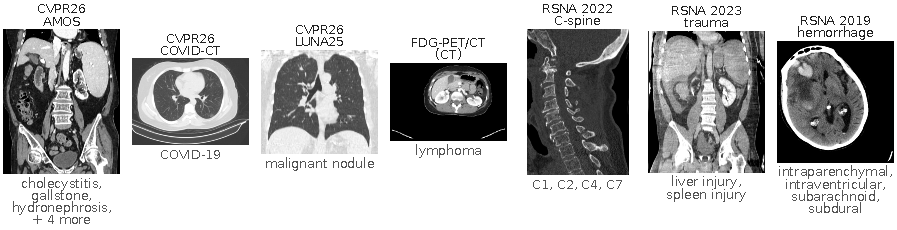
\includegraphics[width=\textwidth,height=0.74\textheight,keepaspectratio]{figures/fig_examples_cls.pdf}
\caption{One held-out case per classification source: the case with the most positive labels, listed below it. Views are fixed per source and pass through the body's center of mass: coronal for AMOS, LUNA25 and RSNA 2023, sagittal for the cervical spine, and axial for COVID-CTset (thick slices), FDG-PET/CT (whole body) and head CT. Windows are soft tissue, lung (COVID-CTset, LUNA25), bone (cervical spine) and brain (hemorrhage).}
\label{fig:examples}
\end{figure}

\begin{figure}[H]
\centering
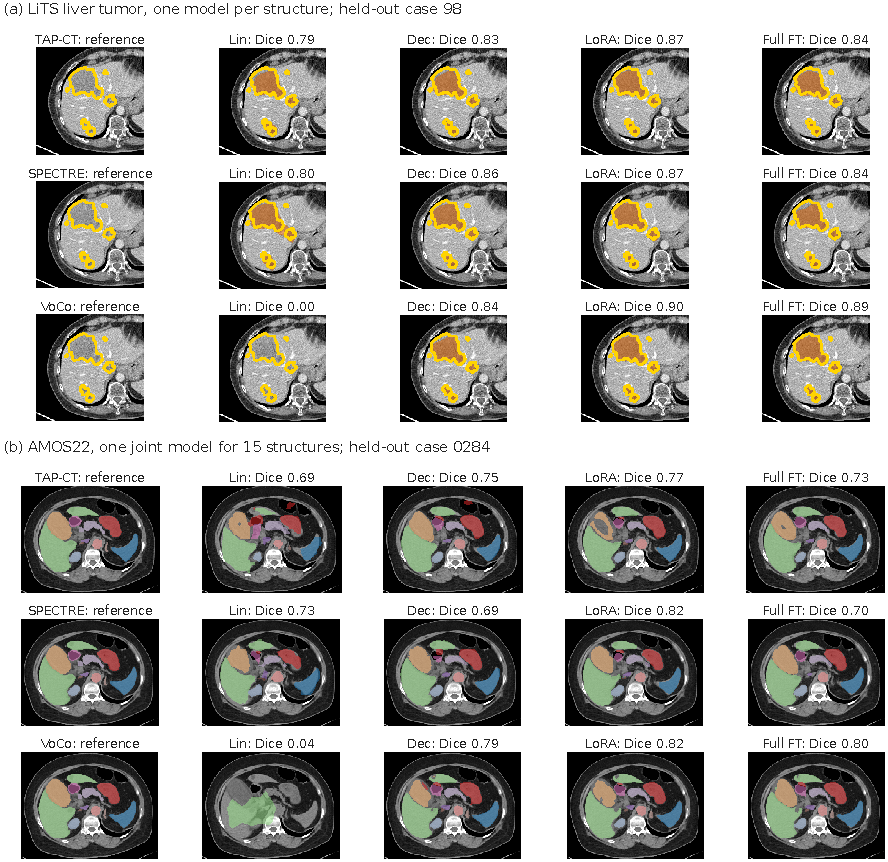
\includegraphics[width=0.94\textwidth,height=0.74\textheight,keepaspectratio]{figures/fig_examples_seg.pdf}
\caption{Segmentation examples on held-out cases, each on the backbone's own grid at the soft-tissue window; panel titles give the case's Dice (mean over structures in b). (a) LiTS liver tumor with one model per structure; yellow is the reference outline, orange the prediction. (b) AMOS22 with one joint model for all 15 structures (colors are structures). On TAP-CT and SPECTRE the decoder improves on the linear probe, LoRA has the highest Dice in both panels, and full fine-tuning does not improve on LoRA. On VoCo the linear probe predicts no tumor in (a) and almost nothing in (b). Cases were chosen by a fixed rule on TAP-CT and SPECTRE among held-out cases with a valid Dice in every run: the case agrees with each backbone's mean held-out Dice on the best and the worst method (a) or on the full ranking (b), and among such cases its pairwise Dice differences are closest to the mean differences; \numSegExLitsMatchN{} of \numSegExLitsCasesN{} cases qualify for (a) and \numSegExAmosMatchN{} of \numSegExAmosCasesN{} for (b).}
\label{fig:examplesseg}
\end{figure}

\clearpage
\section{Success and failure cases}
\label{app:cases}

\begin{figure}[H]
\centering
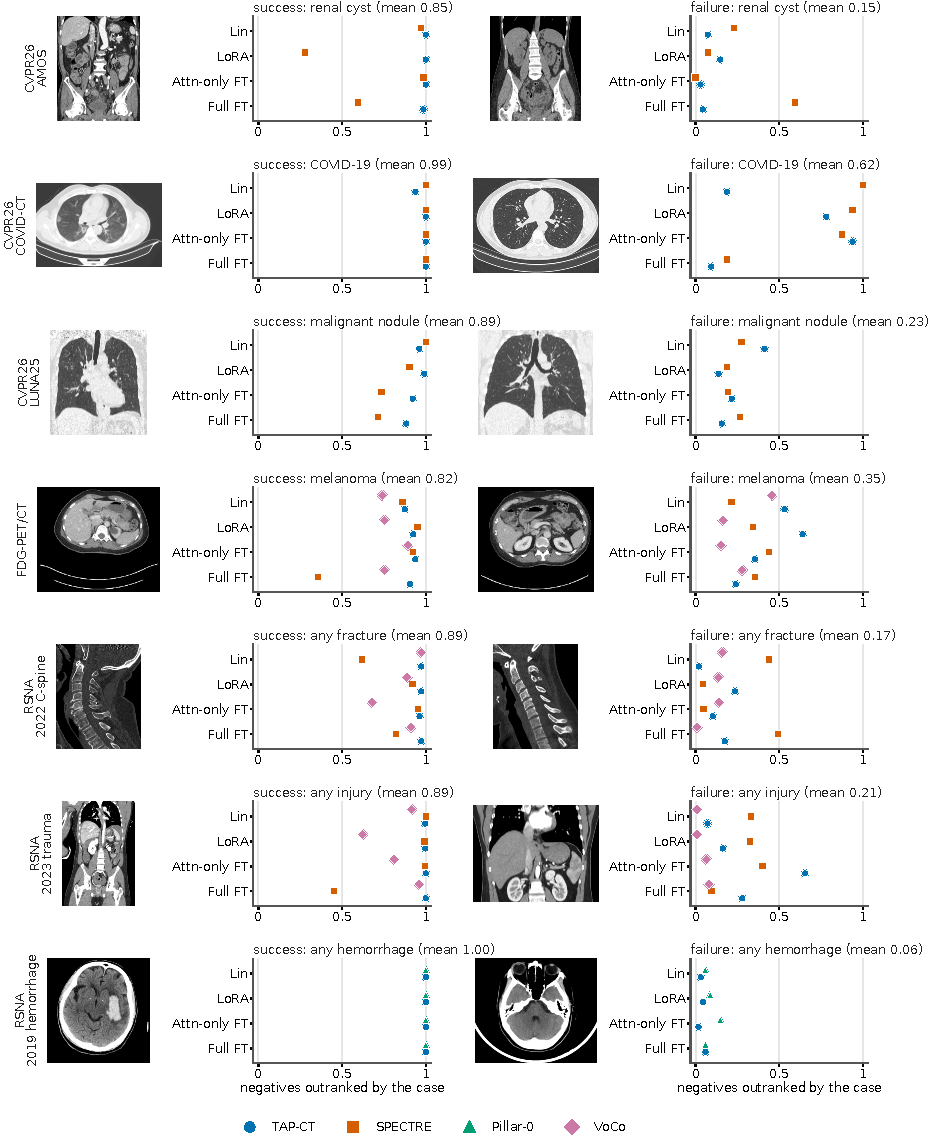
\includegraphics[width=\textwidth,height=0.74\textheight,keepaspectratio]{figures/fig_cases_cls.pdf}
\caption{Classification success (left) and failure (right) cases, one positive held-out case per source. Markers give the share of held-out negatives the case outranks for each method and backbone (1: ranked above every negative; dotted line: 0.5); the title gives the label and the case's mean over methods and backbones. Rows are the three CVPR26 sources, FDG-PET/CT, the RSNA 2022 cervical spine, RSNA 2023 trauma and RSNA 2019 hemorrhage.}
\label{fig:casescls}
\end{figure}

\begin{figure}[H]
\centering
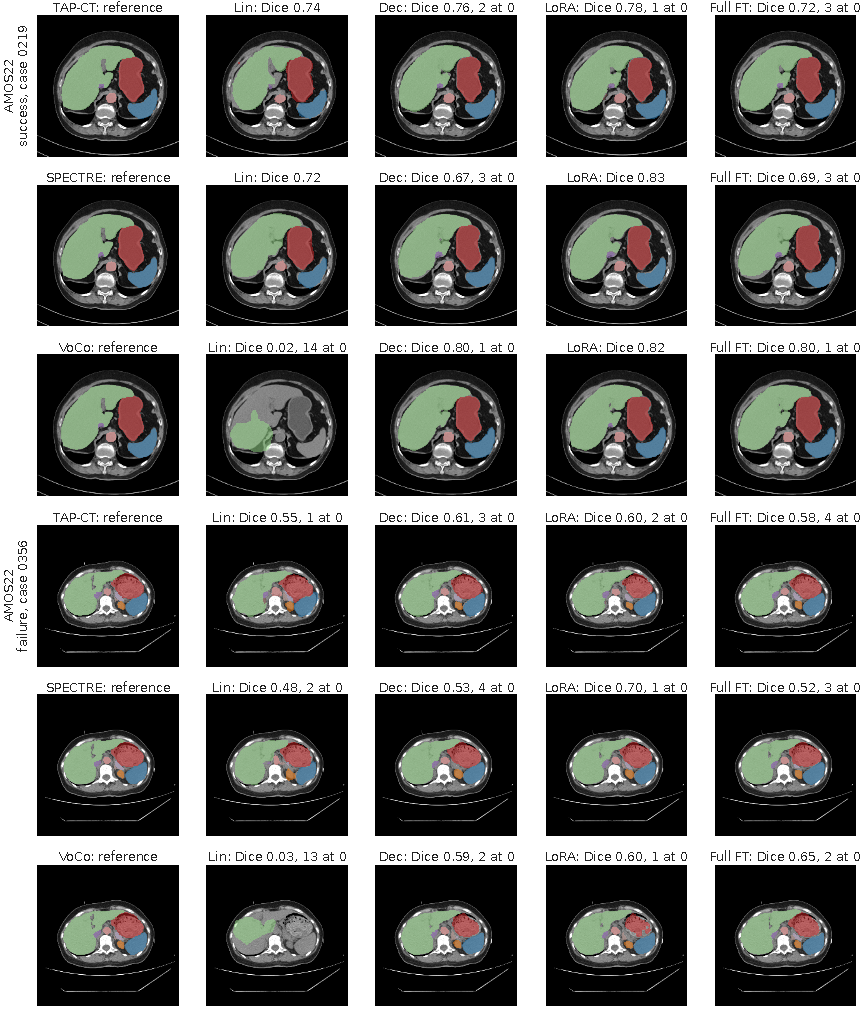
\includegraphics[width=0.9\textwidth,height=0.66\textheight,keepaspectratio]{figures/fig_cases_seg_amos22.pdf}
\caption{Segmentation success and failure cases on AMOS22 (15 structures), joint model. Rows: the success case (top three) and the failure case (bottom three), each on TAP-CT, SPECTRE and VoCo; columns: the reference and the predictions of Lin, Dec, LoRA and Full FT on the axial slice with the most reference foreground, soft-tissue window, colors per structure. Panel titles give the method's Dice for the whole case, averaged over its structures, and how many of them score 0. On TAP-CT and SPECTRE these are the adrenal glands for most adapted methods and, for some, the esophagus or the gallbladder. On VoCo the decoder and full fine-tuning score 0 on the prostate or uterus in both cases and on the right adrenal gland in the failure case, LoRA only on the right adrenal gland in the failure case, and the linear probe segments only the liver in both cases.}
\label{fig:casesseg_amos22}
\end{figure}

\begin{figure}[H]
\centering
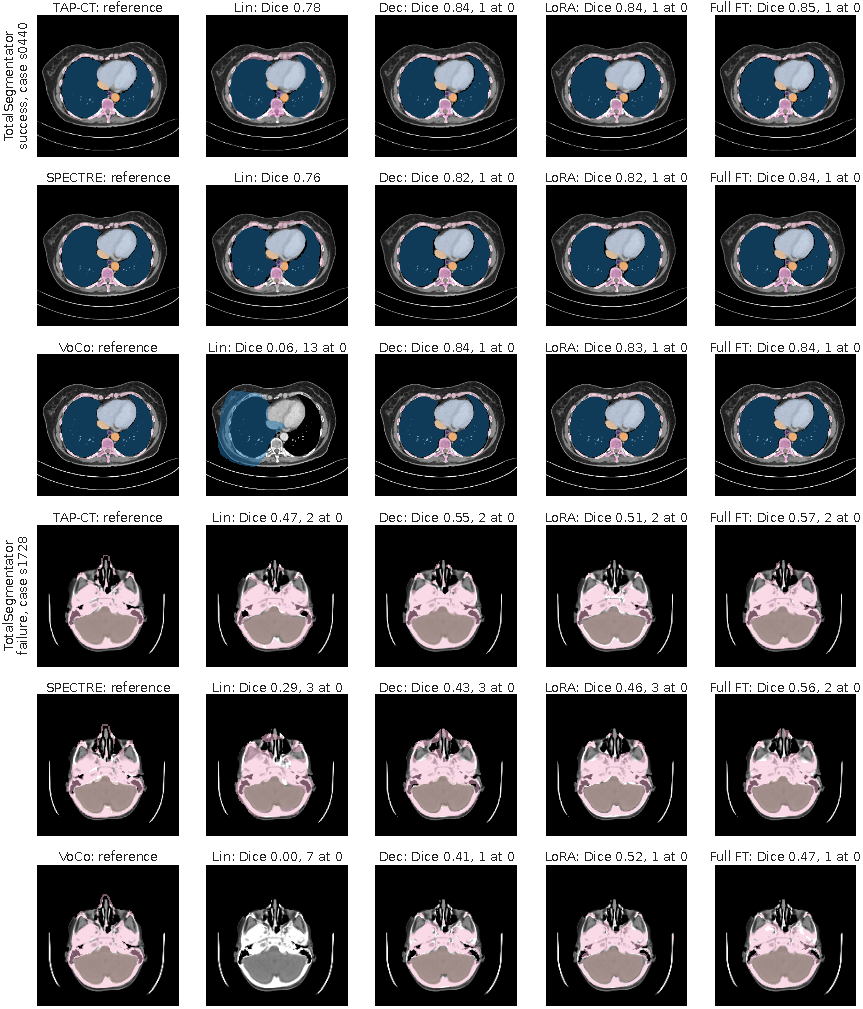
\includegraphics[width=0.9\textwidth,height=0.74\textheight,keepaspectratio]{figures/fig_cases_seg_totalseg.pdf}
\caption{As Figure~\ref{fig:casesseg_amos22}, for TotalSegmentator (15 merged structures). Every adapted joint model scores 0 on the merged glands in both cases; in the failure case some TAP-CT and SPECTRE models also score 0 on the arteries, the liver, the lungs and airway or the gastrointestinal tract. The VoCo linear probe scores 0 on 13 structures in the success case and on all 7 structures present in the failure case.}
\label{fig:casesseg_totalseg}
\end{figure}

\begin{figure}[H]
\centering
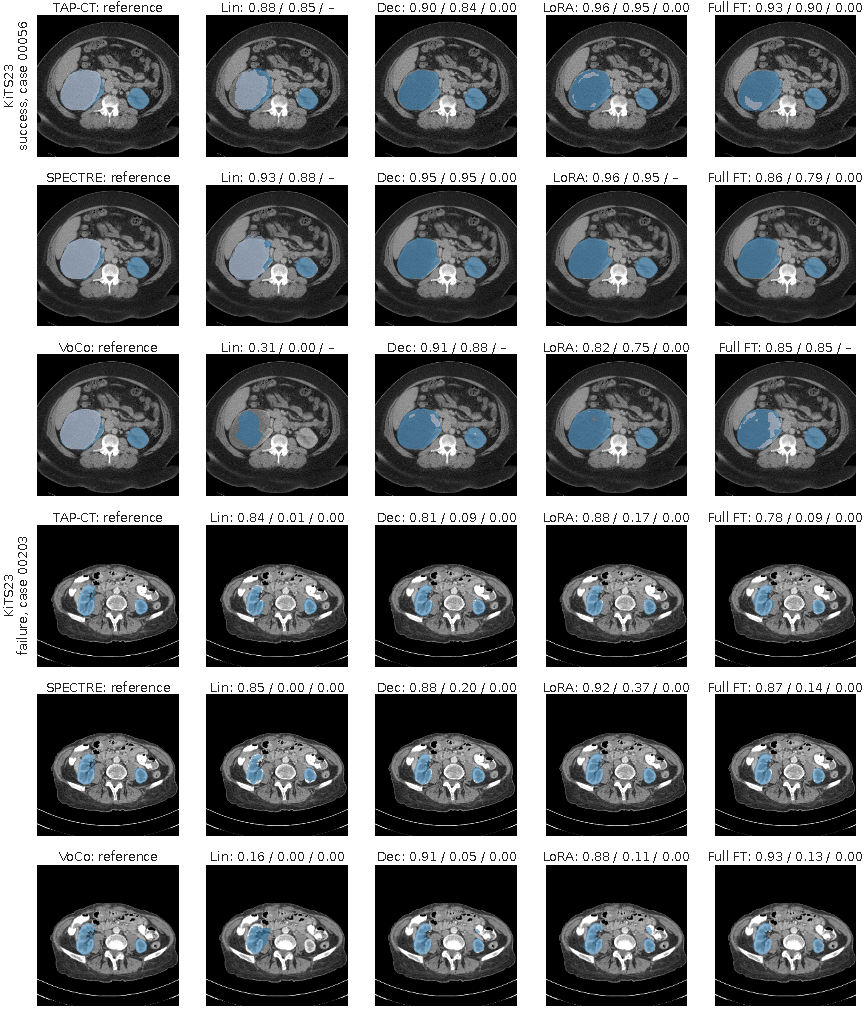
\includegraphics[width=0.9\textwidth,height=0.74\textheight,keepaspectratio]{figures/fig_cases_seg_kits23.pdf}
\caption{As Figure~\ref{fig:casesseg_amos22}, for KiTS23; panel titles give the Dice of each structure (kidney / tumor / cyst; \textendash: absent from both reference and prediction).}
\label{fig:casesseg_kits23}
\end{figure}

\begin{figure}[H]
\centering
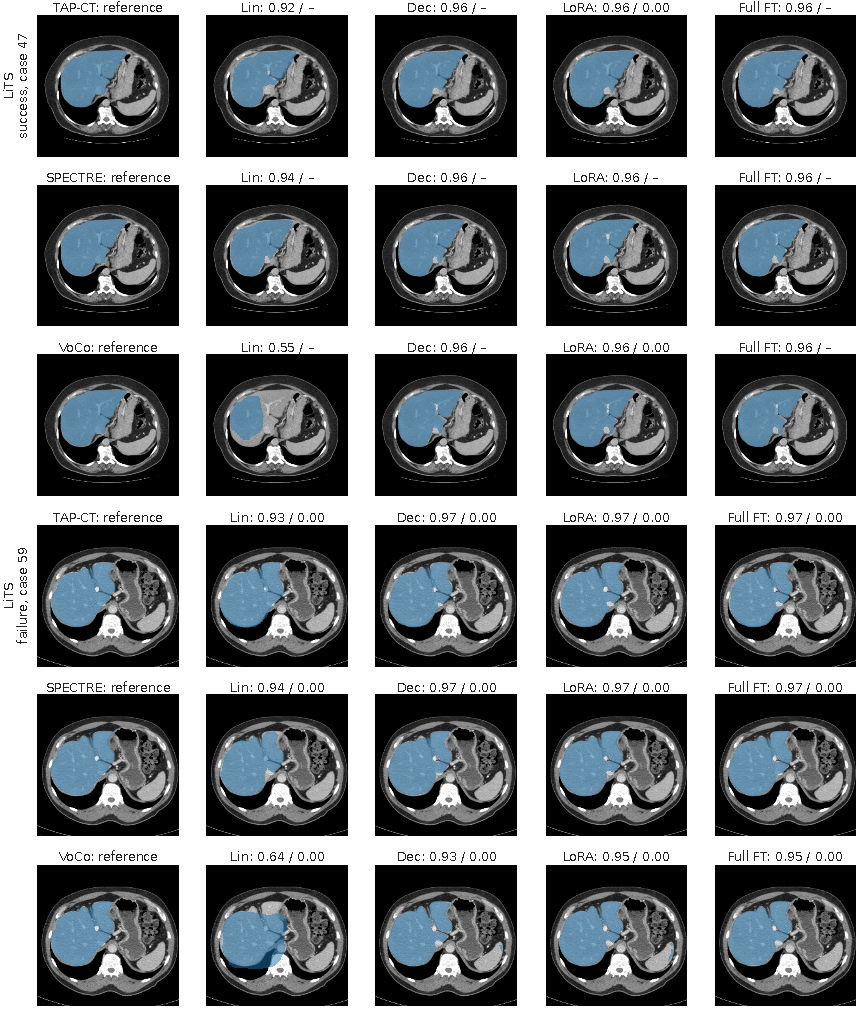
\includegraphics[width=0.9\textwidth,height=0.74\textheight,keepaspectratio]{figures/fig_cases_seg_lits.pdf}
\caption{As Figure~\ref{fig:casesseg_amos22}, for LiTS, except that panel titles give the Dice of each structure (liver / tumor; \textendash: absent from both reference and prediction). Neither case has a tumor in the reference, so a method's tumor Dice is undefined when it predicts no tumor and 0 when it predicts any: in the success case only LoRA on TAP-CT and on VoCo predict a tumor somewhere in the volume, and in the failure case every method does, while all segment the liver well. The failure is therefore a false-positive tumor, which the per-structure Dice counts as 0, and not a missed one; the overlay shows the structure with the highest logit at each voxel, which hides the predicted tumor under the liver in all but one run.}
\label{fig:casesseg_lits}
\end{figure}

\begin{figure}[H]
\centering
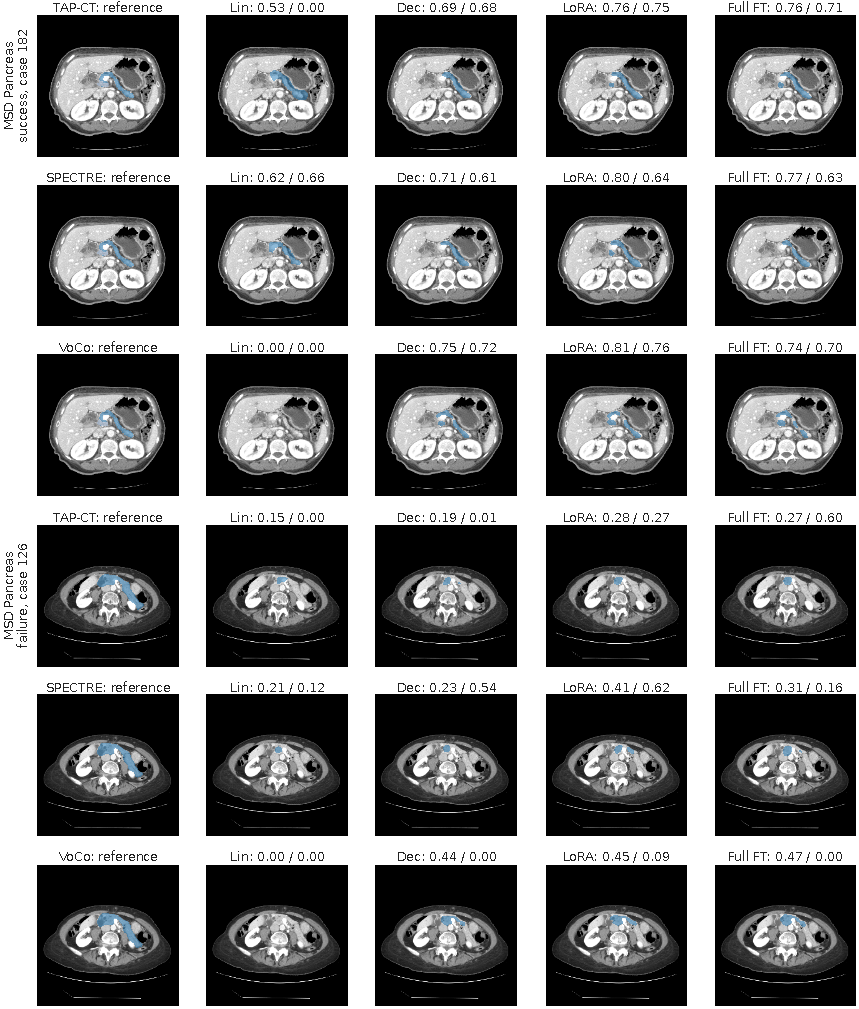
\includegraphics[width=0.9\textwidth,height=0.74\textheight,keepaspectratio]{figures/fig_cases_seg_msd_pancreas.pdf}
\caption{As Figure~\ref{fig:casesseg_amos22}, for MSD Pancreas; panel titles give the Dice of each structure (pancreas / tumor; \textendash: absent from both reference and prediction).}
\label{fig:casesseg_msd_pancreas}
\end{figure}
